\subsection{Diagrammi di classi}
I diagrammi di classi rappresentano il sistema della rubrica con le funzionalità di gestione dei contatti, dei tag, importazione/esportazione di dati, configurazioni e salvataggio dei dati in locale o su DB.
\begin{itemize}[noitemsep, topsep=5pt]
	\item \textbf{Contact}: Modella un contatto con attributi come nome, cognome, numeri di telefono, e-mail, immagine del profilo, e tag associati. Ha metodi per gestire i contatti, aggiungere e rimuovere numeri e e-mail, e per gestire i tag associati.
	\item \textbf{Tag}: Modella un'etichetta associata ai contatti, con attributi come id, descrizione, e un indice statico. Include metodi per ottenere e impostare descrizioni e id, e per confrontare gli oggetti.
	\item \textbf{AddressBook}: Contiene contatti e tag. È una classe singleton, quindi ha un'istanza unica, e gestisce il salvataggio dei dati tramite un database o la serializzazione. Ha metodi per aggiungere, rimuovere e ottenere contatti e tag, e per caricare e salvare i dati.
	\item \textbf{MainController}: Gestisce l'interfaccia utente principale, con metodi per inizializzare i componenti dell'interfaccia, aggiungere, modificare, rimuovere contatti, per visualizzare pop-up per l'importazione/esportazione e la gestione dei tag.
	\item \textbf{ImportPopupController}, \textbf{ExportPopupController}, \textbf{ManageTagsPopupController}, \textbf{ConfigPopupController}, \textbf{ImagePopupController}: Gestiscono i pop-up per importare/esportare contatti, gestire i tag, gestire la configurazione (link del DB) e gestire le immagini di profilo.
	\item \textbf{ConfirmPopupController}: Gestisce anch'essa un pop-up di conferma di un'eventuale operazione di eliminazione di un contatto o di un tag richiesta dall'utente.
	\item \textbf{Database}: Gestisce l'interazione con un database MongoDB per l'archiviazione di contatti e tag. Ha metodi per inserire, aggiornare, rimuovere, recuperare contatti e tag dal database.
	\item \textbf{Converter}: Classe di utilità finalizzata a determinate conversioni per Import ed Export.
\end{itemize}

\subsubsection{Livello di dettaglio basso}
\definecolor{plantucolor0000}{RGB}{241,241,241}
\definecolor{plantucolor0001}{RGB}{24,24,24}
\definecolor{plantucolor0002}{RGB}{173,209,178}
\definecolor{plantucolor0003}{RGB}{0,0,0}
\definecolor{plantucolor0004}{RGB}{200,41,48}
\definecolor{plantucolor0005}{RGB}{132,190,132}
\definecolor{plantucolor0006}{RGB}{3,128,72}
\definecolor{plantucolor0007}{RGB}{242,77,92}
\definecolor{plantucolor0008}{RGB}{180,167,229}

\begin{adjustbox}{width=.95\paperwidth, center}
	\resizebox{\textwidth}{!}{
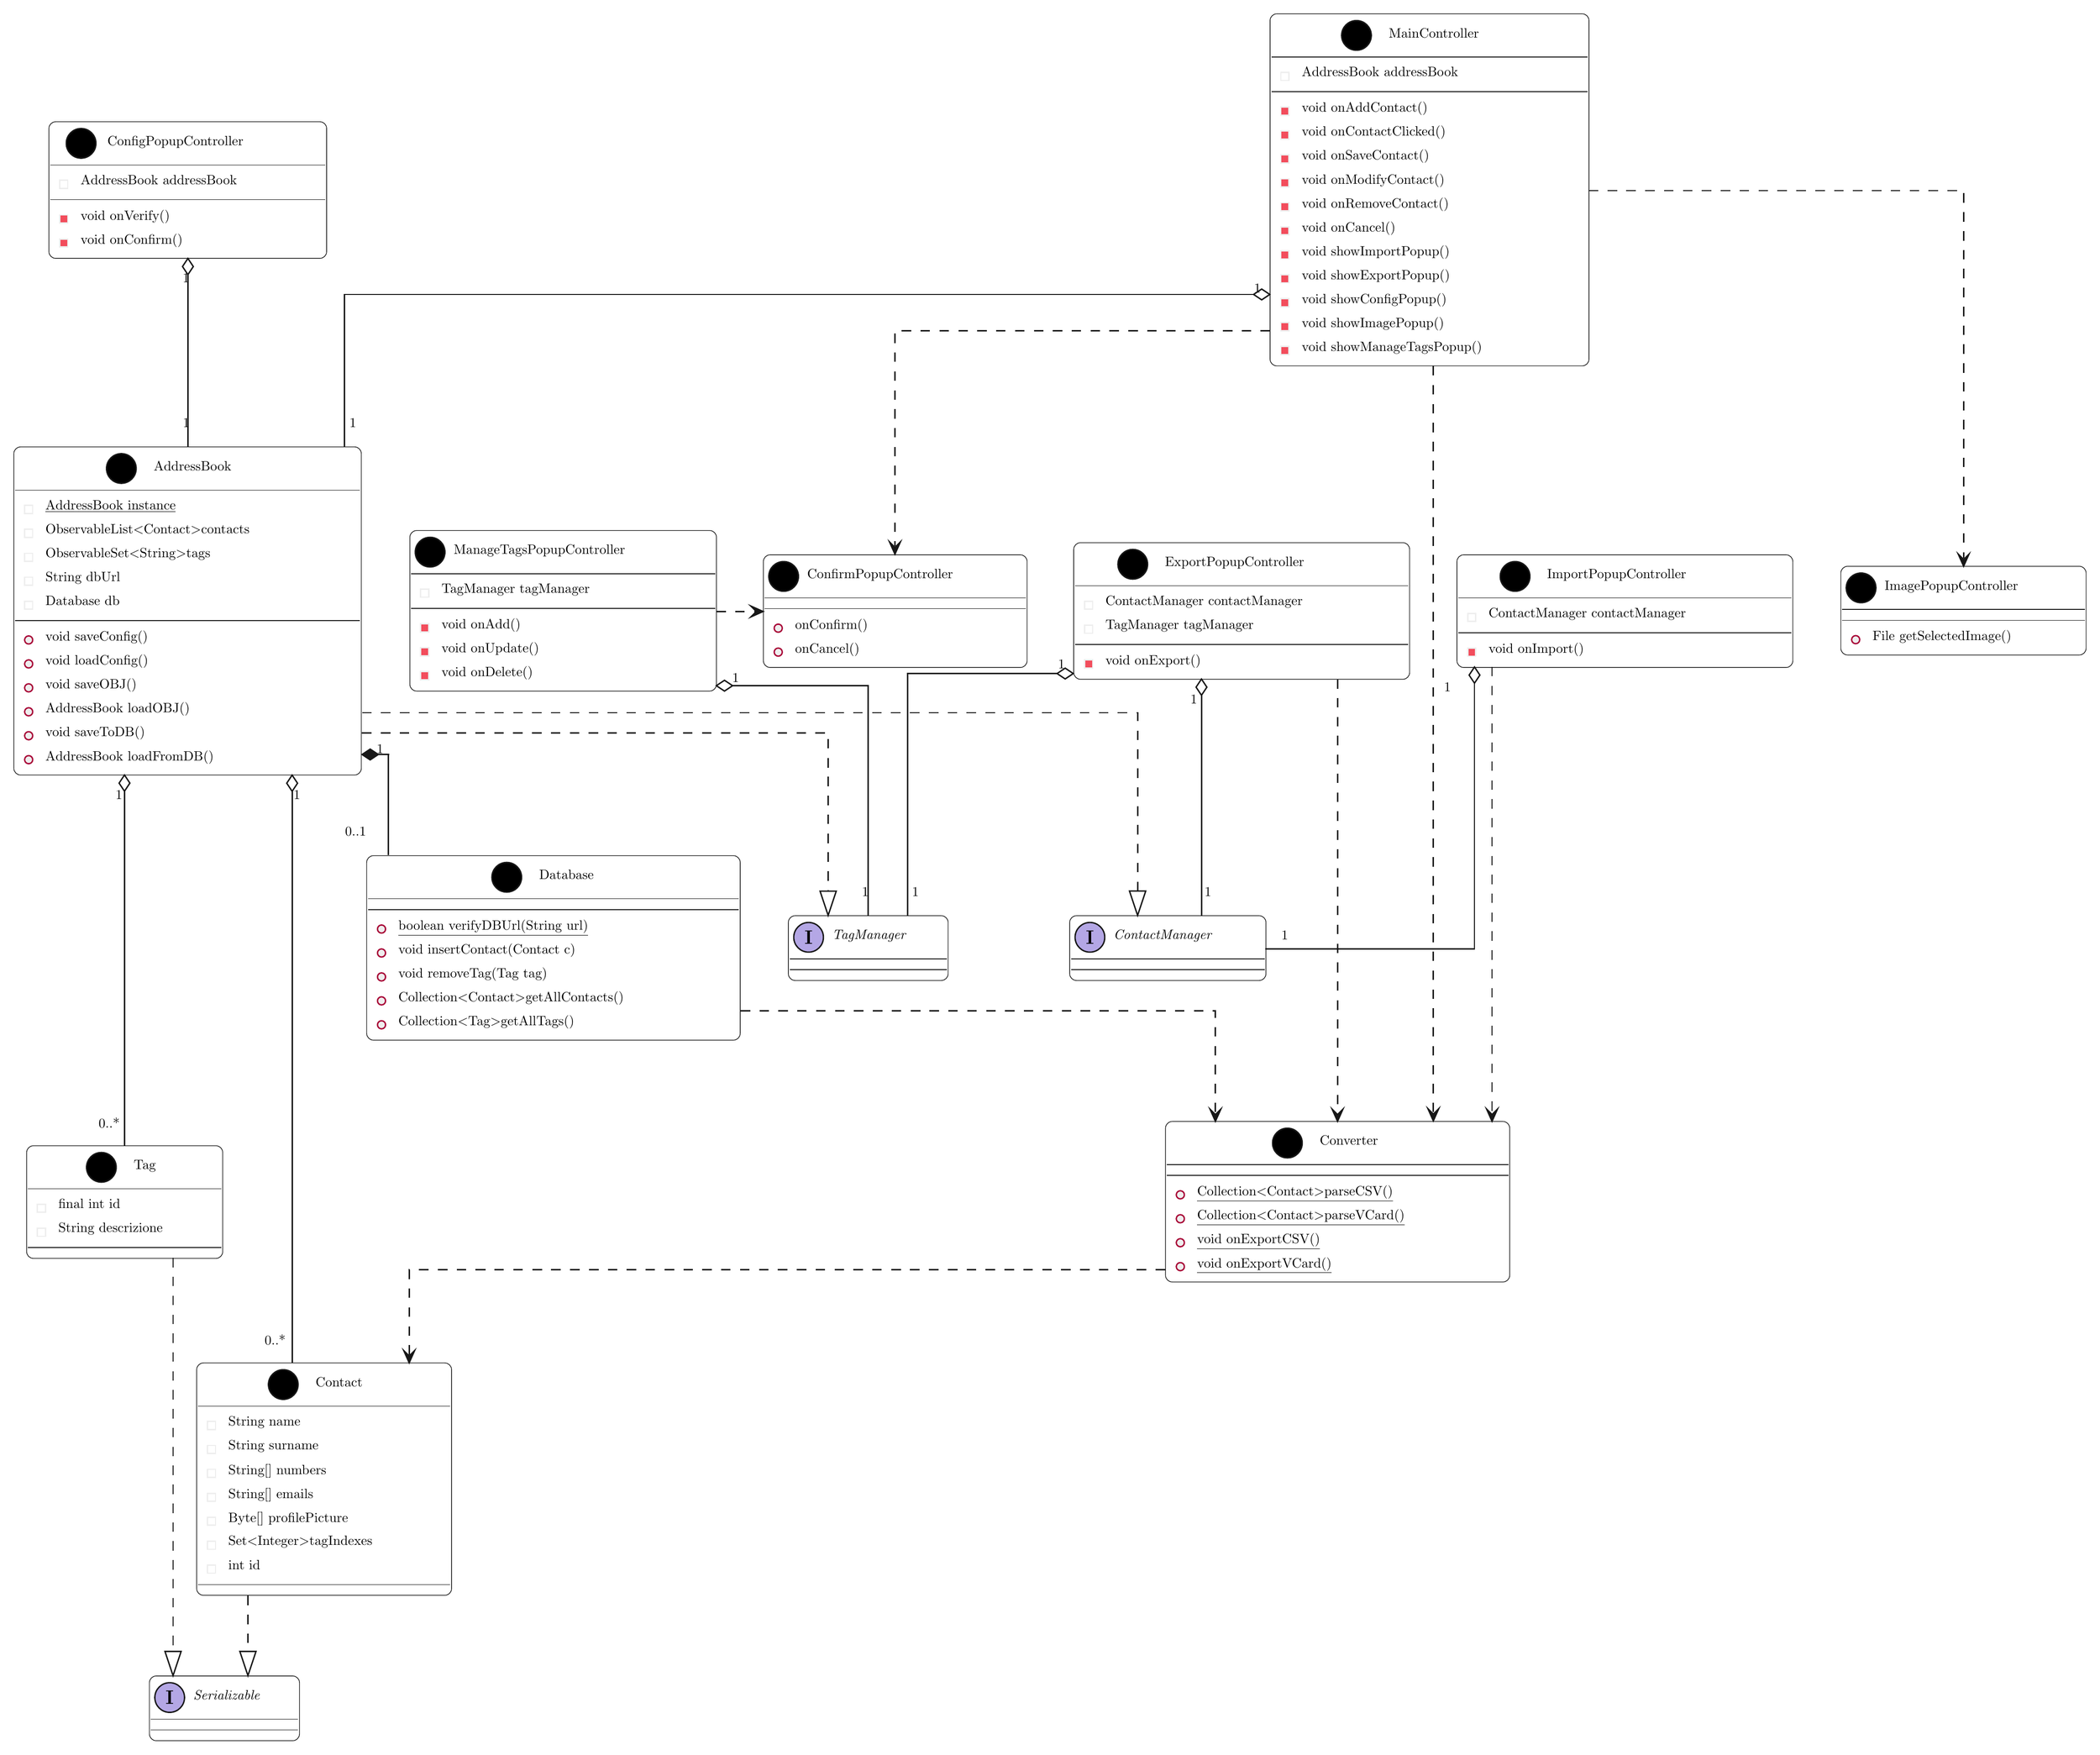
\begin{tikzpicture}[yscale=-1
,pstyle0/.style={color=plantucolor0001,fill=plantucolor0000,line width=0.5pt}
,pstyle1/.style={color=plantucolor0001,fill=plantucolor0002,line width=1.0pt}
,pstyle2/.style={color=plantucolor0001,line width=0.5pt}
,pstyle3/.style={color=plantucolor0004,line width=1.0pt}
,pstyle4/.style={color=plantucolor0006,fill=plantucolor0005,line width=1.0pt}
,pstyle5/.style={color=plantucolor0004,fill=plantucolor0007,line width=1.0pt}
,pstyle6/.style={color=plantucolor0001,fill=plantucolor0008,line width=1.0pt}
,pstyle7/.style={color=plantucolor0001,line width=1.0pt,dash pattern=on 7.0pt off 7.0pt}
,pstyle8/.style={color=plantucolor0001,line width=1.0pt}
,pstyle9/.style={color=plantucolor0001,fill=plantucolor0001,line width=1.0pt}
]
\draw[pstyle0] (142.5pt,1012pt) arc (180:270:5pt) -- (147.5pt,1007pt) -- (326.4151pt,1007pt) arc (270:360:5pt) -- (331.4151pt,1012pt) -- (331.4151pt,1174.2227pt) arc (0:90:5pt) -- (326.4151pt,1179.2227pt) -- (147.5pt,1179.2227pt) arc (90:180:5pt) -- (142.5pt,1174.2227pt) -- cycle;
\draw[pstyle1] (206.6712pt,1023pt) ellipse (11pt and 11pt);
\node at (206.6712pt,1023pt)[]{\textbf{\Large C}};
\node at (227.1712pt,1014.127pt)[below right,color=black]{Contact};
\draw[pstyle2] (143.5pt,1039pt) -- (330.4151pt,1039pt);
\draw[pstyle3] (150.5pt,1050.373pt) rectangle (156.5pt,1056.373pt);
\node at (162.5pt,1043pt)[below right,color=black]{String name};
\draw[pstyle3] (150.5pt,1068.1191pt) rectangle (156.5pt,1074.1191pt);
\node at (162.5pt,1060.7461pt)[below right,color=black]{String surname};
\draw[pstyle3] (150.5pt,1085.8652pt) rectangle (156.5pt,1091.8652pt);
\node at (162.5pt,1078.4922pt)[below right,color=black]{String[] numbers};
\draw[pstyle3] (150.5pt,1103.6113pt) rectangle (156.5pt,1109.6113pt);
\node at (162.5pt,1096.2383pt)[below right,color=black]{String[] emails};
\draw[pstyle3] (150.5pt,1121.3574pt) rectangle (156.5pt,1127.3574pt);
\node at (162.5pt,1113.9844pt)[below right,color=black]{Byte[] profilePicture};
\draw[pstyle3] (150.5pt,1139.1035pt) rectangle (156.5pt,1145.1035pt);
\node at (162.5pt,1131.7305pt)[below right,color=black]{Set\textless Integer\textgreater  tagIndexes};
\draw[pstyle3] (150.5pt,1156.8496pt) rectangle (156.5pt,1162.8496pt);
\node at (162.5pt,1149.4766pt)[below right,color=black]{int id};
\draw[pstyle2] (143.5pt,1171.2227pt) -- (330.4151pt,1171.2227pt);
\draw[pstyle0] (7pt,333pt) arc (180:270:5pt) -- (12pt,328pt) -- (259.5265pt,328pt) arc (270:360:5pt) -- (264.5265pt,333pt) -- (264.5265pt,566.207pt) arc (0:90:5pt) -- (259.5265pt,571.207pt) -- (12pt,571.207pt) arc (90:180:5pt) -- (7pt,566.207pt) -- cycle;
\draw[pstyle1] (86.6733pt,344pt) ellipse (11pt and 11pt);
\node at (86.6733pt,344pt)[]{\textbf{\Large C}};
\node at (107.1733pt,335.127pt)[below right,color=black]{AddressBook};
\draw[pstyle2] (8pt,360pt) -- (263.5265pt,360pt);
\draw[pstyle3] (15pt,371.373pt) rectangle (21pt,377.373pt);
\node at (27pt,364pt)[below right,color=black]{\underline{AddressBook instance}};
\draw[pstyle3] (15pt,389.1191pt) rectangle (21pt,395.1191pt);
\node at (27pt,381.7461pt)[below right,color=black]{ObservableList\textless Contact\textgreater  contacts};
\draw[pstyle3] (15pt,406.8652pt) rectangle (21pt,412.8652pt);
\node at (27pt,399.4922pt)[below right,color=black]{ObservableSet\textless String\textgreater  tags};
\draw[pstyle3] (15pt,424.6113pt) rectangle (21pt,430.6113pt);
\node at (27pt,417.2383pt)[below right,color=black]{String dbUrl};
\draw[pstyle3] (15pt,442.3574pt) rectangle (21pt,448.3574pt);
\node at (27pt,434.9844pt)[below right,color=black]{Database db};
\draw[pstyle2] (8pt,456.7305pt) -- (263.5265pt,456.7305pt);
\draw[pstyle4] (18pt,471.1035pt) ellipse (3pt and 3pt);
\node at (27pt,460.7305pt)[below right,color=black]{void saveConfig()};
\draw[pstyle4] (18pt,488.8496pt) ellipse (3pt and 3pt);
\node at (27pt,478.4766pt)[below right,color=black]{void loadConfig()};
\draw[pstyle4] (18pt,506.5957pt) ellipse (3pt and 3pt);
\node at (27pt,496.2227pt)[below right,color=black]{void saveOBJ()};
\draw[pstyle4] (18pt,524.3418pt) ellipse (3pt and 3pt);
\node at (27pt,513.9688pt)[below right,color=black]{AddressBook loadOBJ()};
\draw[pstyle4] (18pt,542.0879pt) ellipse (3pt and 3pt);
\node at (27pt,531.7148pt)[below right,color=black]{void saveToDB()};
\draw[pstyle4] (18pt,559.834pt) ellipse (3pt and 3pt);
\node at (27pt,549.4609pt)[below right,color=black]{AddressBook loadFromDB()};
\draw[pstyle0] (938pt,12pt) arc (180:270:5pt) -- (943pt,7pt) -- (1169.3435pt,7pt) arc (270:360:5pt) -- (1174.3435pt,12pt) -- (1174.3435pt,262.9531pt) arc (0:90:5pt) -- (1169.3435pt,267.9531pt) -- (943pt,267.9531pt) arc (90:180:5pt) -- (938pt,262.9531pt) -- cycle;
\draw[pstyle1] (1002.0218pt,23pt) ellipse (11pt and 11pt);
\node at (1002.0218pt,23pt)[]{\textbf{\Large C}};
\node at (1022.5218pt,14.127pt)[below right,color=black]{MainController};
\draw[pstyle2] (939pt,39pt) -- (1173.3435pt,39pt);
\draw[pstyle3] (946pt,50.373pt) rectangle (952pt,56.373pt);
\node at (958pt,43pt)[below right,color=black]{AddressBook addressBook};
\draw[pstyle2] (939pt,64.7461pt) -- (1173.3435pt,64.7461pt);
\draw[pstyle5] (946pt,76.1191pt) rectangle (952pt,82.1191pt);
\node at (958pt,68.7461pt)[below right,color=black]{void onAddContact()};
\draw[pstyle5] (946pt,93.8652pt) rectangle (952pt,99.8652pt);
\node at (958pt,86.4922pt)[below right,color=black]{void onContactClicked()};
\draw[pstyle5] (946pt,111.6113pt) rectangle (952pt,117.6113pt);
\node at (958pt,104.2383pt)[below right,color=black]{void onSaveContact()};
\draw[pstyle5] (946pt,129.3574pt) rectangle (952pt,135.3574pt);
\node at (958pt,121.9844pt)[below right,color=black]{void onModifyContact()};
\draw[pstyle5] (946pt,147.1035pt) rectangle (952pt,153.1035pt);
\node at (958pt,139.7305pt)[below right,color=black]{void onRemoveContact()};
\draw[pstyle5] (946pt,164.8496pt) rectangle (952pt,170.8496pt);
\node at (958pt,157.4766pt)[below right,color=black]{void onCancel()};
\draw[pstyle5] (946pt,182.5957pt) rectangle (952pt,188.5957pt);
\node at (958pt,175.2227pt)[below right,color=black]{void showImportPopup()};
\draw[pstyle5] (946pt,200.3418pt) rectangle (952pt,206.3418pt);
\node at (958pt,192.9688pt)[below right,color=black]{void showExportPopup()};
\draw[pstyle5] (946pt,218.0879pt) rectangle (952pt,224.0879pt);
\node at (958pt,210.7148pt)[below right,color=black]{void showConfigPopup()};
\draw[pstyle5] (946pt,235.834pt) rectangle (952pt,241.834pt);
\node at (958pt,228.4609pt)[below right,color=black]{void showImagePopup()};
\draw[pstyle5] (946pt,253.5801pt) rectangle (952pt,259.5801pt);
\node at (958pt,246.207pt)[below right,color=black]{void showManageTagsPopup()};
\draw[pstyle0] (860.5pt,833pt) arc (180:270:5pt) -- (865.5pt,828pt) -- (1110.598pt,828pt) arc (270:360:5pt) -- (1115.598pt,833pt) -- (1115.598pt,941.9844pt) arc (0:90:5pt) -- (1110.598pt,946.9844pt) -- (865.5pt,946.9844pt) arc (90:180:5pt) -- (860.5pt,941.9844pt) -- cycle;
\draw[pstyle1] (950.8418pt,844pt) ellipse (11pt and 11pt);
\node at (950.8418pt,844pt)[]{\textbf{\Large C}};
\node at (971.3418pt,835.127pt)[below right,color=black]{Converter};
\draw[pstyle2] (861.5pt,860pt) -- (1114.598pt,860pt);
\draw[pstyle2] (861.5pt,868pt) -- (1114.598pt,868pt);
\draw[pstyle4] (871.5pt,882.373pt) ellipse (3pt and 3pt);
\node at (880.5pt,872pt)[below right,color=black]{\underline{Collection\textless Contact\textgreater  parseCSV()}};
\draw[pstyle4] (871.5pt,900.1191pt) ellipse (3pt and 3pt);
\node at (880.5pt,889.7461pt)[below right,color=black]{\underline{Collection\textless Contact\textgreater  parseVCard()}};
\draw[pstyle4] (871.5pt,917.8652pt) ellipse (3pt and 3pt);
\node at (880.5pt,907.4922pt)[below right,color=black]{\underline{void onExportCSV()}};
\draw[pstyle4] (871.5pt,935.6113pt) ellipse (3pt and 3pt);
\node at (880.5pt,925.2383pt)[below right,color=black]{\underline{void onExportVCard()}};
\draw[pstyle0] (1076.5pt,413pt) arc (180:270:5pt) -- (1081.5pt,408pt) -- (1320.4191pt,408pt) arc (270:360:5pt) -- (1325.4191pt,413pt) -- (1325.4191pt,486.4922pt) arc (0:90:5pt) -- (1320.4191pt,491.4922pt) -- (1081.5pt,491.4922pt) arc (90:180:5pt) -- (1076.5pt,486.4922pt) -- cycle;
\draw[pstyle1] (1119.5828pt,424pt) ellipse (11pt and 11pt);
\node at (1119.5828pt,424pt)[]{\textbf{\Large C}};
\node at (1139.8234pt,415.127pt)[below right,color=black]{ImportPopupController};
\draw[pstyle2] (1077.5pt,440pt) -- (1324.4191pt,440pt);
\draw[pstyle3] (1084.5pt,451.373pt) rectangle (1090.5pt,457.373pt);
\node at (1096.5pt,444pt)[below right,color=black]{ContactManager contactManager};
\draw[pstyle2] (1077.5pt,465.7461pt) -- (1324.4191pt,465.7461pt);
\draw[pstyle5] (1084.5pt,477.1191pt) rectangle (1090.5pt,483.1191pt);
\node at (1096.5pt,469.7461pt)[below right,color=black]{void onImport()};
\draw[pstyle0] (792.5pt,404pt) arc (180:270:5pt) -- (797.5pt,399pt) -- (1036.4191pt,399pt) arc (270:360:5pt) -- (1041.4191pt,404pt) -- (1041.4191pt,495.2383pt) arc (0:90:5pt) -- (1036.4191pt,500.2383pt) -- (797.5pt,500.2383pt) arc (90:180:5pt) -- (792.5pt,495.2383pt) -- cycle;
\draw[pstyle1] (836.2428pt,415pt) ellipse (11pt and 11pt);
\node at (836.2428pt,415pt)[]{\textbf{\Large C}};
\node at (856.6301pt,406.127pt)[below right,color=black]{ExportPopupController};
\draw[pstyle2] (793.5pt,431pt) -- (1040.4191pt,431pt);
\draw[pstyle3] (800.5pt,442.373pt) rectangle (806.5pt,448.373pt);
\node at (812.5pt,435pt)[below right,color=black]{ContactManager contactManager};
\draw[pstyle3] (800.5pt,460.1191pt) rectangle (806.5pt,466.1191pt);
\node at (812.5pt,452.7461pt)[below right,color=black]{TagManager tagManager};
\draw[pstyle2] (793.5pt,474.4922pt) -- (1040.4191pt,474.4922pt);
\draw[pstyle5] (800.5pt,485.8652pt) rectangle (806.5pt,491.8652pt);
\node at (812.5pt,478.4922pt)[below right,color=black]{void onExport()};
\draw[pstyle0] (300.5pt,395pt) arc (180:270:5pt) -- (305.5pt,390pt) -- (522.7146pt,390pt) arc (270:360:5pt) -- (527.7146pt,395pt) -- (527.7146pt,503.9844pt) arc (0:90:5pt) -- (522.7146pt,508.9844pt) -- (305.5pt,508.9844pt) arc (90:180:5pt) -- (300.5pt,503.9844pt) -- cycle;
\draw[pstyle1] (315.5pt,406pt) ellipse (11pt and 11pt);
\node at (315.5pt,406pt)[]{\textbf{\Large C}};
\node at (329.5pt,397.127pt)[below right,color=black]{ManageTagsPopupController};
\draw[pstyle2] (301.5pt,422pt) -- (526.7146pt,422pt);
\draw[pstyle3] (308.5pt,433.373pt) rectangle (314.5pt,439.373pt);
\node at (320.5pt,426pt)[below right,color=black]{TagManager tagManager};
\draw[pstyle2] (301.5pt,447.7461pt) -- (526.7146pt,447.7461pt);
\draw[pstyle5] (308.5pt,459.1191pt) rectangle (314.5pt,465.1191pt);
\node at (320.5pt,451.7461pt)[below right,color=black]{void onAdd()};
\draw[pstyle5] (308.5pt,476.8652pt) rectangle (314.5pt,482.8652pt);
\node at (320.5pt,469.4922pt)[below right,color=black]{void onUpdate()};
\draw[pstyle5] (308.5pt,494.6113pt) rectangle (314.5pt,500.6113pt);
\node at (320.5pt,487.2383pt)[below right,color=black]{void onDelete()};
\draw[pstyle0] (1361pt,421.5pt) arc (180:270:5pt) -- (1366pt,416.5pt) -- (1537.7543pt,416.5pt) arc (270:360:5pt) -- (1542.7543pt,421.5pt) -- (1542.7543pt,477.2461pt) arc (0:90:5pt) -- (1537.7543pt,482.2461pt) -- (1366pt,482.2461pt) arc (90:180:5pt) -- (1361pt,477.2461pt) -- cycle;
\draw[pstyle1] (1376pt,432.5pt) ellipse (11pt and 11pt);
\node at (1376pt,432.5pt)[]{\textbf{\Large C}};
\node at (1390pt,423.627pt)[below right,color=black]{ImagePopupController};
\draw[pstyle2] (1362pt,448.5pt) -- (1541.7543pt,448.5pt);
\draw[pstyle2] (1362pt,456.5pt) -- (1541.7543pt,456.5pt);
\draw[pstyle4] (1372pt,470.873pt) ellipse (3pt and 3pt);
\node at (1381pt,460.5pt)[below right,color=black]{File getSelectedImage()};
\draw[pstyle0] (562.5pt,413pt) arc (180:270:5pt) -- (567.5pt,408pt) -- (752.9331pt,408pt) arc (270:360:5pt) -- (757.9331pt,413pt) -- (757.9331pt,486.4922pt) arc (0:90:5pt) -- (752.9331pt,491.4922pt) -- (567.5pt,491.4922pt) arc (90:180:5pt) -- (562.5pt,486.4922pt) -- cycle;
\draw[pstyle1] (577.5pt,424pt) ellipse (11pt and 11pt);
\node at (577.5pt,424pt)[]{\textbf{\Large C}};
\node at (591.5pt,415.127pt)[below right,color=black]{ConfirmPopupController};
\draw[pstyle2] (563.5pt,440pt) -- (756.9331pt,440pt);
\draw[pstyle2] (563.5pt,448pt) -- (756.9331pt,448pt);
\draw[pstyle4] (573.5pt,462.373pt) ellipse (3pt and 3pt);
\node at (582.5pt,452pt)[below right,color=black]{onConfirm()};
\draw[pstyle4] (573.5pt,480.1191pt) ellipse (3pt and 3pt);
\node at (582.5pt,469.7461pt)[below right,color=black]{onCancel()};
\draw[pstyle0] (33pt,92pt) arc (180:270:5pt) -- (38pt,87pt) -- (233.8225pt,87pt) arc (270:360:5pt) -- (238.8225pt,92pt) -- (238.8225pt,183.2383pt) arc (0:90:5pt) -- (233.8225pt,188.2383pt) -- (38pt,188.2383pt) arc (90:180:5pt) -- (33pt,183.2383pt) -- cycle;
\draw[pstyle1] (56.8509pt,103pt) ellipse (11pt and 11pt);
\node at (56.8509pt,103pt)[]{\textbf{\Large C}};
\node at (72.8178pt,94.127pt)[below right,color=black]{ConfigPopupController};
\draw[pstyle2] (34pt,119pt) -- (237.8225pt,119pt);
\draw[pstyle3] (41pt,130.373pt) rectangle (47pt,136.373pt);
\node at (53pt,123pt)[below right,color=black]{AddressBook addressBook};
\draw[pstyle2] (34pt,144.7461pt) -- (237.8225pt,144.7461pt);
\draw[pstyle5] (41pt,156.1191pt) rectangle (47pt,162.1191pt);
\node at (53pt,148.7461pt)[below right,color=black]{void onVerify()};
\draw[pstyle5] (41pt,173.8652pt) rectangle (47pt,179.8652pt);
\node at (53pt,166.4922pt)[below right,color=black]{void onConfirm()};
\draw[pstyle0] (16.5pt,851pt) arc (180:270:5pt) -- (21.5pt,846pt) -- (156.799pt,846pt) arc (270:360:5pt) -- (161.799pt,851pt) -- (161.799pt,924.4922pt) arc (0:90:5pt) -- (156.799pt,929.4922pt) -- (21.5pt,929.4922pt) arc (90:180:5pt) -- (16.5pt,924.4922pt) -- cycle;
\draw[pstyle1] (71.8813pt,862pt) ellipse (11pt and 11pt);
\node at (71.8813pt,862pt)[]{\textbf{\Large C}};
\node at (92.3813pt,853.127pt)[below right,color=black]{Tag};
\draw[pstyle2] (17.5pt,878pt) -- (160.799pt,878pt);
\draw[pstyle3] (24.5pt,889.373pt) rectangle (30.5pt,895.373pt);
\node at (36.5pt,882pt)[below right,color=black]{final int id};
\draw[pstyle3] (24.5pt,907.1191pt) rectangle (30.5pt,913.1191pt);
\node at (36.5pt,899.7461pt)[below right,color=black]{String descrizione};
\draw[pstyle2] (17.5pt,921.4922pt) -- (160.799pt,921.4922pt);
\draw[pstyle0] (268.5pt,636pt) arc (180:270:5pt) -- (273.5pt,631pt) -- (540.3151pt,631pt) arc (270:360:5pt) -- (545.3151pt,636pt) -- (545.3151pt,762.7305pt) arc (0:90:5pt) -- (540.3151pt,767.7305pt) -- (273.5pt,767.7305pt) arc (90:180:5pt) -- (268.5pt,762.7305pt) -- cycle;
\draw[pstyle1] (372.2928pt,647pt) ellipse (11pt and 11pt);
\node at (372.2928pt,647pt)[]{\textbf{\Large C}};
\node at (392.7928pt,638.127pt)[below right,color=black]{Database};
\draw[pstyle2] (269.5pt,663pt) -- (544.3151pt,663pt);
\draw[pstyle2] (269.5pt,671pt) -- (544.3151pt,671pt);
\draw[pstyle4] (279.5pt,685.373pt) ellipse (3pt and 3pt);
\node at (288.5pt,675pt)[below right,color=black]{\underline{boolean verifyDBUrl(String url)}};
\draw[pstyle4] (279.5pt,703.1191pt) ellipse (3pt and 3pt);
\node at (288.5pt,692.7461pt)[below right,color=black]{void insertContact(Contact c)};
\draw[pstyle4] (279.5pt,720.8652pt) ellipse (3pt and 3pt);
\node at (288.5pt,710.4922pt)[below right,color=black]{void removeTag(Tag tag)};
\draw[pstyle4] (279.5pt,738.6113pt) ellipse (3pt and 3pt);
\node at (288.5pt,728.2383pt)[below right,color=black]{Collection\textless Contact\textgreater  getAllContacts()};
\draw[pstyle4] (279.5pt,756.3574pt) ellipse (3pt and 3pt);
\node at (288.5pt,745.9844pt)[below right,color=black]{Collection\textless Tag\textgreater  getAllTags()};
\draw[pstyle0] (107.5pt,1244pt) arc (180:270:5pt) -- (112.5pt,1239pt) -- (213.7pt,1239pt) arc (270:360:5pt) -- (218.7pt,1244pt) -- (218.7pt,1282pt) arc (0:90:5pt) -- (213.7pt,1287pt) -- (112.5pt,1287pt) arc (90:180:5pt) -- (107.5pt,1282pt) -- cycle;
\draw[pstyle6] (122.5pt,1255pt) ellipse (11pt and 11pt);
\node at (122.5pt,1255pt)[]{\textbf{\Large I}};
\node at (136.5pt,1246.127pt)[below right,color=black]{\textit{Serializable}};
\draw[pstyle2] (108.5pt,1271pt) -- (217.7pt,1271pt);
\draw[pstyle2] (108.5pt,1279pt) -- (217.7pt,1279pt);
\draw[pstyle0] (581pt,680.5pt) arc (180:270:5pt) -- (586pt,675.5pt) -- (694.3945pt,675.5pt) arc (270:360:5pt) -- (699.3945pt,680.5pt) -- (699.3945pt,718.5pt) arc (0:90:5pt) -- (694.3945pt,723.5pt) -- (586pt,723.5pt) arc (90:180:5pt) -- (581pt,718.5pt) -- cycle;
\draw[pstyle6] (596pt,691.5pt) ellipse (11pt and 11pt);
\node at (596pt,691.5pt)[]{\textbf{\Large I}};
\node at (610pt,682.627pt)[below right,color=black]{\textit{TagManager}};
\draw[pstyle2] (582pt,707.5pt) -- (698.3945pt,707.5pt);
\draw[pstyle2] (582pt,715.5pt) -- (698.3945pt,715.5pt);
\draw[pstyle0] (789.5pt,680.5pt) arc (180:270:5pt) -- (794.5pt,675.5pt) -- (929.9526pt,675.5pt) arc (270:360:5pt) -- (934.9526pt,680.5pt) -- (934.9526pt,718.5pt) arc (0:90:5pt) -- (929.9526pt,723.5pt) -- (794.5pt,723.5pt) arc (90:180:5pt) -- (789.5pt,718.5pt) -- cycle;
\draw[pstyle6] (804.5pt,691.5pt) ellipse (11pt and 11pt);
\node at (804.5pt,691.5pt)[]{\textbf{\Large I}};
\node at (818.5pt,682.627pt)[below right,color=black]{\textit{ContactManager}};
\draw[pstyle2] (790.5pt,707.5pt) -- (933.9526pt,707.5pt);
\draw[pstyle2] (790.5pt,715.5pt) -- (933.9526pt,715.5pt);
\draw[pstyle7] (180.5pt,1179.49pt) ..controls (180.5pt,1201.31pt) and (180.5pt,1205pt) .. (180.5pt,1220.8pt);
\draw[pstyle8] (180.5pt,1238.8pt) -- (186.5pt,1220.8pt) -- (174.5pt,1220.8pt) -- (180.5pt,1238.8pt) -- cycle;
\draw[pstyle7] (125pt,929.12pt) ..controls (125pt,1007.79pt) and (125pt,1158.05pt) .. (125pt,1220.77pt);
\draw[pstyle8] (125pt,1238.77pt) -- (131pt,1220.77pt) -- (119pt,1220.77pt) -- (125pt,1238.77pt) -- cycle;
\draw[pstyle8] (213.25pt,583.29pt) ..controls (213.25pt,710.46pt) and (213.25pt,894.66pt) .. (213.25pt,1006.7pt);
\draw[pstyle8] (213.25pt,571.29pt) -- (209.25pt,577.29pt) -- (213.25pt,583.29pt) -- (217.25pt,577.29pt) -- (213.25pt,571.29pt) -- cycle;
\node at (210.7647pt,579.2073pt)[below right,color=black]{1};
\node at (189.3514pt,982.6071pt)[below right,color=black]{0..*};
\draw[pstyle8] (277.09pt,556pt) ..controls (288.88pt,556pt) and (284.5pt,556pt) .. (284.5pt,556pt) ..controls (284.5pt,556pt) and (284.5pt,593.86pt) .. (284.5pt,630.69pt);
\draw[pstyle9] (265.09pt,556pt) -- (271.09pt,560pt) -- (277.09pt,556pt) -- (271.09pt,552pt) -- (265.09pt,556pt) -- cycle;
\node at (272.3594pt,545.3941pt)[below right,color=black]{1};
\node at (248.996pt,606.3298pt)[below right,color=black]{0..1};
\draw[pstyle8] (89pt,583.22pt) ..controls (89pt,674.98pt) and (89pt,783.35pt) .. (89pt,845.82pt);
\draw[pstyle8] (89pt,571.22pt) -- (85pt,577.22pt) -- (89pt,583.22pt) -- (93pt,577.22pt) -- (89pt,571.22pt) -- cycle;
\node at (78.9432pt,579.1331pt)[below right,color=black]{1};
\node at (66.3155pt,821.5906pt)[below right,color=black]{0..*};
\draw[pstyle7] (265.03pt,540pt) ..controls (405.54pt,540pt) and (610.5pt,540pt) .. (610.5pt,540pt) ..controls (610.5pt,540pt) and (610.5pt,612.66pt) .. (610.5pt,657.28pt);
\draw[pstyle8] (610.5pt,675.28pt) -- (616.5pt,657.28pt) -- (604.5pt,657.28pt) -- (610.5pt,675.28pt) -- cycle;
\draw[pstyle7] (265.09pt,525pt) ..controls (468.28pt,525pt) and (839.83pt,525pt) .. (839.83pt,525pt) ..controls (839.83pt,525pt) and (839.83pt,609.29pt) .. (839.83pt,657.24pt);
\draw[pstyle8] (839.83pt,675.24pt) -- (845.83pt,657.24pt) -- (833.83pt,657.24pt) -- (839.83pt,675.24pt) -- cycle;
\draw[pstyle8] (925.8pt,215pt) ..controls (702.32pt,215pt) and (252pt,215pt) .. (252pt,215pt) ..controls (252pt,215pt) and (252pt,270.69pt) .. (252pt,327.79pt);
\draw[pstyle8] (937.8pt,215pt) -- (931.8pt,211pt) -- (925.8pt,215pt) -- (931.8pt,219pt) -- (937.8pt,215pt) -- cycle;
\node at (922.6185pt,203.6872pt)[below right,color=black]{1};
\node at (252.2286pt,303.4891pt)[below right,color=black]{1};
\draw[pstyle7] (1174.01pt,138pt) ..controls (1290.72pt,138pt) and (1452pt,138pt) .. (1452pt,138pt) ..controls (1452pt,138pt) and (1452pt,330.29pt) .. (1452pt,410.46pt);
\draw[pstyle9] (1452pt,416.46pt) -- (1456pt,407.46pt) -- (1452pt,411.46pt) -- (1448pt,407.46pt) -- (1452pt,416.46pt) -- cycle;
\draw[pstyle7] (937.99pt,242pt) ..controls (821.28pt,242pt) and (660pt,242pt) .. (660pt,242pt) ..controls (660pt,242pt) and (660pt,340.88pt) .. (660pt,401.51pt);
\draw[pstyle9] (660pt,407.51pt) -- (664pt,398.51pt) -- (660pt,402.51pt) -- (656pt,398.51pt) -- (660pt,407.51pt) -- cycle;
\draw[pstyle7] (1059pt,268.14pt) ..controls (1059pt,432.24pt) and (1059pt,700.91pt) .. (1059pt,821.57pt);
\draw[pstyle9] (1059pt,827.57pt) -- (1063pt,818.57pt) -- (1059pt,822.57pt) -- (1055pt,818.57pt) -- (1059pt,827.57pt) -- cycle;
\draw[pstyle7] (860.2pt,938pt) ..controls (661.24pt,938pt) and (300pt,938pt) .. (300pt,938pt) ..controls (300pt,938pt) and (300pt,965.21pt) .. (300pt,1000.89pt);
\draw[pstyle9] (300pt,1006.89pt) -- (304pt,997.89pt) -- (300pt,1001.89pt) -- (296pt,997.89pt) -- (300pt,1006.89pt) -- cycle;
\draw[pstyle8] (1089.5pt,503.15pt) ..controls (1089.5pt,574.38pt) and (1089.5pt,700pt) .. (1089.5pt,700pt) ..controls (1089.5pt,700pt) and (1001.19pt,700pt) .. (934.61pt,700pt);
\draw[pstyle8] (1089.5pt,491.15pt) -- (1085.5pt,497.15pt) -- (1089.5pt,503.15pt) -- (1093.5pt,497.15pt) -- (1089.5pt,491.15pt) -- cycle;
\node at (1063.4764pt,499.3721pt)[below right,color=black]{1};
\node at (942.9207pt,683.2059pt)[below right,color=black]{1};
\draw[pstyle7] (1102.5pt,491.1pt) ..controls (1102.5pt,569.15pt) and (1102.5pt,731.77pt) .. (1102.5pt,821.88pt);
\draw[pstyle9] (1102.5pt,827.88pt) -- (1106.5pt,818.88pt) -- (1102.5pt,822.88pt) -- (1098.5pt,818.88pt) -- (1102.5pt,827.88pt) -- cycle;
\draw[pstyle8] (887.17pt,512.09pt) ..controls (887.17pt,565.45pt) and (887.17pt,635.26pt) .. (887.17pt,675.48pt);
\draw[pstyle8] (887.17pt,500.09pt) -- (883.17pt,506.09pt) -- (887.17pt,512.09pt) -- (891.17pt,506.09pt) -- (887.17pt,500.09pt) -- cycle;
\node at (875.5027pt,508.3461pt)[below right,color=black]{1};
\node at (885.9599pt,650.9389pt)[below right,color=black]{1};
\draw[pstyle8] (780.16pt,496pt) ..controls (718.65pt,496pt) and (669.5pt,496pt) .. (669.5pt,496pt) ..controls (669.5pt,496pt) and (669.5pt,621.45pt) .. (669.5pt,675.36pt);
\draw[pstyle8] (792.16pt,496pt) -- (786.16pt,492pt) -- (780.16pt,496pt) -- (786.16pt,500pt) -- (792.16pt,496pt) -- cycle;
\node at (777.3478pt,482.3534pt)[below right,color=black]{1};
\node at (669.1376pt,651.1854pt)[below right,color=black]{1};
\draw[pstyle7] (988pt,500.17pt) ..controls (988pt,581.58pt) and (988pt,735.12pt) .. (988pt,821.88pt);
\draw[pstyle9] (988pt,827.88pt) -- (992pt,818.88pt) -- (988pt,822.88pt) -- (984pt,818.88pt) -- (988pt,827.88pt) -- cycle;
\draw[pstyle7] (527.64pt,450pt) ..controls (539.22pt,450pt) and (544.91pt,450pt) .. (556.3pt,450pt);
\draw[pstyle9] (562.3pt,450pt) -- (553.3pt,446pt) -- (557.3pt,450pt) -- (553.3pt,454pt) -- (562.3pt,450pt) -- cycle;
\draw[pstyle8] (539.66pt,505pt) ..controls (595.94pt,505pt) and (640pt,505pt) .. (640pt,505pt) ..controls (640pt,505pt) and (640pt,623.12pt) .. (640pt,675.26pt);
\draw[pstyle8] (527.66pt,505pt) -- (533.66pt,509pt) -- (539.66pt,505pt) -- (533.66pt,501pt) -- (527.66pt,505pt) -- cycle;
\node at (535.8973pt,492.3572pt)[below right,color=black]{1};
\node at (632.0782pt,651.0598pt)[below right,color=black]{1};
\draw[pstyle8] (136pt,200.32pt) ..controls (136pt,238.14pt) and (136pt,279.39pt) .. (136pt,327.95pt);
\draw[pstyle8] (136pt,188.32pt) -- (132pt,194.32pt) -- (136pt,200.32pt) -- (140pt,194.32pt) -- (136pt,188.32pt) -- cycle;
\node at (128.555pt,196.2401pt)[below right,color=black]{1};
\node at (128.7974pt,303.6594pt)[below right,color=black]{1};
\draw[pstyle7] (545.59pt,746pt) ..controls (690.64pt,746pt) and (897.5pt,746pt) .. (897.5pt,746pt) ..controls (897.5pt,746pt) and (897.5pt,783.23pt) .. (897.5pt,821.9pt);
\draw[pstyle9] (897.5pt,827.9pt) -- (901.5pt,818.9pt) -- (897.5pt,822.9pt) -- (893.5pt,818.9pt) -- (897.5pt,827.9pt) -- cycle;
\end{tikzpicture}
}
\end{adjustbox}
\begin{figure}[h]
	\caption{Diagramma classi essenziale}
	\label{fig:Diagramma classi essenziale}
\end{figure}
\newpage
\subsubsection{Livello di dettaglio alto}
\definecolor{plantucolor0000}{RGB}{241,241,241}
\definecolor{plantucolor0001}{RGB}{24,24,24}
\definecolor{plantucolor0002}{RGB}{173,209,178}
\definecolor{plantucolor0003}{RGB}{0,0,0}
\definecolor{plantucolor0004}{RGB}{200,41,48}
\definecolor{plantucolor0005}{RGB}{132,190,132}
\definecolor{plantucolor0006}{RGB}{3,128,72}
\definecolor{plantucolor0007}{RGB}{242,77,92}
\definecolor{plantucolor0008}{RGB}{180,167,229}

\begin{adjustbox}{width=.99\paperwidth, center}
	\resizebox{\textwidth}{!}{
		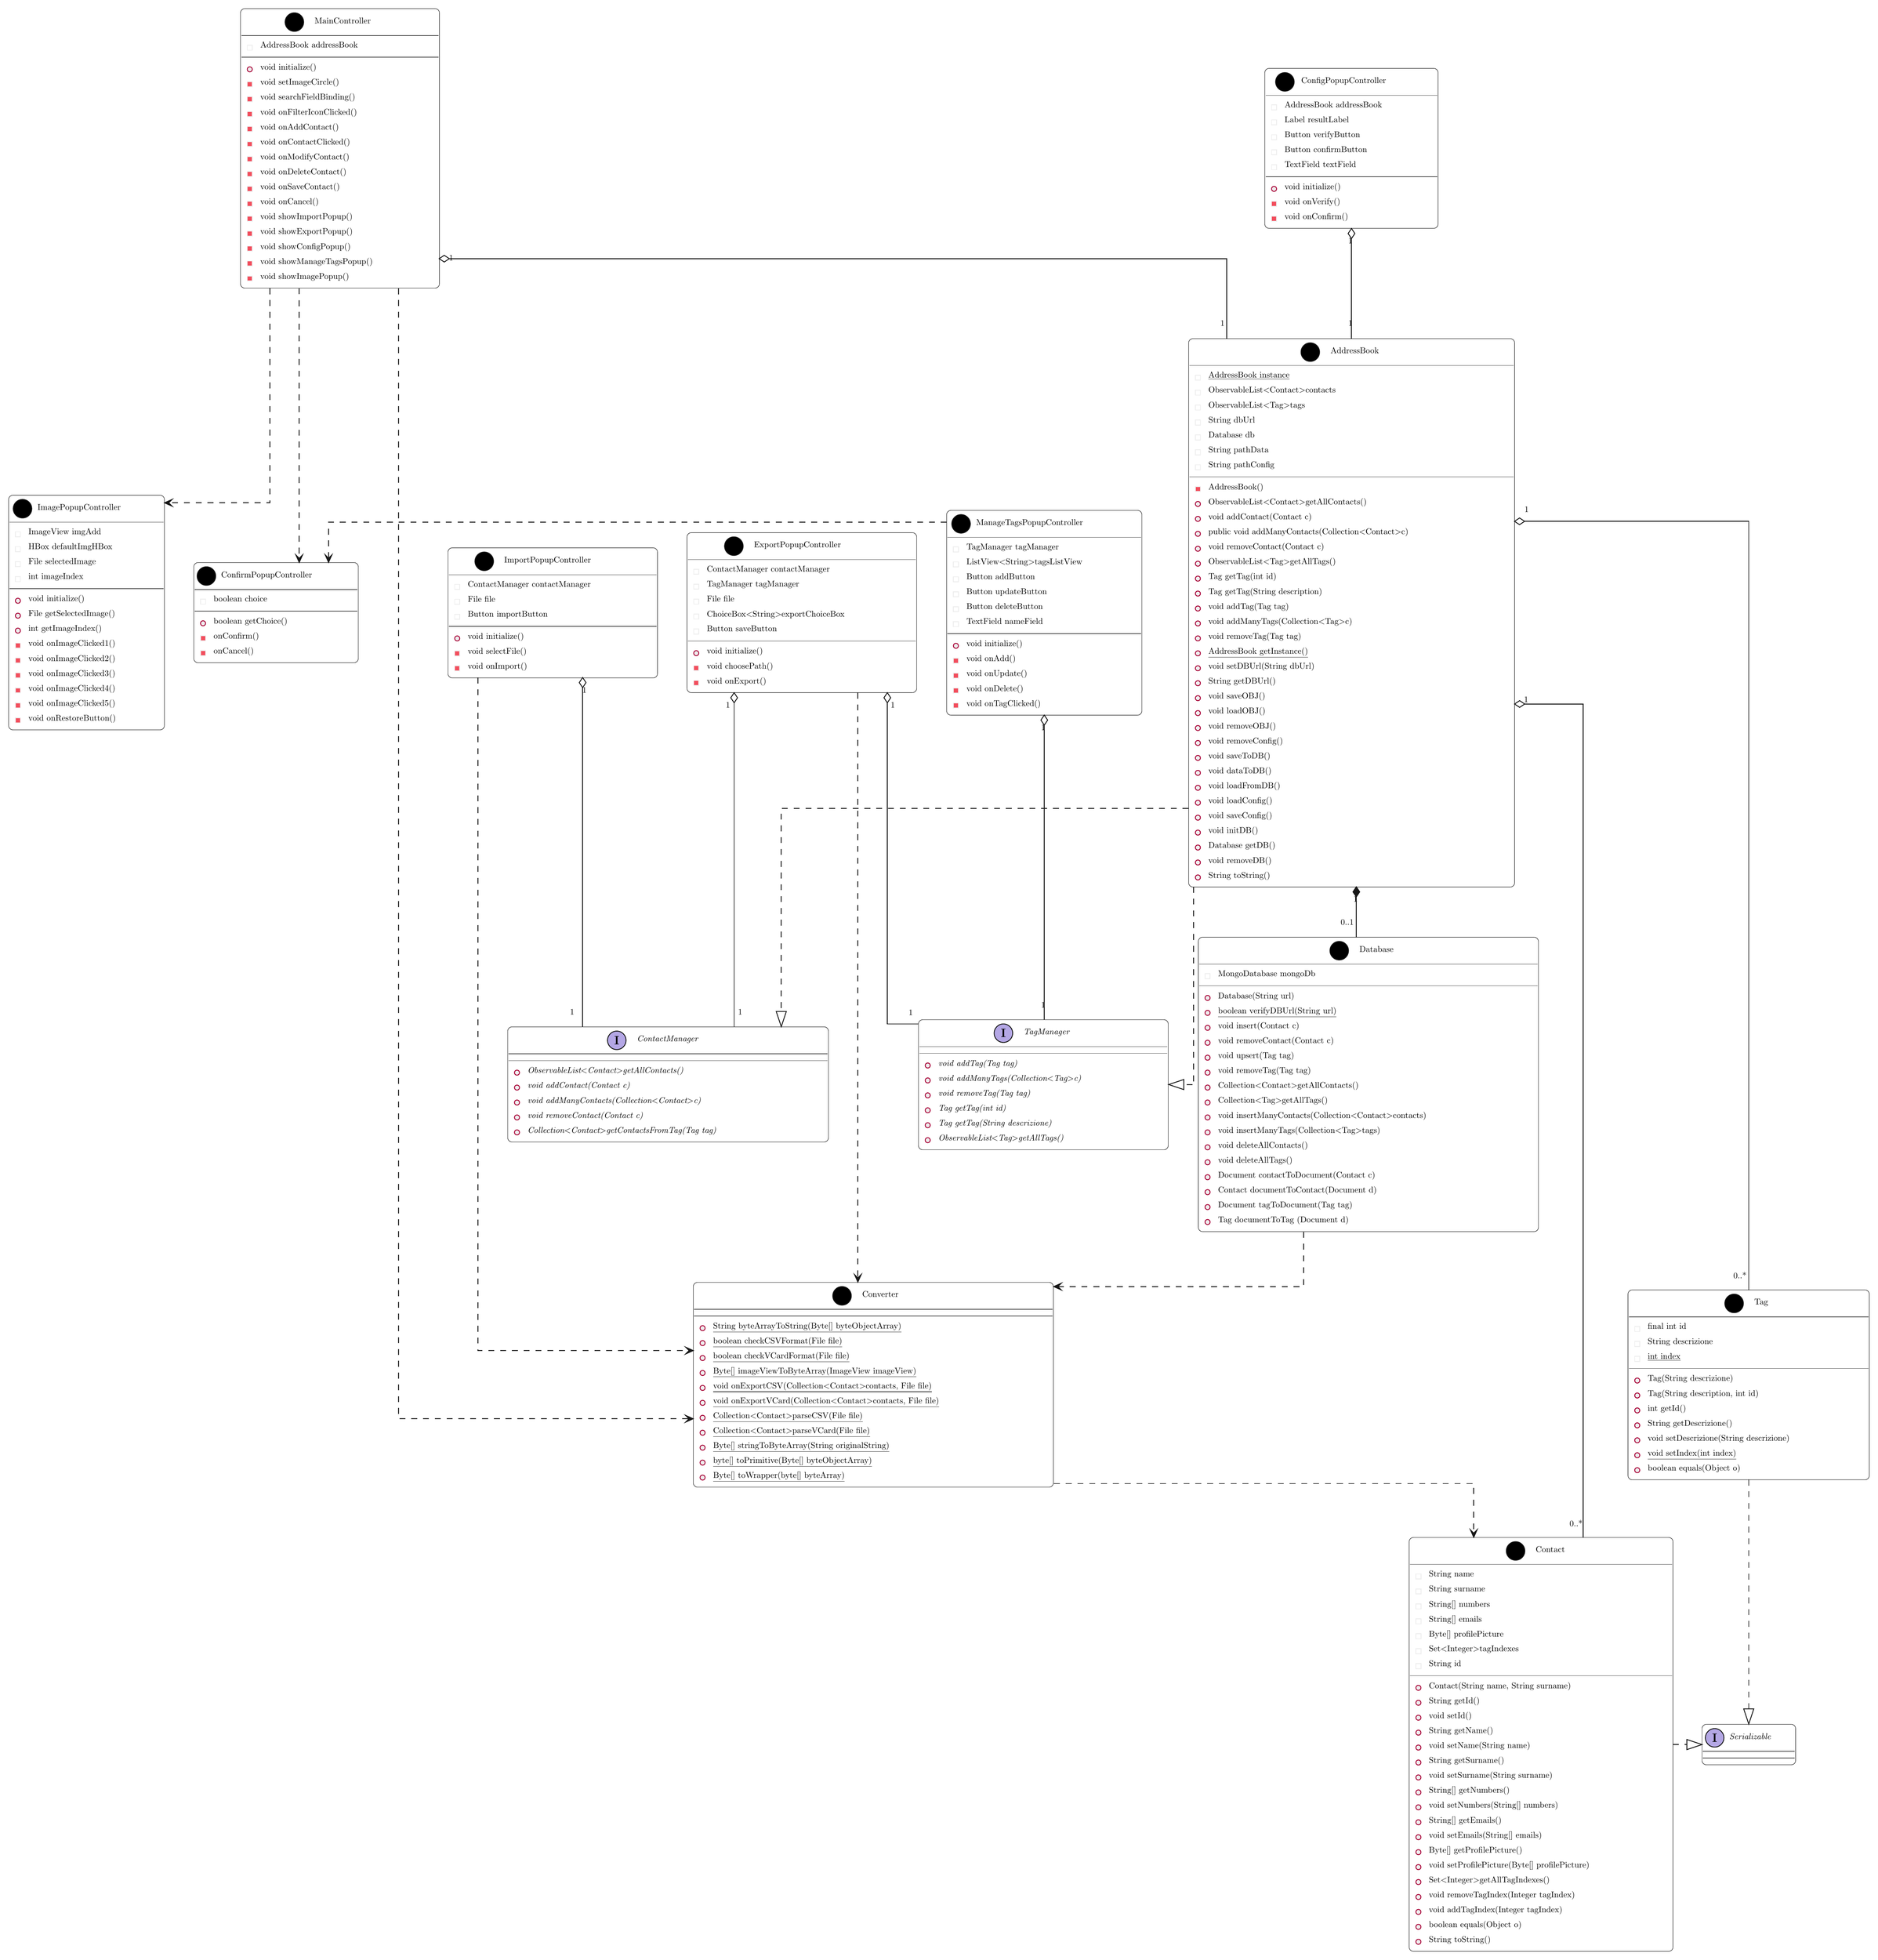
\begin{tikzpicture}[yscale=-1
,pstyle0/.style={color=plantucolor0001,fill=plantucolor0000,line width=0.5pt}
,pstyle1/.style={color=plantucolor0001,fill=plantucolor0002,line width=1.0pt}
,pstyle2/.style={color=plantucolor0001,line width=0.5pt}
,pstyle3/.style={color=plantucolor0004,line width=1.0pt}
,pstyle4/.style={color=plantucolor0006,fill=plantucolor0005,line width=1.0pt}
,pstyle5/.style={color=plantucolor0004,fill=plantucolor0007,line width=1.0pt}
,pstyle6/.style={color=plantucolor0001,fill=plantucolor0008,line width=1.0pt}
,pstyle7/.style={color=plantucolor0001,line width=1.0pt,dash pattern=on 7.0pt off 7.0pt}
,pstyle8/.style={color=plantucolor0001,line width=1.0pt}
,pstyle9/.style={color=plantucolor0001,fill=plantucolor0001,line width=1.0pt}
]
\draw[pstyle0] (1931pt,1534pt) arc (180:270:5pt) -- (1936pt,1529pt) -- (2212.7294pt,1529pt) arc (270:360:5pt) -- (2217.7294pt,1534pt) -- (2217.7294pt,1749.4609pt) arc (0:90:5pt) -- (2212.7294pt,1754.4609pt) -- (1936pt,1754.4609pt) arc (90:180:5pt) -- (1931pt,1749.4609pt) -- cycle;
\draw[pstyle1] (2057.0965pt,1545pt) ellipse (11pt and 11pt);
\node at (2057.0965pt,1545pt)[]{\textbf{\Large C}};
\node at (2077.5965pt,1536.127pt)[below right,color=black]{Tag};
\draw[pstyle2] (1932pt,1561pt) -- (2216.7294pt,1561pt);
\draw[pstyle3] (1939pt,1572.373pt) rectangle (1945pt,1578.373pt);
\node at (1951pt,1565pt)[below right,color=black]{final int id};
\draw[pstyle3] (1939pt,1590.1191pt) rectangle (1945pt,1596.1191pt);
\node at (1951pt,1582.7461pt)[below right,color=black]{String descrizione};
\draw[pstyle3] (1939pt,1607.8652pt) rectangle (1945pt,1613.8652pt);
\node at (1951pt,1600.4922pt)[below right,color=black]{\underline{int index}};
\draw[pstyle2] (1932pt,1622.2383pt) -- (2216.7294pt,1622.2383pt);
\draw[pstyle4] (1942pt,1636.6113pt) ellipse (3pt and 3pt);
\node at (1951pt,1626.2383pt)[below right,color=black]{Tag(String descrizione)};
\draw[pstyle4] (1942pt,1654.3574pt) ellipse (3pt and 3pt);
\node at (1951pt,1643.9844pt)[below right,color=black]{Tag(String description, int id)};
\draw[pstyle4] (1942pt,1672.1035pt) ellipse (3pt and 3pt);
\node at (1951pt,1661.7305pt)[below right,color=black]{int getId()};
\draw[pstyle4] (1942pt,1689.8496pt) ellipse (3pt and 3pt);
\node at (1951pt,1679.4766pt)[below right,color=black]{String getDescrizione()};
\draw[pstyle4] (1942pt,1707.5957pt) ellipse (3pt and 3pt);
\node at (1951pt,1697.2227pt)[below right,color=black]{void setDescrizione(String descrizione)};
\draw[pstyle4] (1942pt,1725.3418pt) ellipse (3pt and 3pt);
\node at (1951pt,1714.9688pt)[below right,color=black]{\underline{void setIndex(int index)}};
\draw[pstyle4] (1942pt,1743.0879pt) ellipse (3pt and 3pt);
\node at (1951pt,1732.7148pt)[below right,color=black]{boolean equals(Object o)};
\draw[pstyle0] (1671pt,1828pt) arc (180:270:5pt) -- (1676pt,1823pt) -- (1979.4602pt,1823pt) arc (270:360:5pt) -- (1984.4602pt,1828pt) -- (1984.4602pt,2309.6523pt) arc (0:90:5pt) -- (1979.4602pt,2314.6523pt) -- (1676pt,2314.6523pt) arc (90:180:5pt) -- (1671pt,2309.6523pt) -- cycle;
\draw[pstyle1] (1797.4437pt,1839pt) ellipse (11pt and 11pt);
\node at (1797.4437pt,1839pt)[]{\textbf{\Large C}};
\node at (1817.9437pt,1830.127pt)[below right,color=black]{Contact};
\draw[pstyle2] (1672pt,1855pt) -- (1983.4602pt,1855pt);
\draw[pstyle3] (1679pt,1866.373pt) rectangle (1685pt,1872.373pt);
\node at (1691pt,1859pt)[below right,color=black]{String name};
\draw[pstyle3] (1679pt,1884.1191pt) rectangle (1685pt,1890.1191pt);
\node at (1691pt,1876.7461pt)[below right,color=black]{String surname};
\draw[pstyle3] (1679pt,1901.8652pt) rectangle (1685pt,1907.8652pt);
\node at (1691pt,1894.4922pt)[below right,color=black]{String[] numbers};
\draw[pstyle3] (1679pt,1919.6113pt) rectangle (1685pt,1925.6113pt);
\node at (1691pt,1912.2383pt)[below right,color=black]{String[] emails};
\draw[pstyle3] (1679pt,1937.3574pt) rectangle (1685pt,1943.3574pt);
\node at (1691pt,1929.9844pt)[below right,color=black]{Byte[] profilePicture};
\draw[pstyle3] (1679pt,1955.1035pt) rectangle (1685pt,1961.1035pt);
\node at (1691pt,1947.7305pt)[below right,color=black]{Set\textless Integer\textgreater  tagIndexes};
\draw[pstyle3] (1679pt,1972.8496pt) rectangle (1685pt,1978.8496pt);
\node at (1691pt,1965.4766pt)[below right,color=black]{String id};
\draw[pstyle2] (1672pt,1987.2227pt) -- (1983.4602pt,1987.2227pt);
\draw[pstyle4] (1682pt,2001.5957pt) ellipse (3pt and 3pt);
\node at (1691pt,1991.2227pt)[below right,color=black]{Contact(String name, String surname)};
\draw[pstyle4] (1682pt,2019.3418pt) ellipse (3pt and 3pt);
\node at (1691pt,2008.9688pt)[below right,color=black]{String getId()};
\draw[pstyle4] (1682pt,2037.0879pt) ellipse (3pt and 3pt);
\node at (1691pt,2026.7148pt)[below right,color=black]{void setId()};
\draw[pstyle4] (1682pt,2054.834pt) ellipse (3pt and 3pt);
\node at (1691pt,2044.4609pt)[below right,color=black]{String getName()};
\draw[pstyle4] (1682pt,2072.5801pt) ellipse (3pt and 3pt);
\node at (1691pt,2062.207pt)[below right,color=black]{void setName(String name)};
\draw[pstyle4] (1682pt,2090.3262pt) ellipse (3pt and 3pt);
\node at (1691pt,2079.9531pt)[below right,color=black]{String getSurname()};
\draw[pstyle4] (1682pt,2108.0723pt) ellipse (3pt and 3pt);
\node at (1691pt,2097.6992pt)[below right,color=black]{void setSurname(String surname)};
\draw[pstyle4] (1682pt,2125.8184pt) ellipse (3pt and 3pt);
\node at (1691pt,2115.4453pt)[below right,color=black]{String[] getNumbers()};
\draw[pstyle4] (1682pt,2143.5645pt) ellipse (3pt and 3pt);
\node at (1691pt,2133.1914pt)[below right,color=black]{void setNumbers(String[] numbers)};
\draw[pstyle4] (1682pt,2161.3105pt) ellipse (3pt and 3pt);
\node at (1691pt,2150.9375pt)[below right,color=black]{String[] getEmails()};
\draw[pstyle4] (1682pt,2179.0566pt) ellipse (3pt and 3pt);
\node at (1691pt,2168.6836pt)[below right,color=black]{void setEmails(String[] emails)};
\draw[pstyle4] (1682pt,2196.8027pt) ellipse (3pt and 3pt);
\node at (1691pt,2186.4297pt)[below right,color=black]{Byte[] getProfilePicture()};
\draw[pstyle4] (1682pt,2214.5488pt) ellipse (3pt and 3pt);
\node at (1691pt,2204.1758pt)[below right,color=black]{void setProfilePicture(Byte[] profilePicture)};
\draw[pstyle4] (1682pt,2232.2949pt) ellipse (3pt and 3pt);
\node at (1691pt,2221.9219pt)[below right,color=black]{Set\textless Integer\textgreater  getAllTagIndexes()};
\draw[pstyle4] (1682pt,2250.041pt) ellipse (3pt and 3pt);
\node at (1691pt,2239.668pt)[below right,color=black]{void removeTagIndex(Integer tagIndex)};
\draw[pstyle4] (1682pt,2267.7871pt) ellipse (3pt and 3pt);
\node at (1691pt,2257.4141pt)[below right,color=black]{void addTagIndex(Integer tagIndex)};
\draw[pstyle4] (1682pt,2285.5332pt) ellipse (3pt and 3pt);
\node at (1691pt,2275.1602pt)[below right,color=black]{boolean equals(Object o)};
\draw[pstyle4] (1682pt,2303.2793pt) ellipse (3pt and 3pt);
\node at (1691pt,2292.9063pt)[below right,color=black]{String toString()};
\draw[pstyle0] (1409pt,404pt) arc (180:270:5pt) -- (1414pt,399pt) -- (1791.2787pt,399pt) arc (270:360:5pt) -- (1796.2787pt,404pt) -- (1796.2787pt,1045.3672pt) arc (0:90:5pt) -- (1791.2787pt,1050.3672pt) -- (1414pt,1050.3672pt) arc (90:180:5pt) -- (1409pt,1045.3672pt) -- cycle;
\draw[pstyle1] (1553.5493pt,415pt) ellipse (11pt and 11pt);
\node at (1553.5493pt,415pt)[]{\textbf{\Large C}};
\node at (1574.0493pt,406.127pt)[below right,color=black]{AddressBook};
\draw[pstyle2] (1410pt,431pt) -- (1795.2787pt,431pt);
\draw[pstyle3] (1417pt,442.373pt) rectangle (1423pt,448.373pt);
\node at (1429pt,435pt)[below right,color=black]{\underline{AddressBook instance}};
\draw[pstyle3] (1417pt,460.1191pt) rectangle (1423pt,466.1191pt);
\node at (1429pt,452.7461pt)[below right,color=black]{ObservableList\textless Contact\textgreater  contacts};
\draw[pstyle3] (1417pt,477.8652pt) rectangle (1423pt,483.8652pt);
\node at (1429pt,470.4922pt)[below right,color=black]{ObservableList\textless Tag\textgreater  tags};
\draw[pstyle3] (1417pt,495.6113pt) rectangle (1423pt,501.6113pt);
\node at (1429pt,488.2383pt)[below right,color=black]{String dbUrl};
\draw[pstyle3] (1417pt,513.3574pt) rectangle (1423pt,519.3574pt);
\node at (1429pt,505.9844pt)[below right,color=black]{Database db};
\draw[pstyle3] (1417pt,531.1035pt) rectangle (1423pt,537.1035pt);
\node at (1429pt,523.7305pt)[below right,color=black]{String pathData};
\draw[pstyle3] (1417pt,548.8496pt) rectangle (1423pt,554.8496pt);
\node at (1429pt,541.4766pt)[below right,color=black]{String pathConfig};
\draw[pstyle2] (1410pt,563.2227pt) -- (1795.2787pt,563.2227pt);
\draw[pstyle5] (1417pt,574.5957pt) rectangle (1423pt,580.5957pt);
\node at (1429pt,567.2227pt)[below right,color=black]{AddressBook()};
\draw[pstyle4] (1420pt,595.3418pt) ellipse (3pt and 3pt);
\node at (1429pt,584.9688pt)[below right,color=black]{ObservableList\textless Contact\textgreater  getAllContacts()};
\draw[pstyle4] (1420pt,613.0879pt) ellipse (3pt and 3pt);
\node at (1429pt,602.7148pt)[below right,color=black]{void addContact(Contact c)};
\draw[pstyle4] (1420pt,630.834pt) ellipse (3pt and 3pt);
\node at (1429pt,620.4609pt)[below right,color=black]{public void addManyContacts(Collection\textless Contact\textgreater  c)};
\draw[pstyle4] (1420pt,648.5801pt) ellipse (3pt and 3pt);
\node at (1429pt,638.207pt)[below right,color=black]{void removeContact(Contact c)};
\draw[pstyle4] (1420pt,666.3262pt) ellipse (3pt and 3pt);
\node at (1429pt,655.9531pt)[below right,color=black]{ObservableList\textless Tag\textgreater  getAllTags()};
\draw[pstyle4] (1420pt,684.0723pt) ellipse (3pt and 3pt);
\node at (1429pt,673.6992pt)[below right,color=black]{Tag getTag(int id)};
\draw[pstyle4] (1420pt,701.8184pt) ellipse (3pt and 3pt);
\node at (1429pt,691.4453pt)[below right,color=black]{Tag getTag(String description)};
\draw[pstyle4] (1420pt,719.5645pt) ellipse (3pt and 3pt);
\node at (1429pt,709.1914pt)[below right,color=black]{void addTag(Tag tag)};
\draw[pstyle4] (1420pt,737.3105pt) ellipse (3pt and 3pt);
\node at (1429pt,726.9375pt)[below right,color=black]{void addManyTags(Collection\textless Tag\textgreater  c)};
\draw[pstyle4] (1420pt,755.0566pt) ellipse (3pt and 3pt);
\node at (1429pt,744.6836pt)[below right,color=black]{void removeTag(Tag tag)};
\draw[pstyle4] (1420pt,772.8027pt) ellipse (3pt and 3pt);
\node at (1429pt,762.4297pt)[below right,color=black]{\underline{AddressBook getInstance()}};
\draw[pstyle4] (1420pt,790.5488pt) ellipse (3pt and 3pt);
\node at (1429pt,780.1758pt)[below right,color=black]{void setDBUrl(String dbUrl)};
\draw[pstyle4] (1420pt,808.2949pt) ellipse (3pt and 3pt);
\node at (1429pt,797.9219pt)[below right,color=black]{String getDBUrl()};
\draw[pstyle4] (1420pt,826.041pt) ellipse (3pt and 3pt);
\node at (1429pt,815.668pt)[below right,color=black]{void saveOBJ()};
\draw[pstyle4] (1420pt,843.7871pt) ellipse (3pt and 3pt);
\node at (1429pt,833.4141pt)[below right,color=black]{void loadOBJ()};
\draw[pstyle4] (1420pt,861.5332pt) ellipse (3pt and 3pt);
\node at (1429pt,851.1602pt)[below right,color=black]{void removeOBJ()};
\draw[pstyle4] (1420pt,879.2793pt) ellipse (3pt and 3pt);
\node at (1429pt,868.9063pt)[below right,color=black]{void removeConfig()};
\draw[pstyle4] (1420pt,897.0254pt) ellipse (3pt and 3pt);
\node at (1429pt,886.6523pt)[below right,color=black]{void saveToDB()};
\draw[pstyle4] (1420pt,914.7715pt) ellipse (3pt and 3pt);
\node at (1429pt,904.3984pt)[below right,color=black]{void dataToDB()};
\draw[pstyle4] (1420pt,932.5176pt) ellipse (3pt and 3pt);
\node at (1429pt,922.1445pt)[below right,color=black]{void loadFromDB()};
\draw[pstyle4] (1420pt,950.2637pt) ellipse (3pt and 3pt);
\node at (1429pt,939.8906pt)[below right,color=black]{void loadConfig()};
\draw[pstyle4] (1420pt,968.0098pt) ellipse (3pt and 3pt);
\node at (1429pt,957.6367pt)[below right,color=black]{void saveConfig()};
\draw[pstyle4] (1420pt,985.7559pt) ellipse (3pt and 3pt);
\node at (1429pt,975.3828pt)[below right,color=black]{void initDB()};
\draw[pstyle4] (1420pt,1003.502pt) ellipse (3pt and 3pt);
\node at (1429pt,993.1289pt)[below right,color=black]{Database getDB()};
\draw[pstyle4] (1420pt,1021.248pt) ellipse (3pt and 3pt);
\node at (1429pt,1010.875pt)[below right,color=black]{void removeDB()};
\draw[pstyle4] (1420pt,1038.9941pt) ellipse (3pt and 3pt);
\node at (1429pt,1028.6211pt)[below right,color=black]{String toString()};
\draw[pstyle0] (282.5pt,12pt) arc (180:270:5pt) -- (287.5pt,7pt) -- (513.8435pt,7pt) arc (270:360:5pt) -- (518.8435pt,12pt) -- (518.8435pt,333.9375pt) arc (0:90:5pt) -- (513.8435pt,338.9375pt) -- (287.5pt,338.9375pt) arc (90:180:5pt) -- (282.5pt,333.9375pt) -- cycle;
\draw[pstyle1] (346.5218pt,23pt) ellipse (11pt and 11pt);
\node at (346.5218pt,23pt)[]{\textbf{\Large C}};
\node at (367.0218pt,14.127pt)[below right,color=black]{MainController};
\draw[pstyle2] (283.5pt,39pt) -- (517.8435pt,39pt);
\draw[pstyle3] (290.5pt,50.373pt) rectangle (296.5pt,56.373pt);
\node at (302.5pt,43pt)[below right,color=black]{AddressBook addressBook};
\draw[pstyle2] (283.5pt,64.7461pt) -- (517.8435pt,64.7461pt);
\draw[pstyle4] (293.5pt,79.1191pt) ellipse (3pt and 3pt);
\node at (302.5pt,68.7461pt)[below right,color=black]{void initialize()};
\draw[pstyle5] (290.5pt,93.8652pt) rectangle (296.5pt,99.8652pt);
\node at (302.5pt,86.4922pt)[below right,color=black]{void setImageCircle()};
\draw[pstyle5] (290.5pt,111.6113pt) rectangle (296.5pt,117.6113pt);
\node at (302.5pt,104.2383pt)[below right,color=black]{void searchFieldBinding()};
\draw[pstyle5] (290.5pt,129.3574pt) rectangle (296.5pt,135.3574pt);
\node at (302.5pt,121.9844pt)[below right,color=black]{void onFilterIconClicked()};
\draw[pstyle5] (290.5pt,147.1035pt) rectangle (296.5pt,153.1035pt);
\node at (302.5pt,139.7305pt)[below right,color=black]{void onAddContact()};
\draw[pstyle5] (290.5pt,164.8496pt) rectangle (296.5pt,170.8496pt);
\node at (302.5pt,157.4766pt)[below right,color=black]{void onContactClicked()};
\draw[pstyle5] (290.5pt,182.5957pt) rectangle (296.5pt,188.5957pt);
\node at (302.5pt,175.2227pt)[below right,color=black]{void onModifyContact()};
\draw[pstyle5] (290.5pt,200.3418pt) rectangle (296.5pt,206.3418pt);
\node at (302.5pt,192.9688pt)[below right,color=black]{void onDeleteContact()};
\draw[pstyle5] (290.5pt,218.0879pt) rectangle (296.5pt,224.0879pt);
\node at (302.5pt,210.7148pt)[below right,color=black]{void onSaveContact()};
\draw[pstyle5] (290.5pt,235.834pt) rectangle (296.5pt,241.834pt);
\node at (302.5pt,228.4609pt)[below right,color=black]{void onCancel()};
\draw[pstyle5] (290.5pt,253.5801pt) rectangle (296.5pt,259.5801pt);
\node at (302.5pt,246.207pt)[below right,color=black]{void showImportPopup()};
\draw[pstyle5] (290.5pt,271.3262pt) rectangle (296.5pt,277.3262pt);
\node at (302.5pt,263.9531pt)[below right,color=black]{void showExportPopup()};
\draw[pstyle5] (290.5pt,289.0723pt) rectangle (296.5pt,295.0723pt);
\node at (302.5pt,281.6992pt)[below right,color=black]{void showConfigPopup()};
\draw[pstyle5] (290.5pt,306.8184pt) rectangle (296.5pt,312.8184pt);
\node at (302.5pt,299.4453pt)[below right,color=black]{void showManageTagsPopup()};
\draw[pstyle5] (290.5pt,324.5645pt) rectangle (296.5pt,330.5645pt);
\node at (302.5pt,317.1914pt)[below right,color=black]{void showImagePopup()};
\draw[pstyle0] (820.5pt,1525pt) arc (180:270:5pt) -- (825.5pt,1520pt) -- (1243.3041pt,1520pt) arc (270:360:5pt) -- (1248.3041pt,1525pt) -- (1248.3041pt,1758.207pt) arc (0:90:5pt) -- (1243.3041pt,1763.207pt) -- (825.5pt,1763.207pt) arc (90:180:5pt) -- (820.5pt,1758.207pt) -- cycle;
\draw[pstyle1] (997.1949pt,1536pt) ellipse (11pt and 11pt);
\node at (997.1949pt,1536pt)[]{\textbf{\Large C}};
\node at (1017.6949pt,1527.127pt)[below right,color=black]{Converter};
\draw[pstyle2] (821.5pt,1552pt) -- (1247.3041pt,1552pt);
\draw[pstyle2] (821.5pt,1560pt) -- (1247.3041pt,1560pt);
\draw[pstyle4] (831.5pt,1574.373pt) ellipse (3pt and 3pt);
\node at (840.5pt,1564pt)[below right,color=black]{\underline{String byteArrayToString(Byte[] byteObjectArray)}};
\draw[pstyle4] (831.5pt,1592.1191pt) ellipse (3pt and 3pt);
\node at (840.5pt,1581.7461pt)[below right,color=black]{\underline{boolean checkCSVFormat(File file)}};
\draw[pstyle4] (831.5pt,1609.8652pt) ellipse (3pt and 3pt);
\node at (840.5pt,1599.4922pt)[below right,color=black]{\underline{boolean checkVCardFormat(File file)}};
\draw[pstyle4] (831.5pt,1627.6113pt) ellipse (3pt and 3pt);
\node at (840.5pt,1617.2383pt)[below right,color=black]{\underline{Byte[] imageViewToByteArray(ImageView imageView)}};
\draw[pstyle4] (831.5pt,1645.3574pt) ellipse (3pt and 3pt);
\node at (840.5pt,1634.9844pt)[below right,color=black]{\underline{void onExportCSV(Collection\textless Contact\textgreater  contacts, File file)}};
\draw[pstyle4] (831.5pt,1663.1035pt) ellipse (3pt and 3pt);
\node at (840.5pt,1652.7305pt)[below right,color=black]{\underline{void onExportVCard(Collection\textless Contact\textgreater  contacts, File file)}};
\draw[pstyle4] (831.5pt,1680.8496pt) ellipse (3pt and 3pt);
\node at (840.5pt,1670.4766pt)[below right,color=black]{\underline{Collection\textless Contact\textgreater  parseCSV(File file)}};
\draw[pstyle4] (831.5pt,1698.5957pt) ellipse (3pt and 3pt);
\node at (840.5pt,1688.2227pt)[below right,color=black]{\underline{Collection\textless Contact\textgreater  parseVCard(File file)}};
\draw[pstyle4] (831.5pt,1716.3418pt) ellipse (3pt and 3pt);
\node at (840.5pt,1705.9688pt)[below right,color=black]{\underline{Byte[] stringToByteArray(String originalString)}};
\draw[pstyle4] (831.5pt,1734.0879pt) ellipse (3pt and 3pt);
\node at (840.5pt,1723.7148pt)[below right,color=black]{\underline{byte[] toPrimitive(Byte[] byteObjectArray)}};
\draw[pstyle4] (831.5pt,1751.834pt) ellipse (3pt and 3pt);
\node at (840.5pt,1741.4609pt)[below right,color=black]{\underline{Byte[] toWrapper(byte[] byteArray)}};
\draw[pstyle0] (529pt,652.5pt) arc (180:270:5pt) -- (534pt,647.5pt) -- (772.9191pt,647.5pt) arc (270:360:5pt) -- (777.9191pt,652.5pt) -- (777.9191pt,796.9766pt) arc (0:90:5pt) -- (772.9191pt,801.9766pt) -- (534pt,801.9766pt) arc (90:180:5pt) -- (529pt,796.9766pt) -- cycle;
\draw[pstyle1] (572.0828pt,663.5pt) ellipse (11pt and 11pt);
\node at (572.0828pt,663.5pt)[]{\textbf{\Large C}};
\node at (592.3234pt,654.627pt)[below right,color=black]{ImportPopupController};
\draw[pstyle2] (530pt,679.5pt) -- (776.9191pt,679.5pt);
\draw[pstyle3] (537pt,690.873pt) rectangle (543pt,696.873pt);
\node at (549pt,683.5pt)[below right,color=black]{ContactManager contactManager};
\draw[pstyle3] (537pt,708.6191pt) rectangle (543pt,714.6191pt);
\node at (549pt,701.2461pt)[below right,color=black]{File file};
\draw[pstyle3] (537pt,726.3652pt) rectangle (543pt,732.3652pt);
\node at (549pt,718.9922pt)[below right,color=black]{Button importButton};
\draw[pstyle2] (530pt,740.7383pt) -- (776.9191pt,740.7383pt);
\draw[pstyle4] (540pt,755.1113pt) ellipse (3pt and 3pt);
\node at (549pt,744.7383pt)[below right,color=black]{void initialize()};
\draw[pstyle5] (537pt,769.8574pt) rectangle (543pt,775.8574pt);
\node at (549pt,762.4844pt)[below right,color=black]{void selectFile()};
\draw[pstyle5] (537pt,787.6035pt) rectangle (543pt,793.6035pt);
\node at (549pt,780.2305pt)[below right,color=black]{void onImport()};
\draw[pstyle0] (813pt,634.5pt) arc (180:270:5pt) -- (818pt,629.5pt) -- (1080.8528pt,629.5pt) arc (270:360:5pt) -- (1085.8528pt,634.5pt) -- (1085.8528pt,814.4688pt) arc (0:90:5pt) -- (1080.8528pt,819.4688pt) -- (818pt,819.4688pt) arc (90:180:5pt) -- (813pt,814.4688pt) -- cycle;
\draw[pstyle1] (868.6533pt,645.5pt) ellipse (11pt and 11pt);
\node at (868.6533pt,645.5pt)[]{\textbf{\Large C}};
\node at (889.1533pt,636.627pt)[below right,color=black]{ExportPopupController};
\draw[pstyle2] (814pt,661.5pt) -- (1084.8528pt,661.5pt);
\draw[pstyle3] (821pt,672.873pt) rectangle (827pt,678.873pt);
\node at (833pt,665.5pt)[below right,color=black]{ContactManager contactManager};
\draw[pstyle3] (821pt,690.6191pt) rectangle (827pt,696.6191pt);
\node at (833pt,683.2461pt)[below right,color=black]{TagManager tagManager};
\draw[pstyle3] (821pt,708.3652pt) rectangle (827pt,714.3652pt);
\node at (833pt,700.9922pt)[below right,color=black]{File file};
\draw[pstyle3] (821pt,726.1113pt) rectangle (827pt,732.1113pt);
\node at (833pt,718.7383pt)[below right,color=black]{ChoiceBox\textless String\textgreater  exportChoiceBox};
\draw[pstyle3] (821pt,743.8574pt) rectangle (827pt,749.8574pt);
\node at (833pt,736.4844pt)[below right,color=black]{Button saveButton};
\draw[pstyle2] (814pt,758.2305pt) -- (1084.8528pt,758.2305pt);
\draw[pstyle4] (824pt,772.6035pt) ellipse (3pt and 3pt);
\node at (833pt,762.2305pt)[below right,color=black]{void initialize()};
\draw[pstyle5] (821pt,787.3496pt) rectangle (827pt,793.3496pt);
\node at (833pt,779.9766pt)[below right,color=black]{void choosePath()};
\draw[pstyle5] (821pt,805.0957pt) rectangle (827pt,811.0957pt);
\node at (833pt,797.7227pt)[below right,color=black]{void onExport()};
\draw[pstyle0] (1121.5pt,608pt) arc (180:270:5pt) -- (1126.5pt,603pt) -- (1348.4367pt,603pt) arc (270:360:5pt) -- (1353.4367pt,608pt) -- (1353.4367pt,841.207pt) arc (0:90:5pt) -- (1348.4367pt,846.207pt) -- (1126.5pt,846.207pt) arc (90:180:5pt) -- (1121.5pt,841.207pt) -- cycle;
\draw[pstyle1] (1138.6249pt,619pt) ellipse (11pt and 11pt);
\node at (1138.6249pt,619pt)[]{\textbf{\Large C}};
\node at (1153.0971pt,610.127pt)[below right,color=black]{ManageTagsPopupController};
\draw[pstyle2] (1122.5pt,635pt) -- (1352.4367pt,635pt);
\draw[pstyle3] (1129.5pt,646.373pt) rectangle (1135.5pt,652.373pt);
\node at (1141.5pt,639pt)[below right,color=black]{TagManager tagManager};
\draw[pstyle3] (1129.5pt,664.1191pt) rectangle (1135.5pt,670.1191pt);
\node at (1141.5pt,656.7461pt)[below right,color=black]{ListView\textless String\textgreater  tagsListView};
\draw[pstyle3] (1129.5pt,681.8652pt) rectangle (1135.5pt,687.8652pt);
\node at (1141.5pt,674.4922pt)[below right,color=black]{Button addButton};
\draw[pstyle3] (1129.5pt,699.6113pt) rectangle (1135.5pt,705.6113pt);
\node at (1141.5pt,692.2383pt)[below right,color=black]{Button updateButton};
\draw[pstyle3] (1129.5pt,717.3574pt) rectangle (1135.5pt,723.3574pt);
\node at (1141.5pt,709.9844pt)[below right,color=black]{Button deleteButton};
\draw[pstyle3] (1129.5pt,735.1035pt) rectangle (1135.5pt,741.1035pt);
\node at (1141.5pt,727.7305pt)[below right,color=black]{TextField nameField};
\draw[pstyle2] (1122.5pt,749.4766pt) -- (1352.4367pt,749.4766pt);
\draw[pstyle4] (1132.5pt,763.8496pt) ellipse (3pt and 3pt);
\node at (1141.5pt,753.4766pt)[below right,color=black]{void initialize()};
\draw[pstyle5] (1129.5pt,778.5957pt) rectangle (1135.5pt,784.5957pt);
\node at (1141.5pt,771.2227pt)[below right,color=black]{void onAdd()};
\draw[pstyle5] (1129.5pt,796.3418pt) rectangle (1135.5pt,802.3418pt);
\node at (1141.5pt,788.9688pt)[below right,color=black]{void onUpdate()};
\draw[pstyle5] (1129.5pt,814.0879pt) rectangle (1135.5pt,820.0879pt);
\node at (1141.5pt,806.7148pt)[below right,color=black]{void onDelete()};
\draw[pstyle5] (1129.5pt,831.834pt) rectangle (1135.5pt,837.834pt);
\node at (1141.5pt,824.4609pt)[below right,color=black]{void onTagClicked()};
\draw[pstyle0] (7pt,590pt) arc (180:270:5pt) -- (12pt,585pt) -- (187.0824pt,585pt) arc (270:360:5pt) -- (192.0824pt,590pt) -- (192.0824pt,858.6992pt) arc (0:90:5pt) -- (187.0824pt,863.6992pt) -- (12pt,863.6992pt) arc (90:180:5pt) -- (7pt,858.6992pt) -- cycle;
\draw[pstyle1] (23.4976pt,601pt) ellipse (11pt and 11pt);
\node at (23.4976pt,601pt)[]{\textbf{\Large C}};
\node at (37.8304pt,592.127pt)[below right,color=black]{ImagePopupController};
\draw[pstyle2] (8pt,617pt) -- (191.0824pt,617pt);
\draw[pstyle3] (15pt,628.373pt) rectangle (21pt,634.373pt);
\node at (27pt,621pt)[below right,color=black]{ImageView imgAdd};
\draw[pstyle3] (15pt,646.1191pt) rectangle (21pt,652.1191pt);
\node at (27pt,638.7461pt)[below right,color=black]{HBox defaultImgHBox};
\draw[pstyle3] (15pt,663.8652pt) rectangle (21pt,669.8652pt);
\node at (27pt,656.4922pt)[below right,color=black]{File selectedImage};
\draw[pstyle3] (15pt,681.6113pt) rectangle (21pt,687.6113pt);
\node at (27pt,674.2383pt)[below right,color=black]{int imageIndex};
\draw[pstyle2] (8pt,695.9844pt) -- (191.0824pt,695.9844pt);
\draw[pstyle4] (18pt,710.3574pt) ellipse (3pt and 3pt);
\node at (27pt,699.9844pt)[below right,color=black]{void initialize()};
\draw[pstyle4] (18pt,728.1035pt) ellipse (3pt and 3pt);
\node at (27pt,717.7305pt)[below right,color=black]{File getSelectedImage()};
\draw[pstyle4] (18pt,745.8496pt) ellipse (3pt and 3pt);
\node at (27pt,735.4766pt)[below right,color=black]{int getImageIndex()};
\draw[pstyle5] (15pt,760.5957pt) rectangle (21pt,766.5957pt);
\node at (27pt,753.2227pt)[below right,color=black]{void onImageClicked1()};
\draw[pstyle5] (15pt,778.3418pt) rectangle (21pt,784.3418pt);
\node at (27pt,770.9688pt)[below right,color=black]{void onImageClicked2()};
\draw[pstyle5] (15pt,796.0879pt) rectangle (21pt,802.0879pt);
\node at (27pt,788.7148pt)[below right,color=black]{void onImageClicked3()};
\draw[pstyle5] (15pt,813.834pt) rectangle (21pt,819.834pt);
\node at (27pt,806.4609pt)[below right,color=black]{void onImageClicked4()};
\draw[pstyle5] (15pt,831.5801pt) rectangle (21pt,837.5801pt);
\node at (27pt,824.207pt)[below right,color=black]{void onImageClicked5()};
\draw[pstyle5] (15pt,849.3262pt) rectangle (21pt,855.3262pt);
\node at (27pt,841.9531pt)[below right,color=black]{void onRestoreButton()};
\draw[pstyle0] (227pt,670pt) arc (180:270:5pt) -- (232pt,665pt) -- (417.4331pt,665pt) arc (270:360:5pt) -- (422.4331pt,670pt) -- (422.4331pt,778.9844pt) arc (0:90:5pt) -- (417.4331pt,783.9844pt) -- (232pt,783.9844pt) arc (90:180:5pt) -- (227pt,778.9844pt) -- cycle;
\draw[pstyle1] (242pt,681pt) ellipse (11pt and 11pt);
\node at (242pt,681pt)[]{\textbf{\Large C}};
\node at (256pt,672.127pt)[below right,color=black]{ConfirmPopupController};
\draw[pstyle2] (228pt,697pt) -- (421.4331pt,697pt);
\draw[pstyle3] (235pt,708.373pt) rectangle (241pt,714.373pt);
\node at (247pt,701pt)[below right,color=black]{boolean choice};
\draw[pstyle2] (228pt,722.7461pt) -- (421.4331pt,722.7461pt);
\draw[pstyle4] (238pt,737.1191pt) ellipse (3pt and 3pt);
\node at (247pt,726.7461pt)[below right,color=black]{boolean getChoice()};
\draw[pstyle5] (235pt,751.8652pt) rectangle (241pt,757.8652pt);
\node at (247pt,744.4922pt)[below right,color=black]{onConfirm()};
\draw[pstyle5] (235pt,769.6113pt) rectangle (241pt,775.6113pt);
\node at (247pt,762.2383pt)[below right,color=black]{onCancel()};
\draw[pstyle0] (1499.5pt,83pt) arc (180:270:5pt) -- (1504.5pt,78pt) -- (1700.3225pt,78pt) arc (270:360:5pt) -- (1705.3225pt,83pt) -- (1705.3225pt,262.9688pt) arc (0:90:5pt) -- (1700.3225pt,267.9688pt) -- (1504.5pt,267.9688pt) arc (90:180:5pt) -- (1499.5pt,262.9688pt) -- cycle;
\draw[pstyle1] (1523.3509pt,94pt) ellipse (11pt and 11pt);
\node at (1523.3509pt,94pt)[]{\textbf{\Large C}};
\node at (1539.3178pt,85.127pt)[below right,color=black]{ConfigPopupController};
\draw[pstyle2] (1500.5pt,110pt) -- (1704.3225pt,110pt);
\draw[pstyle3] (1507.5pt,121.373pt) rectangle (1513.5pt,127.373pt);
\node at (1519.5pt,114pt)[below right,color=black]{AddressBook addressBook};
\draw[pstyle3] (1507.5pt,139.1191pt) rectangle (1513.5pt,145.1191pt);
\node at (1519.5pt,131.7461pt)[below right,color=black]{Label resultLabel};
\draw[pstyle3] (1507.5pt,156.8652pt) rectangle (1513.5pt,162.8652pt);
\node at (1519.5pt,149.4922pt)[below right,color=black]{Button verifyButton};
\draw[pstyle3] (1507.5pt,174.6113pt) rectangle (1513.5pt,180.6113pt);
\node at (1519.5pt,167.2383pt)[below right,color=black]{Button confirmButton};
\draw[pstyle3] (1507.5pt,192.3574pt) rectangle (1513.5pt,198.3574pt);
\node at (1519.5pt,184.9844pt)[below right,color=black]{TextField textField};
\draw[pstyle2] (1500.5pt,206.7305pt) -- (1704.3225pt,206.7305pt);
\draw[pstyle4] (1510.5pt,221.1035pt) ellipse (3pt and 3pt);
\node at (1519.5pt,210.7305pt)[below right,color=black]{void initialize()};
\draw[pstyle5] (1507.5pt,235.8496pt) rectangle (1513.5pt,241.8496pt);
\node at (1519.5pt,228.4766pt)[below right,color=black]{void onVerify()};
\draw[pstyle5] (1507.5pt,253.5957pt) rectangle (1513.5pt,259.5957pt);
\node at (1519.5pt,246.2227pt)[below right,color=black]{void onConfirm()};
\draw[pstyle0] (1420.5pt,1115pt) arc (180:270:5pt) -- (1425.5pt,1110pt) -- (1819.5978pt,1110pt) arc (270:360:5pt) -- (1824.5978pt,1115pt) -- (1824.5978pt,1454.6836pt) arc (0:90:5pt) -- (1819.5978pt,1459.6836pt) -- (1425.5pt,1459.6836pt) arc (90:180:5pt) -- (1420.5pt,1454.6836pt) -- cycle;
\draw[pstyle1] (1587.9342pt,1126pt) ellipse (11pt and 11pt);
\node at (1587.9342pt,1126pt)[]{\textbf{\Large C}};
\node at (1608.4342pt,1117.127pt)[below right,color=black]{Database};
\draw[pstyle2] (1421.5pt,1142pt) -- (1823.5978pt,1142pt);
\draw[pstyle3] (1428.5pt,1153.373pt) rectangle (1434.5pt,1159.373pt);
\node at (1440.5pt,1146pt)[below right,color=black]{MongoDatabase mongoDb};
\draw[pstyle2] (1421.5pt,1167.7461pt) -- (1823.5978pt,1167.7461pt);
\draw[pstyle4] (1431.5pt,1182.1191pt) ellipse (3pt and 3pt);
\node at (1440.5pt,1171.7461pt)[below right,color=black]{Database(String url)};
\draw[pstyle4] (1431.5pt,1199.8652pt) ellipse (3pt and 3pt);
\node at (1440.5pt,1189.4922pt)[below right,color=black]{\underline{boolean verifyDBUrl(String url)}};
\draw[pstyle4] (1431.5pt,1217.6113pt) ellipse (3pt and 3pt);
\node at (1440.5pt,1207.2383pt)[below right,color=black]{void insert(Contact c)};
\draw[pstyle4] (1431.5pt,1235.3574pt) ellipse (3pt and 3pt);
\node at (1440.5pt,1224.9844pt)[below right,color=black]{void removeContact(Contact c)};
\draw[pstyle4] (1431.5pt,1253.1035pt) ellipse (3pt and 3pt);
\node at (1440.5pt,1242.7305pt)[below right,color=black]{void upsert(Tag tag)};
\draw[pstyle4] (1431.5pt,1270.8496pt) ellipse (3pt and 3pt);
\node at (1440.5pt,1260.4766pt)[below right,color=black]{void removeTag(Tag tag)};
\draw[pstyle4] (1431.5pt,1288.5957pt) ellipse (3pt and 3pt);
\node at (1440.5pt,1278.2227pt)[below right,color=black]{Collection\textless Contact\textgreater  getAllContacts()};
\draw[pstyle4] (1431.5pt,1306.3418pt) ellipse (3pt and 3pt);
\node at (1440.5pt,1295.9688pt)[below right,color=black]{Collection\textless Tag\textgreater  getAllTags()};
\draw[pstyle4] (1431.5pt,1324.0879pt) ellipse (3pt and 3pt);
\node at (1440.5pt,1313.7148pt)[below right,color=black]{void insertManyContacts(Collection\textless Contact\textgreater  contacts)};
\draw[pstyle4] (1431.5pt,1341.834pt) ellipse (3pt and 3pt);
\node at (1440.5pt,1331.4609pt)[below right,color=black]{void insertManyTags(Collection\textless Tag\textgreater  tags)};
\draw[pstyle4] (1431.5pt,1359.5801pt) ellipse (3pt and 3pt);
\node at (1440.5pt,1349.207pt)[below right,color=black]{void deleteAllContacts()};
\draw[pstyle4] (1431.5pt,1377.3262pt) ellipse (3pt and 3pt);
\node at (1440.5pt,1366.9531pt)[below right,color=black]{void deleteAllTags()};
\draw[pstyle4] (1431.5pt,1395.0723pt) ellipse (3pt and 3pt);
\node at (1440.5pt,1384.6992pt)[below right,color=black]{Document contactToDocument(Contact c)};
\draw[pstyle4] (1431.5pt,1412.8184pt) ellipse (3pt and 3pt);
\node at (1440.5pt,1402.4453pt)[below right,color=black]{Contact documentToContact(Document d)};
\draw[pstyle4] (1431.5pt,1430.5645pt) ellipse (3pt and 3pt);
\node at (1440.5pt,1420.1914pt)[below right,color=black]{Document tagToDocument(Tag tag)};
\draw[pstyle4] (1431.5pt,1448.3105pt) ellipse (3pt and 3pt);
\node at (1440.5pt,1437.9375pt)[below right,color=black]{Tag documentToTag (Document d)};
\draw[pstyle0] (2019pt,2050pt) arc (180:270:5pt) -- (2024pt,2045pt) -- (2125.2pt,2045pt) arc (270:360:5pt) -- (2130.2pt,2050pt) -- (2130.2pt,2088pt) arc (0:90:5pt) -- (2125.2pt,2093pt) -- (2024pt,2093pt) arc (90:180:5pt) -- (2019pt,2088pt) -- cycle;
\draw[pstyle6] (2034pt,2061pt) ellipse (11pt and 11pt);
\node at (2034pt,2061pt)[]{\textbf{\Large I}};
\node at (2048pt,2052.127pt)[below right,color=black]{\textit{Serializable}};
\draw[pstyle2] (2020pt,2077pt) -- (2129.2pt,2077pt);
\draw[pstyle2] (2020pt,2085pt) -- (2129.2pt,2085pt);
\draw[pstyle0] (600pt,1221.5pt) arc (180:270:5pt) -- (605pt,1216.5pt) -- (976.0542pt,1216.5pt) arc (270:360:5pt) -- (981.0542pt,1221.5pt) -- (981.0542pt,1348.2305pt) arc (0:90:5pt) -- (976.0542pt,1353.2305pt) -- (605pt,1353.2305pt) arc (90:180:5pt) -- (600pt,1348.2305pt) -- cycle;
\draw[pstyle6] (729.5508pt,1232.5pt) ellipse (11pt and 11pt);
\node at (729.5508pt,1232.5pt)[]{\textbf{\Large I}};
\node at (750.0508pt,1223.627pt)[below right,color=black]{\textit{ContactManager}};
\draw[pstyle2] (601pt,1248.5pt) -- (980.0542pt,1248.5pt);
\draw[pstyle2] (601pt,1256.5pt) -- (980.0542pt,1256.5pt);
\draw[pstyle4] (611pt,1270.873pt) ellipse (3pt and 3pt);
\node at (620pt,1260.5pt)[below right,color=black]{\textit{ObservableList\textless Contact\textgreater  getAllContacts()}};
\draw[pstyle4] (611pt,1288.6191pt) ellipse (3pt and 3pt);
\node at (620pt,1278.2461pt)[below right,color=black]{\textit{void addContact(Contact c)}};
\draw[pstyle4] (611pt,1306.3652pt) ellipse (3pt and 3pt);
\node at (620pt,1295.9922pt)[below right,color=black]{\textit{void addManyContacts(Collection\textless Contact\textgreater  c)}};
\draw[pstyle4] (611pt,1324.1113pt) ellipse (3pt and 3pt);
\node at (620pt,1313.7383pt)[below right,color=black]{\textit{void removeContact(Contact c)}};
\draw[pstyle4] (611pt,1341.8574pt) ellipse (3pt and 3pt);
\node at (620pt,1331.4844pt)[below right,color=black]{\textit{Collection\textless Contact\textgreater  getContactsFromTag(Tag tag)}};
\draw[pstyle0] (1088pt,1213pt) arc (180:270:5pt) -- (1093pt,1208pt) -- (1379.7476pt,1208pt) arc (270:360:5pt) -- (1384.7476pt,1213pt) -- (1384.7476pt,1357.4766pt) arc (0:90:5pt) -- (1379.7476pt,1362.4766pt) -- (1093pt,1362.4766pt) arc (90:180:5pt) -- (1088pt,1357.4766pt) -- cycle;
\draw[pstyle6] (1188.9265pt,1224pt) ellipse (11pt and 11pt);
\node at (1188.9265pt,1224pt)[]{\textbf{\Large I}};
\node at (1209.4265pt,1215.127pt)[below right,color=black]{\textit{TagManager}};
\draw[pstyle2] (1089pt,1240pt) -- (1383.7476pt,1240pt);
\draw[pstyle2] (1089pt,1248pt) -- (1383.7476pt,1248pt);
\draw[pstyle4] (1099pt,1262.373pt) ellipse (3pt and 3pt);
\node at (1108pt,1252pt)[below right,color=black]{\textit{void addTag(Tag tag)}};
\draw[pstyle4] (1099pt,1280.1191pt) ellipse (3pt and 3pt);
\node at (1108pt,1269.7461pt)[below right,color=black]{\textit{void addManyTags(Collection\textless Tag\textgreater  c)}};
\draw[pstyle4] (1099pt,1297.8652pt) ellipse (3pt and 3pt);
\node at (1108pt,1287.4922pt)[below right,color=black]{\textit{void removeTag(Tag tag)}};
\draw[pstyle4] (1099pt,1315.6113pt) ellipse (3pt and 3pt);
\node at (1108pt,1305.2383pt)[below right,color=black]{\textit{Tag getTag(int id)}};
\draw[pstyle4] (1099pt,1333.3574pt) ellipse (3pt and 3pt);
\node at (1108pt,1322.9844pt)[below right,color=black]{\textit{Tag getTag(String descrizione)}};
\draw[pstyle4] (1099pt,1351.1035pt) ellipse (3pt and 3pt);
\node at (1108pt,1340.7305pt)[below right,color=black]{\textit{ObservableList\textless Tag\textgreater  getAllTags()}};
\draw[pstyle7] (1984.28pt,2069pt) ..controls (1996.5pt,2069pt) and (1990.24pt,2069pt) .. (2000.99pt,2069pt);
\draw[pstyle8] (2018.99pt,2069pt) -- (2000.99pt,2063pt) -- (2000.99pt,2075pt) -- (2018.99pt,2069pt) -- cycle;
\draw[pstyle7] (2074.5pt,1754.1pt) ..controls (2074.5pt,1853.05pt) and (2074.5pt,1971.59pt) .. (2074.5pt,2026.59pt);
\draw[pstyle8] (2074.5pt,2044.59pt) -- (2080.5pt,2026.59pt) -- (2068.5pt,2026.59pt) -- (2074.5pt,2044.59pt) -- cycle;
\draw[pstyle8] (1808.28pt,833pt) ..controls (1854.01pt,833pt) and (1877.75pt,833pt) .. (1877.75pt,833pt) ..controls (1877.75pt,833pt) and (1877.75pt,1462.44pt) .. (1877.75pt,1822.96pt);
\draw[pstyle8] (1796.28pt,833pt) -- (1802.28pt,837pt) -- (1808.28pt,833pt) -- (1802.28pt,829pt) -- (1796.28pt,833pt) -- cycle;
\node at (1803.9847pt,820.928pt)[below right,color=black]{1};
\node at (1858.0625pt,1798.6379pt)[below right,color=black]{0..*};
\draw[pstyle8] (1608.25pt,1062.14pt) ..controls (1608.25pt,1082.52pt) and (1608.25pt,1090.56pt) .. (1608.25pt,1109.84pt);
\draw[pstyle9] (1608.25pt,1050.14pt) -- (1604.25pt,1056.14pt) -- (1608.25pt,1062.14pt) -- (1612.25pt,1056.14pt) -- (1608.25pt,1050.14pt) -- cycle;
\node at (1601.3018pt,1057.961pt)[below right,color=black]{1};
\node at (1586.1399pt,1085.5586pt)[below right,color=black]{0..1};
\draw[pstyle8] (1808.18pt,616pt) ..controls (1938.45pt,616pt) and (2074.5pt,616pt) .. (2074.5pt,616pt) ..controls (2074.5pt,616pt) and (2074.5pt,1262.42pt) .. (2074.5pt,1528.82pt);
\draw[pstyle8] (1796.18pt,616pt) -- (1802.18pt,620pt) -- (1808.18pt,616pt) -- (1802.18pt,612pt) -- (1796.18pt,616pt) -- cycle;
\node at (1804.4969pt,595.0875pt)[below right,color=black]{1};
\node at (2052.8049pt,1504.3353pt)[below right,color=black]{0..*};
\draw[pstyle7] (1414.75pt,1050.14pt) ..controls (1414.75pt,1173.61pt) and (1414.75pt,1285pt) .. (1414.75pt,1285pt) ..controls (1414.75pt,1285pt) and (1420.9pt,1285pt) .. (1403.32pt,1285pt);
\draw[pstyle8] (1385.32pt,1285pt) -- (1403.32pt,1291pt) -- (1403.32pt,1279pt) -- (1385.32pt,1285pt) -- cycle;
\draw[pstyle7] (1408.81pt,957pt) ..controls (1208.58pt,957pt) and (925pt,957pt) .. (925pt,957pt) ..controls (925pt,957pt) and (925pt,1102.06pt) .. (925pt,1198.24pt);
\draw[pstyle8] (925pt,1216.24pt) -- (931pt,1198.24pt) -- (919pt,1198.24pt) -- (925pt,1216.24pt) -- cycle;
\draw[pstyle8] (530.57pt,304pt) ..controls (805.69pt,304pt) and (1454.25pt,304pt) .. (1454.25pt,304pt) ..controls (1454.25pt,304pt) and (1454.25pt,343.79pt) .. (1454.25pt,398.89pt);
\draw[pstyle8] (518.57pt,304pt) -- (524.57pt,308pt) -- (530.57pt,304pt) -- (524.57pt,300pt) -- (518.57pt,304pt) -- cycle;
\node at (526.7332pt,296.2822pt)[below right,color=black]{1};
\node at (1443.2181pt,374.03pt)[below right,color=black]{1};
\draw[pstyle7] (317.38pt,339.09pt) ..controls (317.38pt,456.83pt) and (317.38pt,594pt) .. (317.38pt,594pt) ..controls (317.38pt,594pt) and (257.51pt,594pt) .. (198.21pt,594pt);
\draw[pstyle9] (192.21pt,594pt) -- (201.21pt,598pt) -- (197.21pt,594pt) -- (201.21pt,590pt) -- (192.21pt,594pt) -- cycle;
\draw[pstyle7] (352.25pt,339.22pt) ..controls (352.25pt,449.43pt) and (352.25pt,581.52pt) .. (352.25pt,658.87pt);
\draw[pstyle9] (352.25pt,664.87pt) -- (356.25pt,655.87pt) -- (352.25pt,659.87pt) -- (348.25pt,655.87pt) -- (352.25pt,664.87pt) -- cycle;
\draw[pstyle7] (470.25pt,339.17pt) ..controls (470.25pt,731.39pt) and (470.25pt,1682pt) .. (470.25pt,1682pt) ..controls (470.25pt,1682pt) and (654.75pt,1682pt) .. (814.38pt,1682pt);
\draw[pstyle9] (820.38pt,1682pt) -- (811.38pt,1678pt) -- (815.38pt,1682pt) -- (811.38pt,1686pt) -- (820.38pt,1682pt) -- cycle;
\draw[pstyle7] (1248.98pt,1759pt) ..controls (1459.03pt,1759pt) and (1747.75pt,1759pt) .. (1747.75pt,1759pt) ..controls (1747.75pt,1759pt) and (1747.75pt,1779.43pt) .. (1747.75pt,1816.86pt);
\draw[pstyle9] (1747.75pt,1822.86pt) -- (1751.75pt,1813.86pt) -- (1747.75pt,1817.86pt) -- (1743.75pt,1813.86pt) -- (1747.75pt,1822.86pt) -- cycle;
\draw[pstyle8] (689pt,813.55pt) ..controls (689pt,923.38pt) and (689pt,1111.23pt) .. (689pt,1216.28pt);
\draw[pstyle8] (689pt,801.55pt) -- (685pt,807.55pt) -- (689pt,813.55pt) -- (693pt,807.55pt) -- (689pt,801.55pt) -- cycle;
\node at (685.1638pt,809.9222pt)[below right,color=black]{1};
\node at (670.5236pt,1191.9297pt)[below right,color=black]{1};
\draw[pstyle7] (564.5pt,801.52pt) ..controls (564.5pt,1015.4pt) and (564.5pt,1601pt) .. (564.5pt,1601pt) ..controls (564.5pt,1601pt) and (690.42pt,1601pt) .. (814.47pt,1601pt);
\draw[pstyle9] (820.47pt,1601pt) -- (811.47pt,1597pt) -- (815.47pt,1601pt) -- (811.47pt,1605pt) -- (820.47pt,1601pt) -- cycle;
\draw[pstyle8] (869pt,831.58pt) ..controls (869pt,944.18pt) and (869pt,1116.95pt) .. (869pt,1216.44pt);
\draw[pstyle8] (869pt,819.58pt) -- (865pt,825.58pt) -- (869pt,831.58pt) -- (873pt,825.58pt) -- (869pt,819.58pt) -- cycle;
\node at (855.582pt,827.4916pt)[below right,color=black]{1};
\node at (870.2111pt,1192.1072pt)[below right,color=black]{1};
\draw[pstyle8] (1051pt,831.56pt) ..controls (1051pt,973.67pt) and (1051pt,1213pt) .. (1051pt,1213pt) ..controls (1051pt,1213pt) and (1066.08pt,1213pt) .. (1087.65pt,1213pt);
\draw[pstyle8] (1051pt,819.56pt) -- (1047pt,825.56pt) -- (1051pt,831.56pt) -- (1055pt,825.56pt) -- (1051pt,819.56pt) -- cycle;
\node at (1051.5164pt,827.47pt)[below right,color=black]{1};
\node at (1072.8061pt,1192.8751pt)[below right,color=black]{1};
\draw[pstyle7] (1016pt,819.61pt) ..controls (1016pt,987.18pt) and (1016pt,1328.76pt) .. (1016pt,1513.65pt);
\draw[pstyle9] (1016pt,1519.65pt) -- (1020pt,1510.65pt) -- (1016pt,1514.65pt) -- (1012pt,1510.65pt) -- (1016pt,1519.65pt) -- cycle;
\draw[pstyle7] (1121.49pt,617pt) ..controls (888.78pt,617pt) and (387.12pt,617pt) .. (387.12pt,617pt) ..controls (387.12pt,617pt) and (387.12pt,634.03pt) .. (387.12pt,658.78pt);
\draw[pstyle9] (387.12pt,664.78pt) -- (391.12pt,655.78pt) -- (387.12pt,659.78pt) -- (383.12pt,655.78pt) -- (387.12pt,664.78pt) -- cycle;
\draw[pstyle8] (1237.5pt,858.12pt) ..controls (1237.5pt,968.07pt) and (1237.5pt,1114.6pt) .. (1237.5pt,1207.99pt);
\draw[pstyle8] (1237.5pt,846.12pt) -- (1233.5pt,852.12pt) -- (1237.5pt,858.12pt) -- (1241.5pt,852.12pt) -- (1237.5pt,846.12pt) -- cycle;
\node at (1230.2947pt,854.027pt)[below right,color=black]{1};
\node at (1230.2762pt,1183.6219pt)[below right,color=black]{1};
\draw[pstyle8] (1602.5pt,280.12pt) ..controls (1602.5pt,317.71pt) and (1602.5pt,351.3pt) .. (1602.5pt,398.94pt);
\draw[pstyle8] (1602.5pt,268.12pt) -- (1598.5pt,274.12pt) -- (1602.5pt,280.12pt) -- (1606.5pt,274.12pt) -- (1602.5pt,268.12pt) -- cycle;
\node at (1595.2465pt,276.0346pt)[below right,color=black]{1};
\node at (1595.406pt,374.0813pt)[below right,color=black]{1};
\draw[pstyle7] (1545.75pt,1460.05pt) ..controls (1545.75pt,1496.96pt) and (1545.75pt,1525pt) .. (1545.75pt,1525pt) ..controls (1545.75pt,1525pt) and (1394.73pt,1525pt) .. (1254.72pt,1525pt);
\draw[pstyle9] (1248.72pt,1525pt) -- (1257.72pt,1529pt) -- (1253.72pt,1525pt) -- (1257.72pt,1521pt) -- (1248.72pt,1525pt) -- cycle;
\end{tikzpicture}
}
\end{adjustbox}

\begin{figure}[h]
	\caption{Diagramma classi completo}
	\label{fig:Diagramma classi completo}
\end{figure}

\newpage
\subsection{Diagrammi di sequenza}
Si presentano una serie di diagrammi di sequenza che descrivono alcuni casi d'uso definiti nel sistema, descrivendo le interazioni tra l'attore \textit{Utente} e gli oggetti del sistema coinvolti, al fine di soddisfare i requisiti specificati. \\
Oltre ai casi d'uso, vengono inclusi 2 diagrammi che rappresentano flussi operativi rilevanti per la comprensione del funzionamento complessivo del sistema.
\subsubsection{C1 - Aggiungere Contatto}
Il seguente diagramma di sequenza illustra l'esecuzione del caso d'uso C1:
% generated by Plantuml 1.2024.3       
\definecolor{plantucolor0000}{RGB}{255,255,255}
\definecolor{plantucolor0001}{RGB}{24,24,24}
\definecolor{plantucolor0002}{RGB}{0,0,0}
\definecolor{plantucolor0003}{RGB}{226,226,240}
\definecolor{plantucolor0004}{RGB}{238,238,238}
\definecolor{plantucolor0005}{RGB}{168,0,54}

\begin{adjustbox}{width=.88\paperwidth, center}
	\resizebox{\textwidth}{!}{
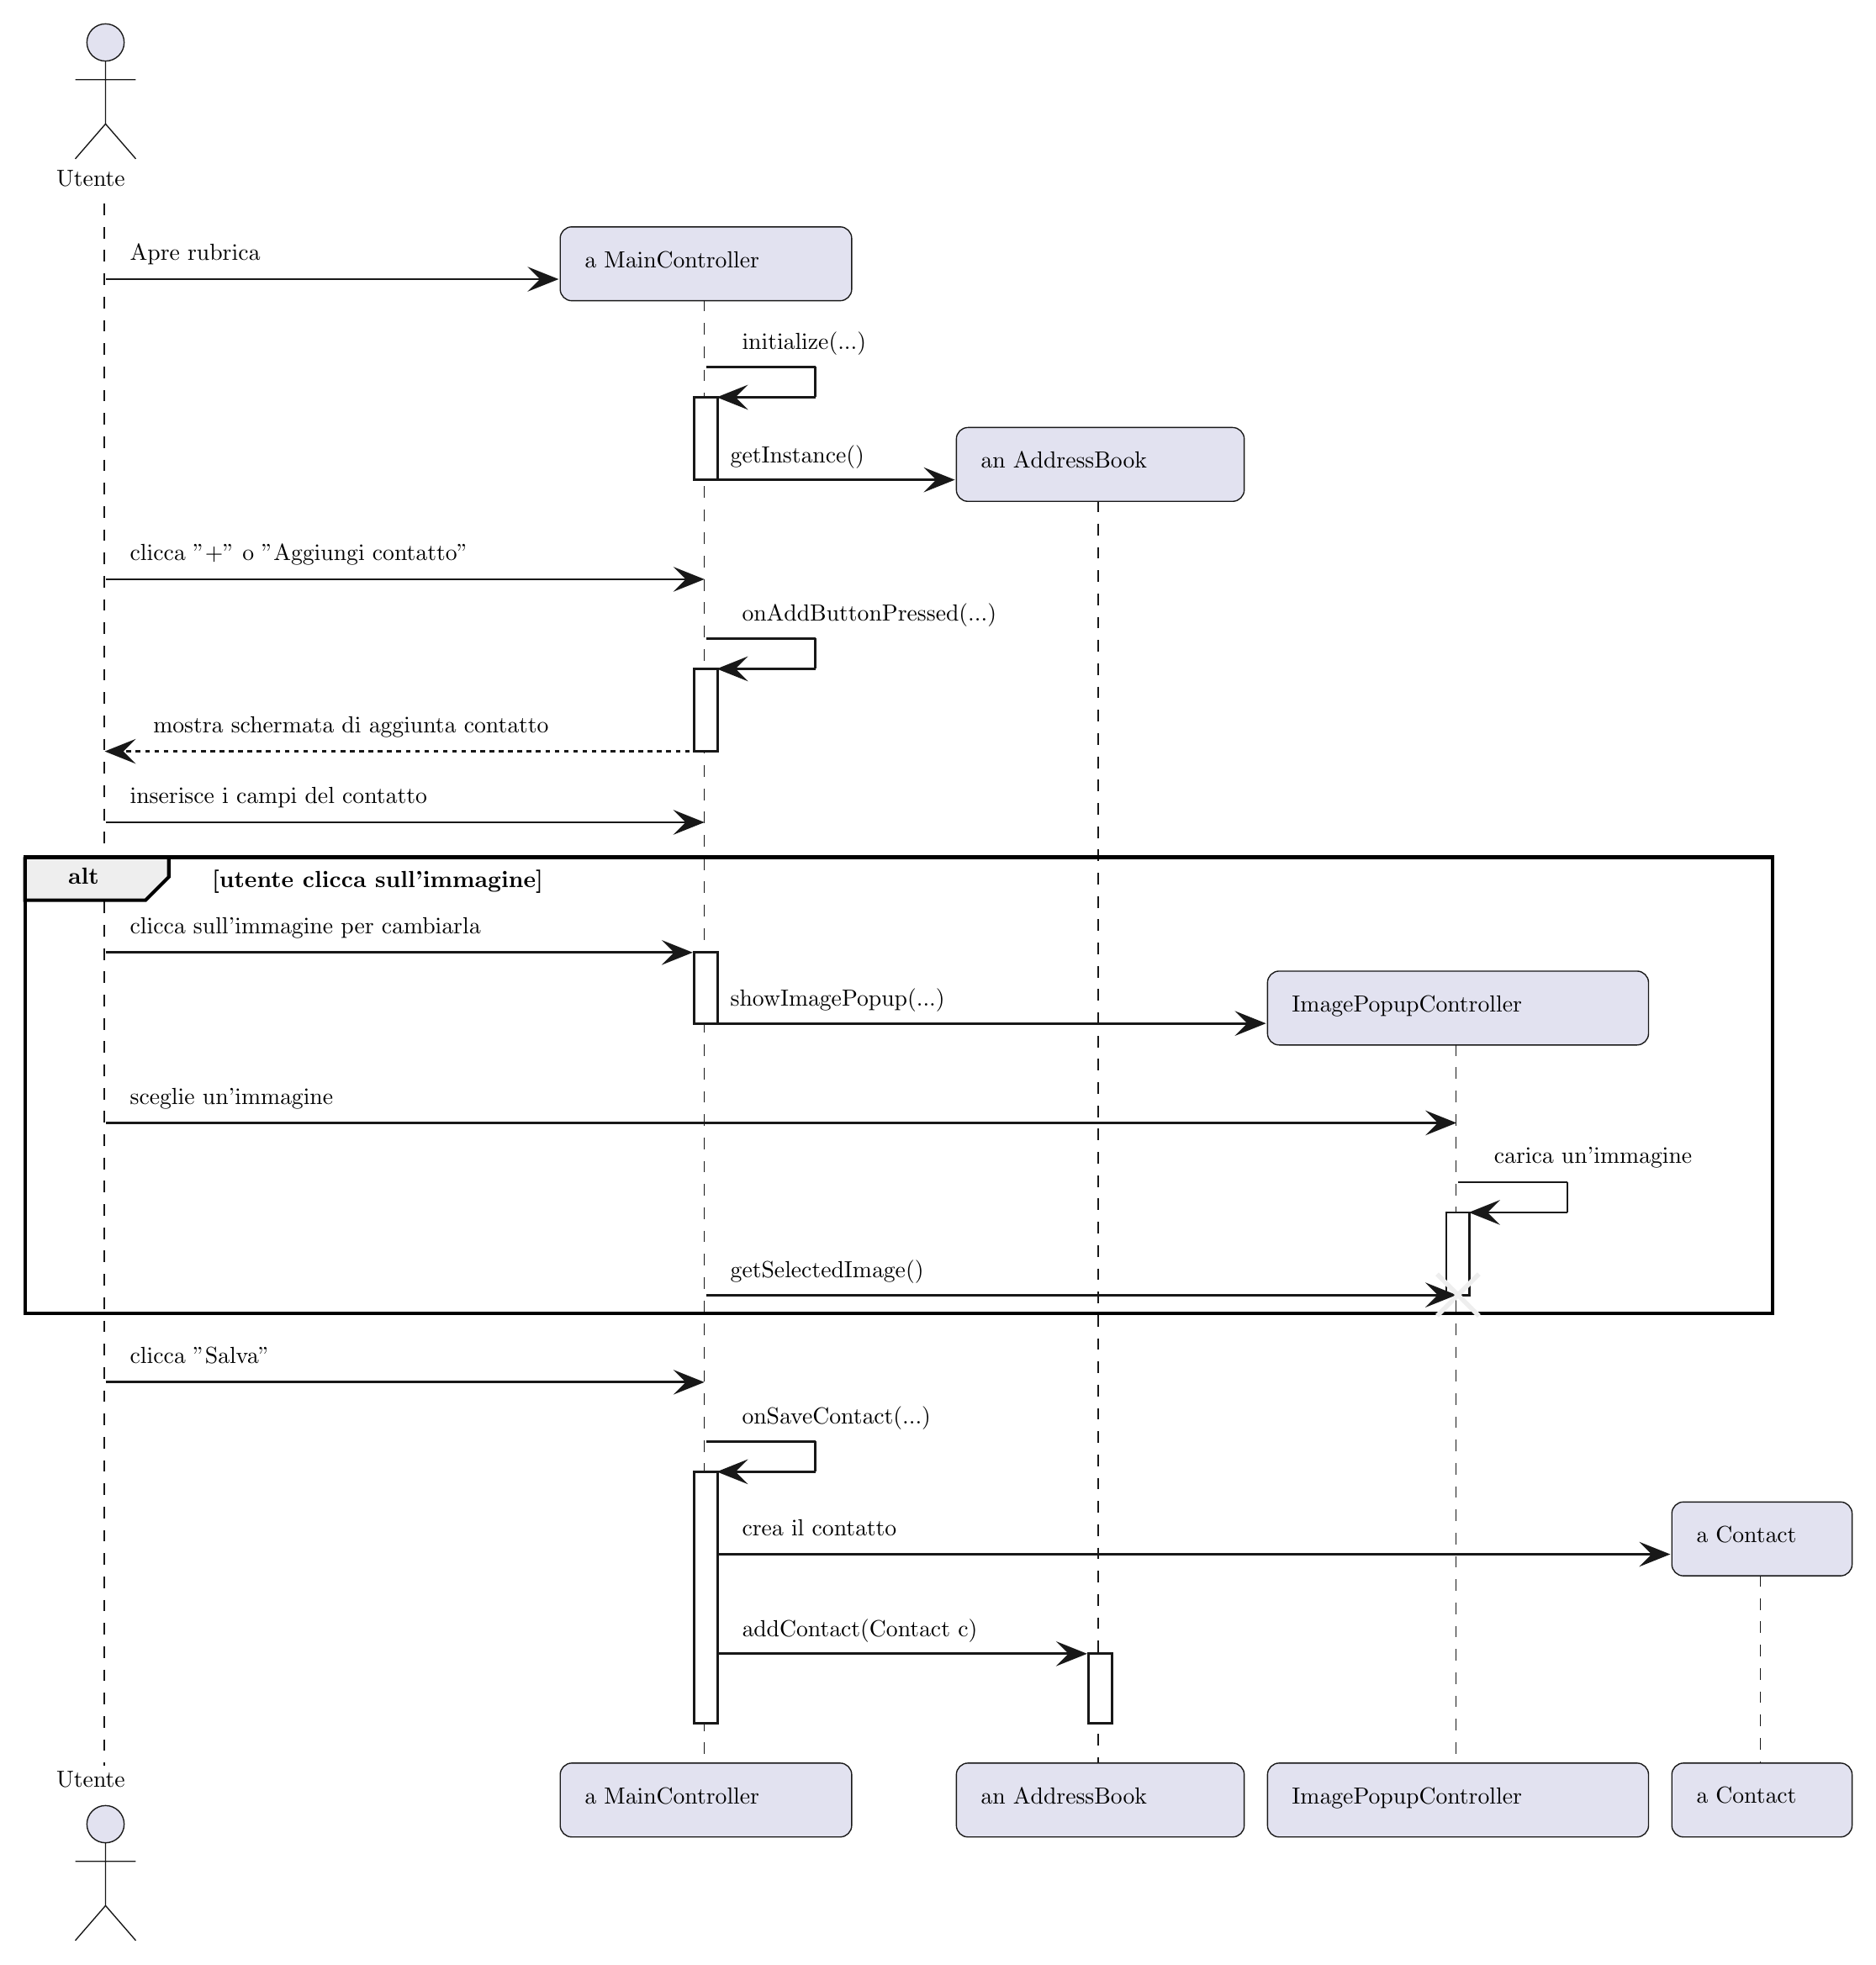
\begin{tikzpicture}[yscale=-1
,pstyle0/.style={color=plantucolor0001,fill=white,line width=1.0pt}
,pstyle1/.style={color=black,line width=1.5pt}
,pstyle2/.style={color=plantucolor0001,line width=0.5pt,dash pattern=on 5.0pt off 5.0pt}
,pstyle3/.style={color=plantucolor0001,fill=plantucolor0003,line width=0.5pt}
,pstyle4/.style={color=plantucolor0001,line width=0.5pt}
,pstyle5/.style={color=plantucolor0001,fill=plantucolor0001,line width=1.0pt}
,pstyle6/.style={color=plantucolor0001,line width=1.0pt}
,pstyle9/.style={color=plantucolor0005,line width=2.0pt}
]
\draw[pstyle0] (297.6157pt,165.9707pt) rectangle (307.6157pt,201.4492pt);
\draw[pstyle0] (297.6157pt,282.6738pt) rectangle (307.6157pt,318.1523pt);
\draw[pstyle0] (297.6157pt,404.5879pt) rectangle (307.6157pt,435.0664pt);
\draw[pstyle0] (297.6157pt,627.7266pt) rectangle (307.6157pt,735.9512pt);
\draw[pstyle0] (467.0763pt,705.9512pt) rectangle (477.0763pt,735.9512pt);
\draw[pstyle0] (620.8057pt,516.291pt) rectangle (630.8057pt,551.7695pt);
\draw[pstyle1] (10pt,363.6309pt) rectangle (761.0057pt,559.7695pt);
\draw[pstyle2] (44pt,82.7461pt) -- (44pt,753.9512pt);
\draw[pstyle2] (301.9816pt,124.1191pt) -- (301.9816pt,753.9512pt);
\draw[pstyle2] (471.2241pt,210.3438pt) -- (471.2241pt,753.9512pt);
\draw[pstyle2] (624.9285pt,443.9609pt) -- (624.9285pt,753.9512pt);
\draw[pstyle2] (755.6828pt,672.0996pt) -- (755.6828pt,753.9512pt);
\node at (20pt,65pt)[below right,color=black]{Utente};
\draw[pstyle3] (44.6pt,13.5pt) ellipse (8pt and 8pt);
\draw[pstyle4] (44.6pt,21.5pt) -- (44.6pt,48.5pt)(31.6pt,29.5pt) -- (57.6pt,29.5pt)(44.6pt,48.5pt) -- (31.6pt,63.5pt)(44.6pt,48.5pt) -- (57.6pt,63.5pt);
\node at (20pt,752.9512pt)[below right,color=black]{Utente};
\draw[pstyle3] (44.6pt,779.1973pt) ellipse (8pt and 8pt);
\draw[pstyle4] (44.6pt,787.1973pt) -- (44.6pt,814.1973pt)(31.6pt,795.1973pt) -- (57.6pt,795.1973pt)(44.6pt,814.1973pt) -- (31.6pt,829.1973pt)(44.6pt,814.1973pt) -- (57.6pt,829.1973pt);
\draw[pstyle3] (239.9816pt,757.9512pt) arc (180:270:5pt) -- (244.9816pt,752.9512pt) -- (360.2497pt,752.9512pt) arc (270:360:5pt) -- (365.2497pt,757.9512pt) -- (365.2497pt,779.6973pt) arc (0:90:5pt) -- (360.2497pt,784.6973pt) -- (244.9816pt,784.6973pt) arc (90:180:5pt) -- (239.9816pt,779.6973pt) -- cycle;
\node at (246.9816pt,759.9512pt)[below right,color=black]{a MainController};
\draw[pstyle3] (410.2241pt,757.9512pt) arc (180:270:5pt) -- (415.2241pt,752.9512pt) -- (528.9285pt,752.9512pt) arc (270:360:5pt) -- (533.9285pt,757.9512pt) -- (533.9285pt,779.6973pt) arc (0:90:5pt) -- (528.9285pt,784.6973pt) -- (415.2241pt,784.6973pt) arc (90:180:5pt) -- (410.2241pt,779.6973pt) -- cycle;
\node at (417.2241pt,759.9512pt)[below right,color=black]{an AddressBook};
\draw[pstyle3] (543.9285pt,757.9512pt) arc (180:270:5pt) -- (548.9285pt,752.9512pt) -- (702.6828pt,752.9512pt) arc (270:360:5pt) -- (707.6828pt,757.9512pt) -- (707.6828pt,779.6973pt) arc (0:90:5pt) -- (702.6828pt,784.6973pt) -- (548.9285pt,784.6973pt) arc (90:180:5pt) -- (543.9285pt,779.6973pt) -- cycle;
\node at (550.9285pt,759.9512pt)[below right,color=black]{ImagePopupController};
\draw[pstyle3] (717.6828pt,757.9512pt) arc (180:270:5pt) -- (722.6828pt,752.9512pt) -- (790.1495pt,752.9512pt) arc (270:360:5pt) -- (795.1495pt,757.9512pt) -- (795.1495pt,779.6973pt) arc (0:90:5pt) -- (790.1495pt,784.6973pt) -- (722.6828pt,784.6973pt) arc (90:180:5pt) -- (717.6828pt,779.6973pt) -- cycle;
\node at (724.6828pt,759.9512pt)[below right,color=black]{a Contact};
\draw[pstyle0] (297.6157pt,165.9707pt) rectangle (307.6157pt,201.4492pt);
\draw[pstyle0] (297.6157pt,282.6738pt) rectangle (307.6157pt,318.1523pt);
\draw[pstyle0] (297.6157pt,404.5879pt) rectangle (307.6157pt,435.0664pt);
\draw[pstyle0] (297.6157pt,627.7266pt) rectangle (307.6157pt,735.9512pt);
\draw[pstyle0] (467.0763pt,705.9512pt) rectangle (477.0763pt,735.9512pt);
\draw[pstyle0] (620.8057pt,516.291pt) rectangle (630.8057pt,551.7695pt);
\draw[pstyle5] (227.9816pt,111.2246pt) -- (237.9816pt,115.2246pt) -- (227.9816pt,119.2246pt) -- (231.9816pt,115.2246pt) -- cycle;
\draw[pstyle6] (44.6pt,115.2246pt) -- (233.9816pt,115.2246pt);
\node at (51.6pt,96.7461pt)[below right,color=black]{Apre rubrica};
\draw[pstyle3] (239.9816pt,97.7461pt) arc (180:270:5pt) -- (244.9816pt,92.7461pt) -- (360.2497pt,92.7461pt) arc (270:360:5pt) -- (365.2497pt,97.7461pt) -- (365.2497pt,119.4922pt) arc (0:90:5pt) -- (360.2497pt,124.4922pt) -- (244.9816pt,124.4922pt) arc (90:180:5pt) -- (239.9816pt,119.4922pt) -- cycle;
\node at (246.9816pt,99.7461pt)[below right,color=black]{a MainController};
\draw[pstyle6] (302.6157pt,152.9707pt) -- (349.6157pt,152.9707pt);
\draw[pstyle6] (349.6157pt,152.9707pt) -- (349.6157pt,165.9707pt);
\draw[pstyle6] (308.6157pt,165.9707pt) -- (349.6157pt,165.9707pt);
\draw[pstyle5] (318.6157pt,161.9707pt) -- (308.6157pt,165.9707pt) -- (318.6157pt,169.9707pt) -- (314.6157pt,165.9707pt) -- cycle;
\node at (314.6157pt,134.4922pt)[below right,color=black]{initialize(...)};
\draw[pstyle5] (398.2241pt,197.4492pt) -- (408.2241pt,201.4492pt) -- (398.2241pt,205.4492pt) -- (402.2241pt,201.4492pt) -- cycle;
\draw[pstyle6] (302.6157pt,201.4492pt) -- (404.2241pt,201.4492pt);
\node at (309.6157pt,182.9707pt)[below right,color=black]{getInstance()};
\draw[pstyle3] (410.2241pt,183.9707pt) arc (180:270:5pt) -- (415.2241pt,178.9707pt) -- (528.9285pt,178.9707pt) arc (270:360:5pt) -- (533.9285pt,183.9707pt) -- (533.9285pt,205.7168pt) arc (0:90:5pt) -- (528.9285pt,210.7168pt) -- (415.2241pt,210.7168pt) arc (90:180:5pt) -- (410.2241pt,205.7168pt) -- cycle;
\node at (417.2241pt,185.9707pt)[below right,color=black]{an AddressBook};
\draw[pstyle5] (290.6157pt,240.1953pt) -- (300.6157pt,244.1953pt) -- (290.6157pt,248.1953pt) -- (294.6157pt,244.1953pt) -- cycle;
\draw[pstyle6] (44.6pt,244.1953pt) -- (296.6157pt,244.1953pt);
\node at (51.6pt,225.7168pt)[below right,color=black]{clicca "+" o "Aggiungi contatto"};
\draw[pstyle6] (302.6157pt,269.6738pt) -- (349.6157pt,269.6738pt);
\draw[pstyle6] (349.6157pt,269.6738pt) -- (349.6157pt,282.6738pt);
\draw[pstyle6] (308.6157pt,282.6738pt) -- (349.6157pt,282.6738pt);
\draw[pstyle5] (318.6157pt,278.6738pt) -- (308.6157pt,282.6738pt) -- (318.6157pt,286.6738pt) -- (314.6157pt,282.6738pt) -- cycle;
\node at (314.6157pt,251.1953pt)[below right,color=black]{onAddButtonPressed(...)};
\draw[pstyle5] (55.6pt,314.1523pt) -- (45.6pt,318.1523pt) -- (55.6pt,322.1523pt) -- (51.6pt,318.1523pt) -- cycle;
\draw[color=plantucolor0001,line width=1.0pt,dash pattern=on 2.0pt off 2.0pt] (49.6pt,318.1523pt) -- (301.6157pt,318.1523pt);
\node at (61.6pt,299.6738pt)[below right,color=black]{mostra schermata di aggiunta contatto};
\draw[pstyle5] (290.6157pt,344.6309pt) -- (300.6157pt,348.6309pt) -- (290.6157pt,352.6309pt) -- (294.6157pt,348.6309pt) -- cycle;
\draw[pstyle6] (44.6pt,348.6309pt) -- (296.6157pt,348.6309pt);
\node at (51.6pt,330.1523pt)[below right,color=black]{inserisce i campi del contatto};
\draw[color=black,fill=plantucolor0004,line width=1.5pt] (10pt,363.6309pt) -- (71.8pt,363.6309pt) -- (71.8pt,372.1094pt) -- (61.8pt,382.1094pt) -- (10pt,382.1094pt) -- (10pt,363.6309pt);
\draw[pstyle1] (10pt,363.6309pt) rectangle (761.0057pt,559.7695pt);
\node at (25pt,364.6309pt)[below right,color=black]{\textbf{alt}};
\node at (86.8pt,365.6309pt)[below right,color=black]{\textbf{[utente clicca sull'immagine]}};
\draw[pstyle5] (285.6157pt,400.5879pt) -- (295.6157pt,404.5879pt) -- (285.6157pt,408.5879pt) -- (289.6157pt,404.5879pt) -- cycle;
\draw[pstyle6] (44.6pt,404.5879pt) -- (291.6157pt,404.5879pt);
\node at (51.6pt,386.1094pt)[below right,color=black]{clicca sull'immagine per cambiarla};
\draw[pstyle5] (531.9285pt,431.0664pt) -- (541.9285pt,435.0664pt) -- (531.9285pt,439.0664pt) -- (535.9285pt,435.0664pt) -- cycle;
\draw[pstyle6] (302.6157pt,435.0664pt) -- (537.9285pt,435.0664pt);
\node at (309.6157pt,416.5879pt)[below right,color=black]{showImagePopup(...)};
\draw[pstyle3] (543.9285pt,417.5879pt) arc (180:270:5pt) -- (548.9285pt,412.5879pt) -- (702.6828pt,412.5879pt) arc (270:360:5pt) -- (707.6828pt,417.5879pt) -- (707.6828pt,439.334pt) arc (0:90:5pt) -- (702.6828pt,444.334pt) -- (548.9285pt,444.334pt) arc (90:180:5pt) -- (543.9285pt,439.334pt) -- cycle;
\node at (550.9285pt,419.5879pt)[below right,color=black]{ImagePopupController};
\draw[pstyle5] (613.8057pt,473.8125pt) -- (623.8057pt,477.8125pt) -- (613.8057pt,481.8125pt) -- (617.8057pt,477.8125pt) -- cycle;
\draw[pstyle6] (44.6pt,477.8125pt) -- (619.8057pt,477.8125pt);
\node at (51.6pt,459.334pt)[below right,color=black]{sceglie un'immagine};
\draw[pstyle6] (625.8057pt,503.291pt) -- (672.8057pt,503.291pt);
\draw[pstyle6] (672.8057pt,503.291pt) -- (672.8057pt,516.291pt);
\draw[pstyle6] (631.8057pt,516.291pt) -- (672.8057pt,516.291pt);
\draw[pstyle5] (641.8057pt,512.291pt) -- (631.8057pt,516.291pt) -- (641.8057pt,520.291pt) -- (637.8057pt,516.291pt) -- cycle;
\node at (637.8057pt,484.8125pt)[below right,color=black]{carica un'immagine};
\draw[pstyle5] (613.8057pt,547.7695pt) -- (623.8057pt,551.7695pt) -- (613.8057pt,555.7695pt) -- (617.8057pt,551.7695pt) -- cycle;
\draw[pstyle6] (302.6157pt,551.7695pt) -- (619.8057pt,551.7695pt);
\node at (309.6157pt,533.291pt)[below right,color=black]{getSelectedImage()};
\draw[pstyle9] (616.8057pt,542.7695pt) -- (634.8057pt,560.7695pt);
\draw[pstyle9] (616.8057pt,560.7695pt) -- (634.8057pt,542.7695pt);
\draw[pstyle5] (290.6157pt,585.248pt) -- (300.6157pt,589.248pt) -- (290.6157pt,593.248pt) -- (294.6157pt,589.248pt) -- cycle;
\draw[pstyle6] (44.6pt,589.248pt) -- (296.6157pt,589.248pt);
\node at (51.6pt,570.7695pt)[below right,color=black]{clicca "Salva"};
\draw[pstyle6] (302.6157pt,614.7266pt) -- (349.6157pt,614.7266pt);
\draw[pstyle6] (349.6157pt,614.7266pt) -- (349.6157pt,627.7266pt);
\draw[pstyle6] (308.6157pt,627.7266pt) -- (349.6157pt,627.7266pt);
\draw[pstyle5] (318.6157pt,623.7266pt) -- (308.6157pt,627.7266pt) -- (318.6157pt,631.7266pt) -- (314.6157pt,627.7266pt) -- cycle;
\node at (314.6157pt,596.248pt)[below right,color=black]{onSaveContact(...)};
\draw[pstyle5] (705.6828pt,659.2051pt) -- (715.6828pt,663.2051pt) -- (705.6828pt,667.2051pt) -- (709.6828pt,663.2051pt) -- cycle;
\draw[pstyle6] (307.6157pt,663.2051pt) -- (711.6828pt,663.2051pt);
\node at (314.6157pt,644.7266pt)[below right,color=black]{crea il contatto};
\draw[pstyle3] (717.6828pt,645.7266pt) arc (180:270:5pt) -- (722.6828pt,640.7266pt) -- (790.1495pt,640.7266pt) arc (270:360:5pt) -- (795.1495pt,645.7266pt) -- (795.1495pt,667.4727pt) arc (0:90:5pt) -- (790.1495pt,672.4727pt) -- (722.6828pt,672.4727pt) arc (90:180:5pt) -- (717.6828pt,667.4727pt) -- cycle;
\node at (724.6828pt,647.7266pt)[below right,color=black]{a Contact};
\draw[pstyle5] (455.0763pt,701.9512pt) -- (465.0763pt,705.9512pt) -- (455.0763pt,709.9512pt) -- (459.0763pt,705.9512pt) -- cycle;
\draw[pstyle6] (307.6157pt,705.9512pt) -- (461.0763pt,705.9512pt);
\node at (314.6157pt,687.4727pt)[below right,color=black]{addContact(Contact c)};
\end{tikzpicture}
}
\end{adjustbox}

\begin{figure}[h]
\caption{Diagramma sequenza C1 - Aggiungere Contatto}
\label{fig:Diagramma sequenza C1 - Aggiungere Contatto}
\end{figure}

\newpage
\subsubsection{C2 C3 - Eliminare Modificare Contatto}
Il seguente diagramma di sequenza illustra l'esecuzione di entrambi i casi d'uso C2 e C3, tramite la sintassi \texttt{loop}, \texttt{break} e \texttt{alt}:
% generated by Plantuml 1.2024.3       
\definecolor{plantucolor0000}{RGB}{255,255,255}
\definecolor{plantucolor0001}{RGB}{24,24,24}
\definecolor{plantucolor0002}{RGB}{0,0,0}
\definecolor{plantucolor0003}{RGB}{226,226,240}
\definecolor{plantucolor0004}{RGB}{238,238,238}

\begin{adjustbox}{width=.84\paperwidth, center}
	\resizebox{\textwidth}{!}{
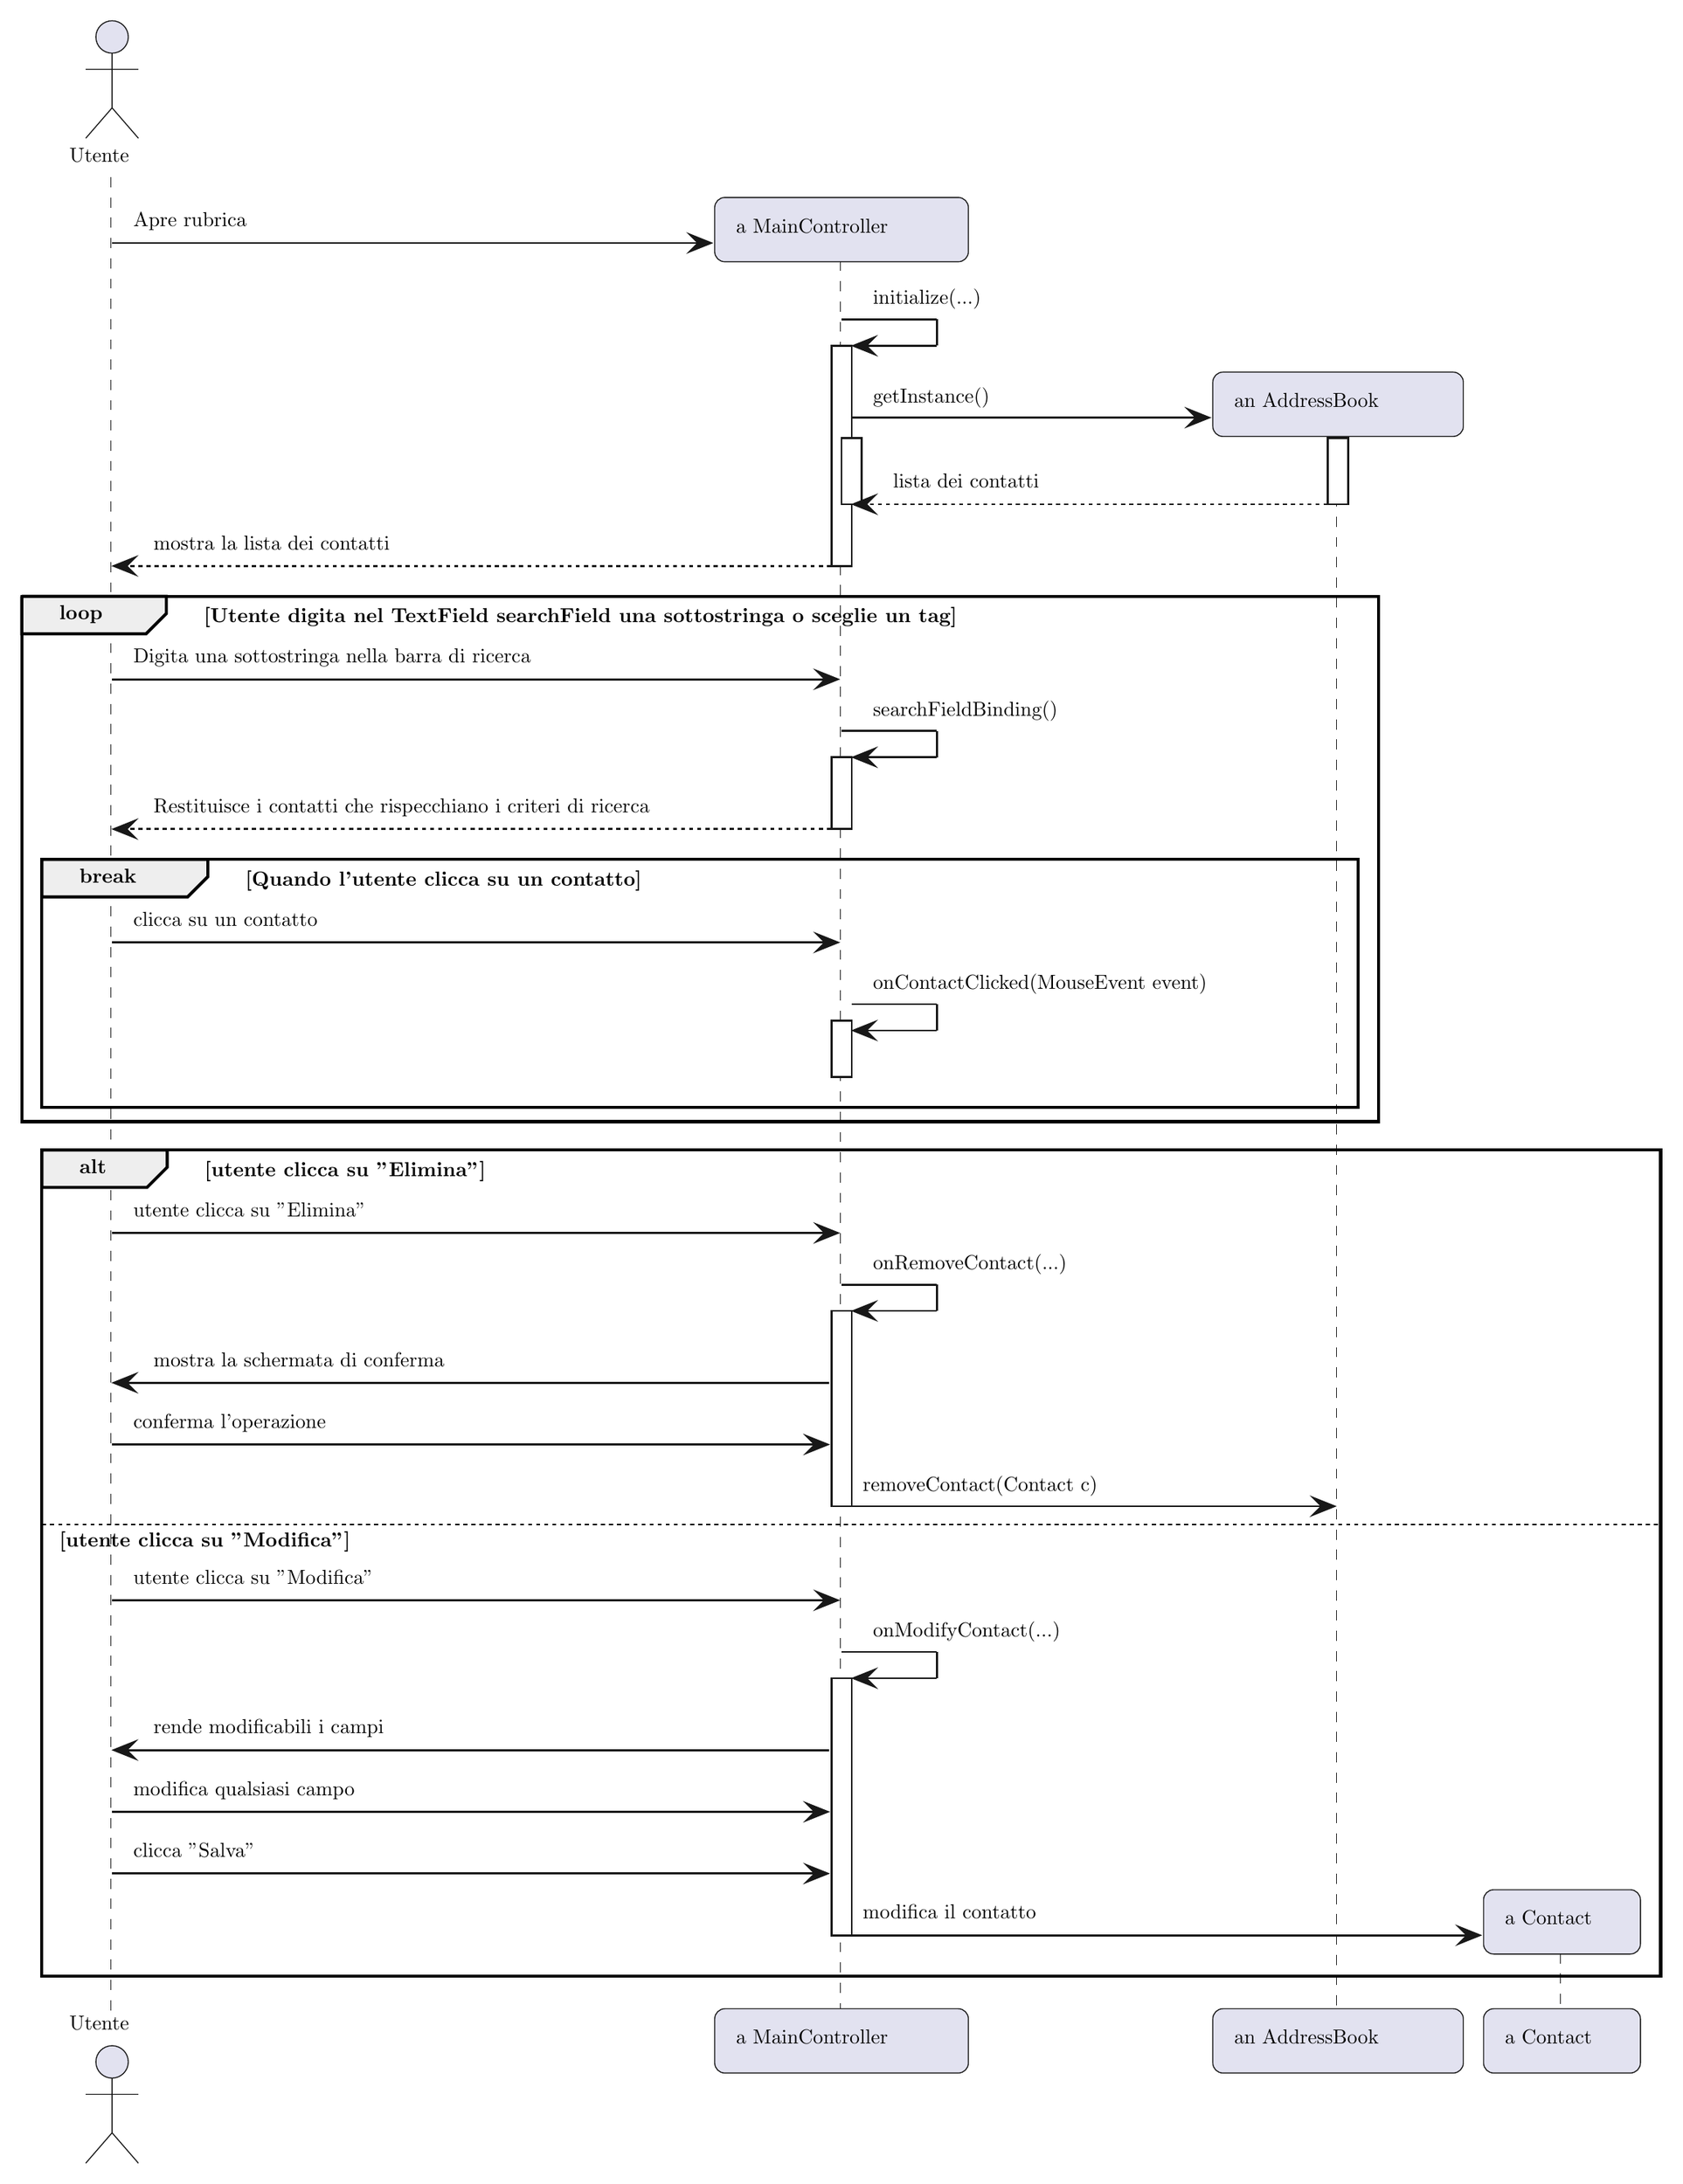
\begin{tikzpicture}[yscale=-1
,pstyle0/.style={color=plantucolor0001,fill=white,line width=1.0pt}
,pstyle1/.style={color=black,line width=1.5pt}
,pstyle2/.style={color=plantucolor0001,line width=0.5pt,dash pattern=on 5.0pt off 5.0pt}
,pstyle3/.style={color=plantucolor0001,fill=plantucolor0003,line width=0.5pt}
,pstyle4/.style={color=plantucolor0001,line width=0.5pt}
,pstyle5/.style={color=plantucolor0001,fill=plantucolor0001,line width=1.0pt}
,pstyle6/.style={color=plantucolor0001,line width=1.0pt}
,pstyle7/.style={color=plantucolor0001,line width=1.0pt,dash pattern=on 2.0pt off 2.0pt}
,pstyle8/.style={color=black,fill=plantucolor0004,line width=1.5pt}
]
\draw[pstyle0] (409.8219pt,165.9707pt) rectangle (419.8219pt,274.6738pt);
\draw[pstyle0] (414.8219pt,211.4492pt) rectangle (424.8219pt,244.1953pt);
\draw[pstyle0] (409.8219pt,369.1094pt) rectangle (419.8219pt,404.5879pt);
\draw[pstyle0] (409.8219pt,499.0234pt) rectangle (419.8219pt,527.0234pt);
\draw[pstyle0] (409.8219pt,642.459pt) rectangle (419.8219pt,738.8945pt);
\draw[pstyle0] (409.8219pt,823.7949pt) rectangle (419.8219pt,950.709pt);
\draw[pstyle0] (655.0081pt,211.4492pt) rectangle (665.0081pt,244.1953pt);
\draw[pstyle1] (10pt,289.6738pt) rectangle (680.0081pt,549.0234pt);
\draw[pstyle1] (20pt,419.5879pt) rectangle (670.0081pt,542.0234pt);
\draw[pstyle1] (20pt,563.0234pt) rectangle (819.327pt,970.9766pt);
\draw[pstyle2] (54pt,82.7461pt) -- (54pt,987.9766pt);
\draw[pstyle2] (414.1879pt,124.1191pt) -- (414.1879pt,987.9766pt);
\draw[pstyle2] (659.156pt,210.3438pt) -- (659.156pt,987.9766pt);
\draw[pstyle2] (769.8603pt,959.6035pt) -- (769.8603pt,987.9766pt);
\node at (30pt,65pt)[below right,color=black]{Utente};
\draw[pstyle3] (54.6pt,13.5pt) ellipse (8pt and 8pt);
\draw[pstyle4] (54.6pt,21.5pt) -- (54.6pt,48.5pt)(41.6pt,29.5pt) -- (67.6pt,29.5pt)(54.6pt,48.5pt) -- (41.6pt,63.5pt)(54.6pt,48.5pt) -- (67.6pt,63.5pt);
\node at (30pt,986.9766pt)[below right,color=black]{Utente};
\draw[pstyle3] (54.6pt,1013.2227pt) ellipse (8pt and 8pt);
\draw[pstyle4] (54.6pt,1021.2227pt) -- (54.6pt,1048.2227pt)(41.6pt,1029.2227pt) -- (67.6pt,1029.2227pt)(54.6pt,1048.2227pt) -- (41.6pt,1063.2227pt)(54.6pt,1048.2227pt) -- (67.6pt,1063.2227pt);
\draw[pstyle3] (352.1879pt,991.9766pt) arc (180:270:5pt) -- (357.1879pt,986.9766pt) -- (472.456pt,986.9766pt) arc (270:360:5pt) -- (477.456pt,991.9766pt) -- (477.456pt,1013.7227pt) arc (0:90:5pt) -- (472.456pt,1018.7227pt) -- (357.1879pt,1018.7227pt) arc (90:180:5pt) -- (352.1879pt,1013.7227pt) -- cycle;
\node at (359.1879pt,993.9766pt)[below right,color=black]{a MainController};
\draw[pstyle3] (598.156pt,991.9766pt) arc (180:270:5pt) -- (603.156pt,986.9766pt) -- (716.8603pt,986.9766pt) arc (270:360:5pt) -- (721.8603pt,991.9766pt) -- (721.8603pt,1013.7227pt) arc (0:90:5pt) -- (716.8603pt,1018.7227pt) -- (603.156pt,1018.7227pt) arc (90:180:5pt) -- (598.156pt,1013.7227pt) -- cycle;
\node at (605.156pt,993.9766pt)[below right,color=black]{an AddressBook};
\draw[pstyle3] (731.8603pt,991.9766pt) arc (180:270:5pt) -- (736.8603pt,986.9766pt) -- (804.327pt,986.9766pt) arc (270:360:5pt) -- (809.327pt,991.9766pt) -- (809.327pt,1013.7227pt) arc (0:90:5pt) -- (804.327pt,1018.7227pt) -- (736.8603pt,1018.7227pt) arc (90:180:5pt) -- (731.8603pt,1013.7227pt) -- cycle;
\node at (738.8603pt,993.9766pt)[below right,color=black]{a Contact};
\draw[pstyle0] (409.8219pt,165.9707pt) rectangle (419.8219pt,274.6738pt);
\draw[pstyle0] (414.8219pt,211.4492pt) rectangle (424.8219pt,244.1953pt);
\draw[pstyle0] (409.8219pt,369.1094pt) rectangle (419.8219pt,404.5879pt);
\draw[pstyle0] (409.8219pt,499.0234pt) rectangle (419.8219pt,527.0234pt);
\draw[pstyle0] (409.8219pt,642.459pt) rectangle (419.8219pt,738.8945pt);
\draw[pstyle0] (409.8219pt,823.7949pt) rectangle (419.8219pt,950.709pt);
\draw[pstyle0] (655.0081pt,211.4492pt) rectangle (665.0081pt,244.1953pt);
\draw[pstyle5] (340.1879pt,111.2246pt) -- (350.1879pt,115.2246pt) -- (340.1879pt,119.2246pt) -- (344.1879pt,115.2246pt) -- cycle;
\draw[pstyle6] (54.6pt,115.2246pt) -- (346.1879pt,115.2246pt);
\node at (61.6pt,96.7461pt)[below right,color=black]{Apre rubrica};
\draw[pstyle3] (352.1879pt,97.7461pt) arc (180:270:5pt) -- (357.1879pt,92.7461pt) -- (472.456pt,92.7461pt) arc (270:360:5pt) -- (477.456pt,97.7461pt) -- (477.456pt,119.4922pt) arc (0:90:5pt) -- (472.456pt,124.4922pt) -- (357.1879pt,124.4922pt) arc (90:180:5pt) -- (352.1879pt,119.4922pt) -- cycle;
\node at (359.1879pt,99.7461pt)[below right,color=black]{a MainController};
\draw[pstyle6] (414.8219pt,152.9707pt) -- (461.8219pt,152.9707pt);
\draw[pstyle6] (461.8219pt,152.9707pt) -- (461.8219pt,165.9707pt);
\draw[pstyle6] (420.8219pt,165.9707pt) -- (461.8219pt,165.9707pt);
\draw[pstyle5] (430.8219pt,161.9707pt) -- (420.8219pt,165.9707pt) -- (430.8219pt,169.9707pt) -- (426.8219pt,165.9707pt) -- cycle;
\node at (426.8219pt,134.4922pt)[below right,color=black]{initialize(...)};
\draw[pstyle5] (586.156pt,197.4492pt) -- (596.156pt,201.4492pt) -- (586.156pt,205.4492pt) -- (590.156pt,201.4492pt) -- cycle;
\draw[pstyle6] (419.8219pt,201.4492pt) -- (592.156pt,201.4492pt);
\node at (426.8219pt,182.9707pt)[below right,color=black]{getInstance()};
\draw[pstyle3] (598.156pt,183.9707pt) arc (180:270:5pt) -- (603.156pt,178.9707pt) -- (716.8603pt,178.9707pt) arc (270:360:5pt) -- (721.8603pt,183.9707pt) -- (721.8603pt,205.7168pt) arc (0:90:5pt) -- (716.8603pt,210.7168pt) -- (603.156pt,210.7168pt) arc (90:180:5pt) -- (598.156pt,205.7168pt) -- cycle;
\node at (605.156pt,185.9707pt)[below right,color=black]{an AddressBook};
\draw[pstyle5] (430.8219pt,240.1953pt) -- (420.8219pt,244.1953pt) -- (430.8219pt,248.1953pt) -- (426.8219pt,244.1953pt) -- cycle;
\draw[pstyle7] (424.8219pt,244.1953pt) -- (659.0081pt,244.1953pt);
\node at (436.8219pt,225.7168pt)[below right,color=black]{lista dei contatti};
\draw[pstyle5] (65.6pt,270.6738pt) -- (55.6pt,274.6738pt) -- (65.6pt,278.6738pt) -- (61.6pt,274.6738pt) -- cycle;
\draw[pstyle7] (59.6pt,274.6738pt) -- (413.8219pt,274.6738pt);
\node at (71.6pt,256.1953pt)[below right,color=black]{mostra la lista dei contatti};
\draw[pstyle8] (10pt,289.6738pt) -- (81.4pt,289.6738pt) -- (81.4pt,298.1523pt) -- (71.4pt,308.1523pt) -- (10pt,308.1523pt) -- (10pt,289.6738pt);
\draw[pstyle1] (10pt,289.6738pt) rectangle (680.0081pt,549.0234pt);
\node at (25pt,290.6738pt)[below right,color=black]{\textbf{loop}};
\node at (96.4pt,291.6738pt)[below right,color=black]{\textbf{[Utente digita nel TextField searchField una sottostringa o sceglie un tag]}};
\draw[pstyle5] (402.8219pt,326.6309pt) -- (412.8219pt,330.6309pt) -- (402.8219pt,334.6309pt) -- (406.8219pt,330.6309pt) -- cycle;
\draw[pstyle6] (54.6pt,330.6309pt) -- (408.8219pt,330.6309pt);
\node at (61.6pt,312.1523pt)[below right,color=black]{Digita una sottostringa nella barra di ricerca};
\draw[pstyle6] (414.8219pt,356.1094pt) -- (461.8219pt,356.1094pt);
\draw[pstyle6] (461.8219pt,356.1094pt) -- (461.8219pt,369.1094pt);
\draw[pstyle6] (420.8219pt,369.1094pt) -- (461.8219pt,369.1094pt);
\draw[pstyle5] (430.8219pt,365.1094pt) -- (420.8219pt,369.1094pt) -- (430.8219pt,373.1094pt) -- (426.8219pt,369.1094pt) -- cycle;
\node at (426.8219pt,337.6309pt)[below right,color=black]{searchFieldBinding()};
\draw[pstyle5] (65.6pt,400.5879pt) -- (55.6pt,404.5879pt) -- (65.6pt,408.5879pt) -- (61.6pt,404.5879pt) -- cycle;
\draw[pstyle7] (59.6pt,404.5879pt) -- (413.8219pt,404.5879pt);
\node at (71.6pt,386.1094pt)[below right,color=black]{Restituisce i contatti che rispecchiano i criteri di ricerca};
\draw[pstyle8] (20pt,419.5879pt) -- (101.9pt,419.5879pt) -- (101.9pt,428.0664pt) -- (91.9pt,438.0664pt) -- (20pt,438.0664pt) -- (20pt,419.5879pt);
\draw[pstyle1] (20pt,419.5879pt) rectangle (670.0081pt,542.0234pt);
\node at (35pt,420.5879pt)[below right,color=black]{\textbf{break}};
\node at (116.9pt,421.5879pt)[below right,color=black]{\textbf{[Quando l'utente clicca su un contatto]}};
\draw[pstyle5] (402.8219pt,456.5449pt) -- (412.8219pt,460.5449pt) -- (402.8219pt,464.5449pt) -- (406.8219pt,460.5449pt) -- cycle;
\draw[pstyle6] (54.6pt,460.5449pt) -- (408.8219pt,460.5449pt);
\node at (61.6pt,442.0664pt)[below right,color=black]{clicca su un contatto};
\draw[pstyle6] (419.8219pt,491.0234pt) -- (461.8219pt,491.0234pt);
\draw[pstyle6] (461.8219pt,491.0234pt) -- (461.8219pt,504.0234pt);
\draw[pstyle6] (420.8219pt,504.0234pt) -- (461.8219pt,504.0234pt);
\draw[pstyle5] (430.8219pt,500.0234pt) -- (420.8219pt,504.0234pt) -- (430.8219pt,508.0234pt) -- (426.8219pt,504.0234pt) -- cycle;
\node at (426.8219pt,472.5449pt)[below right,color=black]{onContactClicked(MouseEvent event)};
\draw[pstyle8] (20pt,563.0234pt) -- (81.8pt,563.0234pt) -- (81.8pt,571.502pt) -- (71.8pt,581.502pt) -- (20pt,581.502pt) -- (20pt,563.0234pt);
\draw[pstyle1] (20pt,563.0234pt) rectangle (819.327pt,970.9766pt);
\node at (35pt,564.0234pt)[below right,color=black]{\textbf{alt}};
\node at (96.8pt,565.0234pt)[below right,color=black]{\textbf{[utente clicca su "Elimina"]}};
\draw[pstyle5] (402.8219pt,599.9805pt) -- (412.8219pt,603.9805pt) -- (402.8219pt,607.9805pt) -- (406.8219pt,603.9805pt) -- cycle;
\draw[pstyle6] (54.6pt,603.9805pt) -- (408.8219pt,603.9805pt);
\node at (61.6pt,585.502pt)[below right,color=black]{utente clicca su "Elimina"};
\draw[pstyle6] (414.8219pt,629.459pt) -- (461.8219pt,629.459pt);
\draw[pstyle6] (461.8219pt,629.459pt) -- (461.8219pt,642.459pt);
\draw[pstyle6] (420.8219pt,642.459pt) -- (461.8219pt,642.459pt);
\draw[pstyle5] (430.8219pt,638.459pt) -- (420.8219pt,642.459pt) -- (430.8219pt,646.459pt) -- (426.8219pt,642.459pt) -- cycle;
\node at (426.8219pt,610.9805pt)[below right,color=black]{onRemoveContact(...)};
\draw[pstyle5] (65.6pt,673.9375pt) -- (55.6pt,677.9375pt) -- (65.6pt,681.9375pt) -- (61.6pt,677.9375pt) -- cycle;
\draw[pstyle6] (59.6pt,677.9375pt) -- (408.8219pt,677.9375pt);
\node at (71.6pt,659.459pt)[below right,color=black]{mostra la schermata di conferma};
\draw[pstyle5] (397.8219pt,704.416pt) -- (407.8219pt,708.416pt) -- (397.8219pt,712.416pt) -- (401.8219pt,708.416pt) -- cycle;
\draw[pstyle6] (54.6pt,708.416pt) -- (403.8219pt,708.416pt);
\node at (61.6pt,689.9375pt)[below right,color=black]{conferma l'operazione};
\draw[pstyle5] (648.0081pt,734.8945pt) -- (658.0081pt,738.8945pt) -- (648.0081pt,742.8945pt) -- (652.0081pt,738.8945pt) -- cycle;
\draw[pstyle6] (414.8219pt,738.8945pt) -- (654.0081pt,738.8945pt);
\node at (421.8219pt,720.416pt)[below right,color=black]{removeContact(Contact c)};
\draw[color=black,line width=1.0pt,dash pattern=on 2.0pt off 2.0pt] (20pt,747.8945pt) -- (819.327pt,747.8945pt);
\node at (25pt,747.8945pt)[below right,color=black]{\textbf{[utente clicca su "Modifica"]}};
\draw[pstyle5] (402.8219pt,781.3164pt) -- (412.8219pt,785.3164pt) -- (402.8219pt,789.3164pt) -- (406.8219pt,785.3164pt) -- cycle;
\draw[pstyle6] (54.6pt,785.3164pt) -- (408.8219pt,785.3164pt);
\node at (61.6pt,766.8379pt)[below right,color=black]{utente clicca su "Modifica"};
\draw[pstyle6] (414.8219pt,810.7949pt) -- (461.8219pt,810.7949pt);
\draw[pstyle6] (461.8219pt,810.7949pt) -- (461.8219pt,823.7949pt);
\draw[pstyle6] (420.8219pt,823.7949pt) -- (461.8219pt,823.7949pt);
\draw[pstyle5] (430.8219pt,819.7949pt) -- (420.8219pt,823.7949pt) -- (430.8219pt,827.7949pt) -- (426.8219pt,823.7949pt) -- cycle;
\node at (426.8219pt,792.3164pt)[below right,color=black]{onModifyContact(...)};
\draw[pstyle5] (65.6pt,855.2734pt) -- (55.6pt,859.2734pt) -- (65.6pt,863.2734pt) -- (61.6pt,859.2734pt) -- cycle;
\draw[pstyle6] (59.6pt,859.2734pt) -- (408.8219pt,859.2734pt);
\node at (71.6pt,840.7949pt)[below right,color=black]{rende modificabili i campi};
\draw[pstyle5] (397.8219pt,885.752pt) -- (407.8219pt,889.752pt) -- (397.8219pt,893.752pt) -- (401.8219pt,889.752pt) -- cycle;
\draw[pstyle6] (54.6pt,889.752pt) -- (403.8219pt,889.752pt);
\node at (61.6pt,871.2734pt)[below right,color=black]{modifica qualsiasi campo};
\draw[pstyle5] (397.8219pt,916.2305pt) -- (407.8219pt,920.2305pt) -- (397.8219pt,924.2305pt) -- (401.8219pt,920.2305pt) -- cycle;
\draw[pstyle6] (54.6pt,920.2305pt) -- (403.8219pt,920.2305pt);
\node at (61.6pt,901.752pt)[below right,color=black]{clicca "Salva"};
\draw[pstyle5] (719.8603pt,946.709pt) -- (729.8603pt,950.709pt) -- (719.8603pt,954.709pt) -- (723.8603pt,950.709pt) -- cycle;
\draw[pstyle6] (414.8219pt,950.709pt) -- (725.8603pt,950.709pt);
\node at (421.8219pt,932.2305pt)[below right,color=black]{modifica il contatto};
\draw[pstyle3] (731.8603pt,933.2305pt) arc (180:270:5pt) -- (736.8603pt,928.2305pt) -- (804.327pt,928.2305pt) arc (270:360:5pt) -- (809.327pt,933.2305pt) -- (809.327pt,954.9766pt) arc (0:90:5pt) -- (804.327pt,959.9766pt) -- (736.8603pt,959.9766pt) arc (90:180:5pt) -- (731.8603pt,954.9766pt) -- cycle;
\node at (738.8603pt,935.2305pt)[below right,color=black]{a Contact};
\end{tikzpicture}
}
\end{adjustbox}
\begin{figure}[h]
\caption{Diagramma sequenza C2 C3 - Eliminare Modificare Contatto}
\label{fig:Diagramma sequenza C2 C3 - Eliminare Modificare Contatto}
\end{figure}

\newpage
\subsubsection{C5 - Importare rubrica}
Il seguente diagramma di sequenza illustra l'esecuzione del caso d'uso C5:
% generated by Plantuml 1.2024.3       
\definecolor{plantucolor0000}{RGB}{255,255,255}
\definecolor{plantucolor0001}{RGB}{24,24,24}
\definecolor{plantucolor0002}{RGB}{0,0,0}
\definecolor{plantucolor0003}{RGB}{226,226,240}
\definecolor{plantucolor0004}{RGB}{238,238,238}
\definecolor{plantucolor0005}{RGB}{168,0,54}

\begin{adjustbox}{width=.9\paperwidth, center}
	\resizebox{\textwidth}{!}{
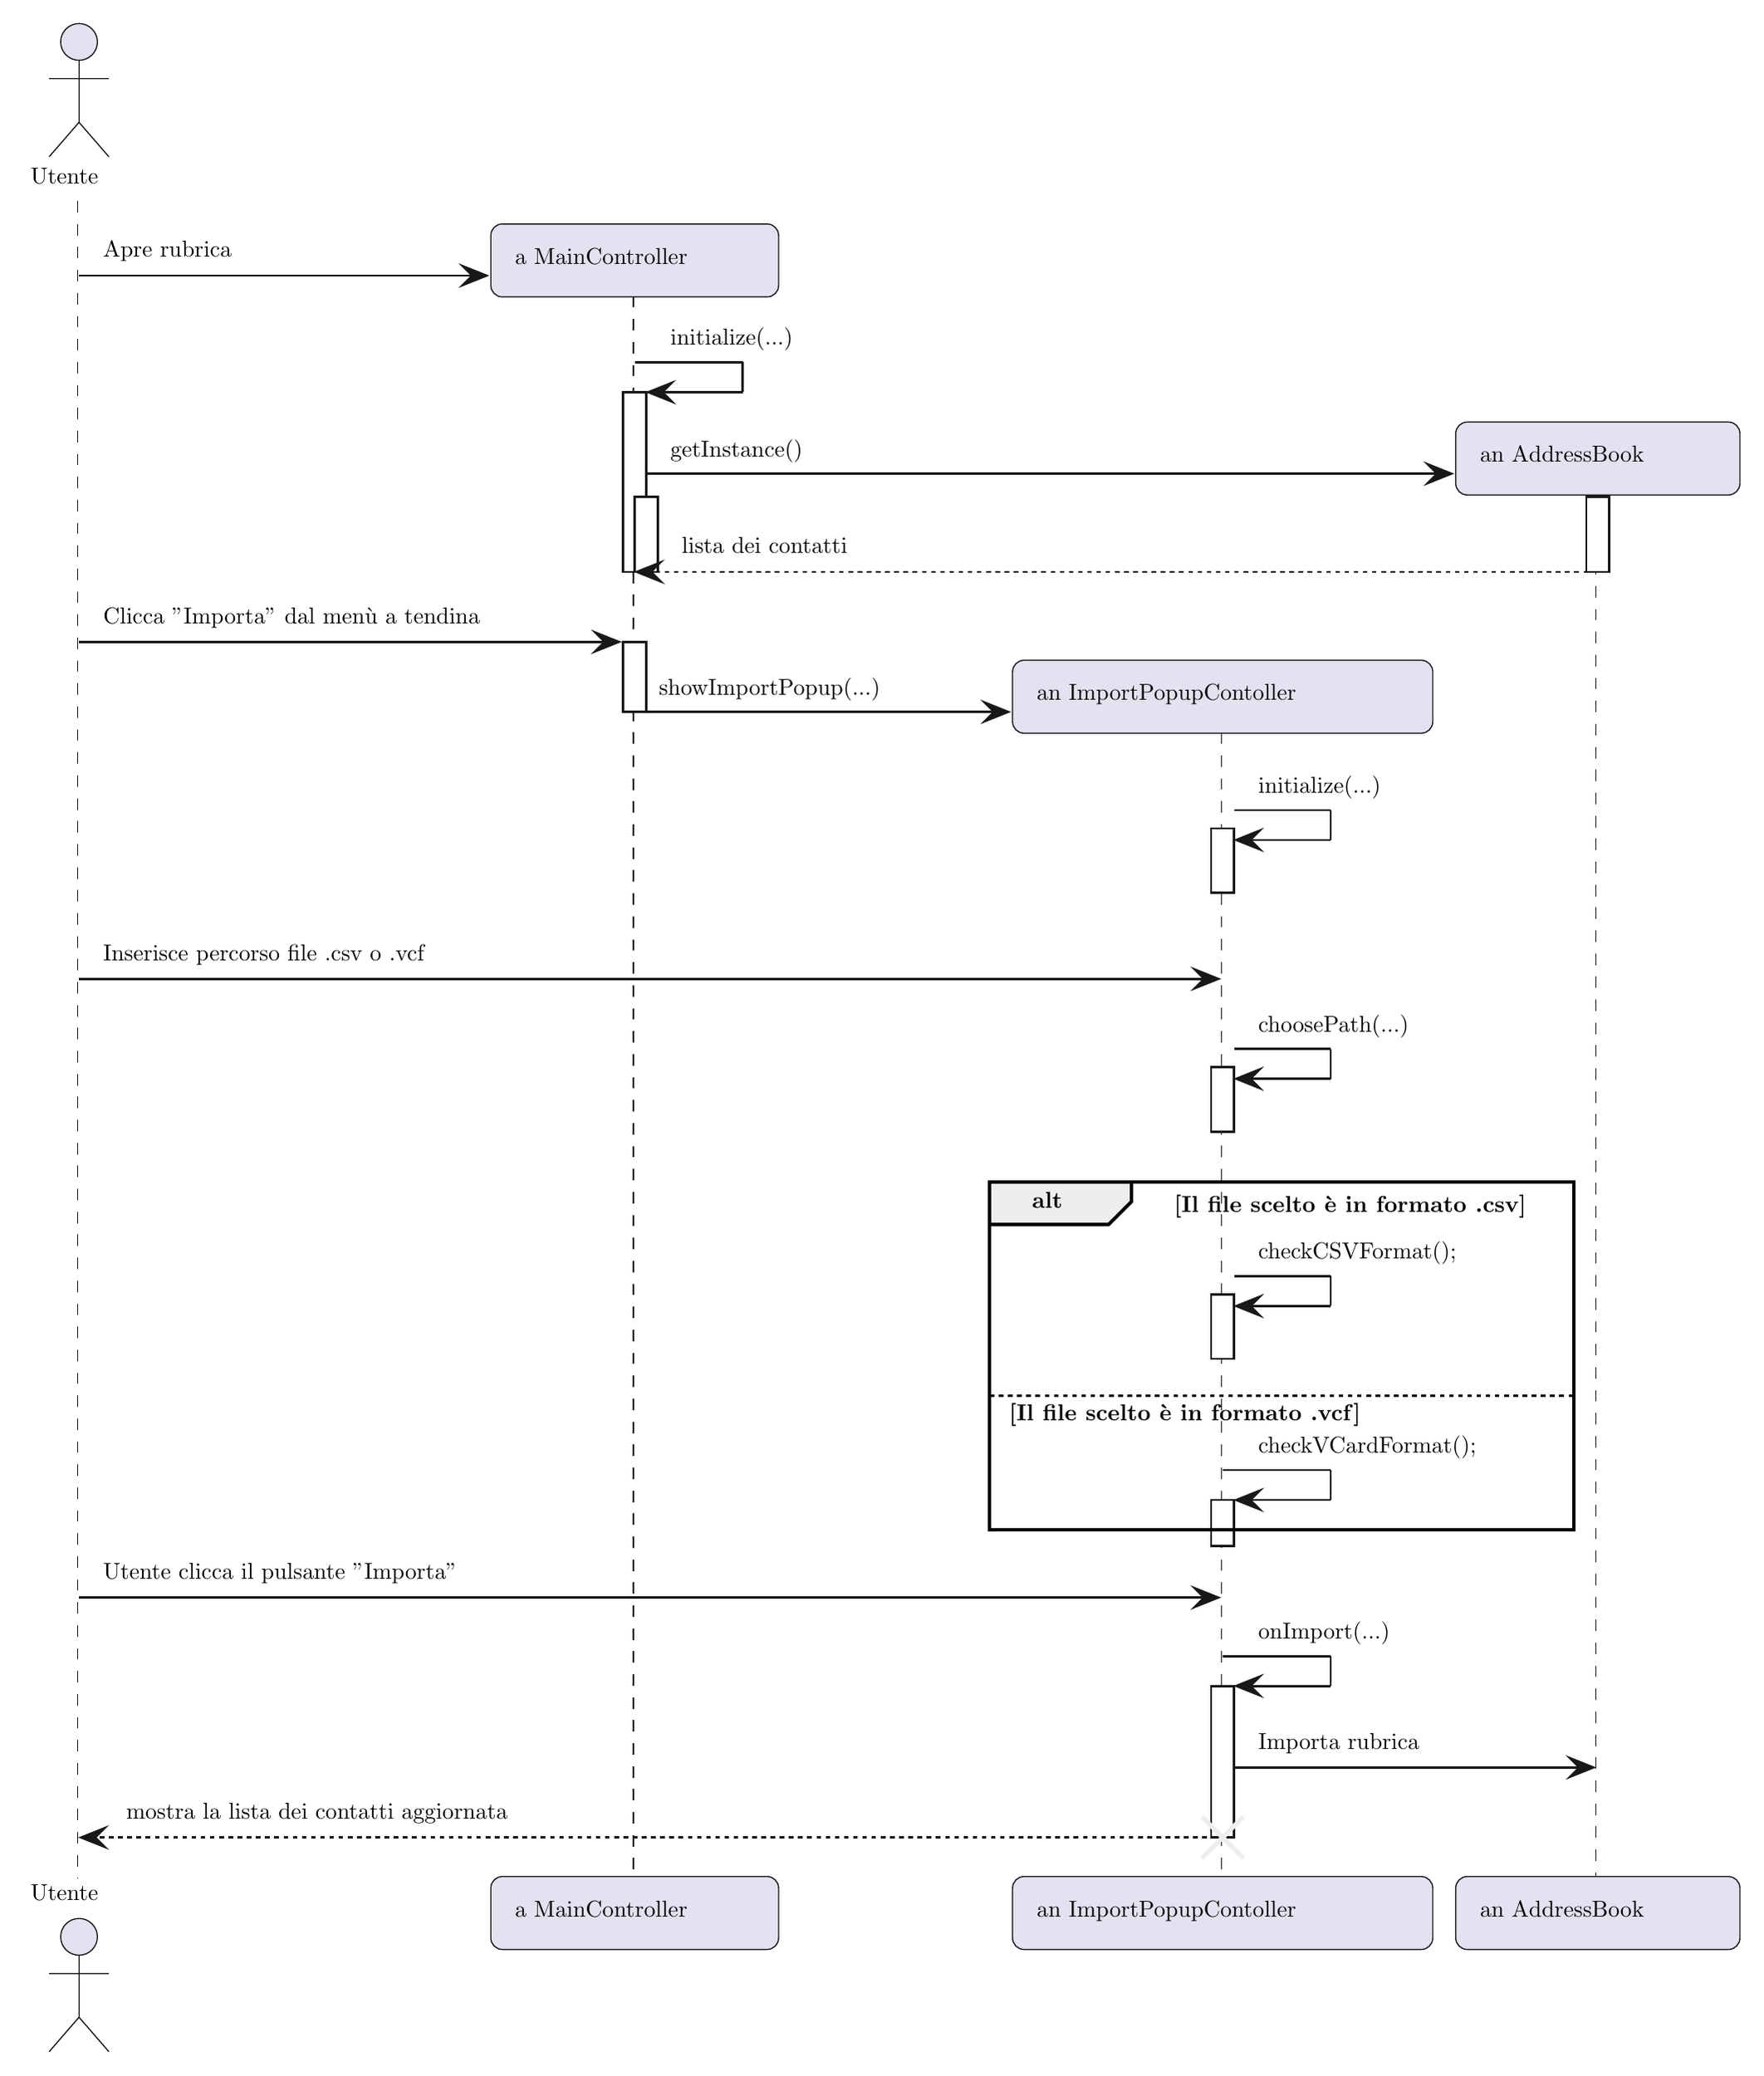
\begin{tikzpicture}[yscale=-1
,pstyle0/.style={color=plantucolor0001,fill=white,line width=1.0pt}
,pstyle1/.style={color=black,line width=1.5pt}
,pstyle2/.style={color=plantucolor0001,line width=0.5pt,dash pattern=on 5.0pt off 5.0pt}
,pstyle3/.style={color=plantucolor0001,fill=plantucolor0003,line width=0.5pt}
,pstyle4/.style={color=plantucolor0001,line width=0.5pt}
,pstyle5/.style={color=plantucolor0001,fill=plantucolor0001,line width=1.0pt}
,pstyle6/.style={color=plantucolor0001,line width=1.0pt}
,pstyle7/.style={color=plantucolor0001,line width=1.0pt,dash pattern=on 2.0pt off 2.0pt}
,pstyle10/.style={color=plantucolor0005,line width=2.0pt}
]
\draw[pstyle0] (266.4911pt,165.9707pt) rectangle (276.4911pt,244.1953pt);
\draw[pstyle0] (271.4911pt,211.4492pt) rectangle (281.4911pt,244.1953pt);
\draw[pstyle0] (266.4911pt,274.6738pt) rectangle (276.4911pt,305.1523pt);
\draw[pstyle0] (522.4243pt,355.8984pt) rectangle (532.4243pt,383.8984pt);
\draw[pstyle0] (522.4243pt,459.8555pt) rectangle (532.4243pt,487.8555pt);
\draw[pstyle0] (522.4243pt,558.8125pt) rectangle (532.4243pt,586.8125pt);
\draw[pstyle0] (522.4243pt,648.2344pt) rectangle (532.4243pt,668.2344pt);
\draw[pstyle0] (522.4243pt,729.1914pt) rectangle (532.4243pt,795.1484pt);
\draw[pstyle0] (685.7338pt,211.4492pt) rectangle (695.7338pt,244.1953pt);
\draw[pstyle1] (425.967pt,509.8555pt) rectangle (680.334pt,661.2344pt);
\draw[pstyle2] (29pt,82.7461pt) -- (29pt,813.1484pt);
\draw[pstyle2] (270.8571pt,124.1191pt) -- (270.8571pt,813.1484pt);
\draw[pstyle2] (526.967pt,314.0469pt) -- (526.967pt,813.1484pt);
\draw[pstyle2] (689.8816pt,210.3438pt) -- (689.8816pt,813.1484pt);
\node at (5pt,65pt)[below right,color=black]{Utente};
\draw[pstyle3] (29.6pt,13.5pt) ellipse (8pt and 8pt);
\draw[pstyle4] (29.6pt,21.5pt) -- (29.6pt,48.5pt)(16.6pt,29.5pt) -- (42.6pt,29.5pt)(29.6pt,48.5pt) -- (16.6pt,63.5pt)(29.6pt,48.5pt) -- (42.6pt,63.5pt);
\node at (5pt,812.1484pt)[below right,color=black]{Utente};
\draw[pstyle3] (29.6pt,838.3945pt) ellipse (8pt and 8pt);
\draw[pstyle4] (29.6pt,846.3945pt) -- (29.6pt,873.3945pt)(16.6pt,854.3945pt) -- (42.6pt,854.3945pt)(29.6pt,873.3945pt) -- (16.6pt,888.3945pt)(29.6pt,873.3945pt) -- (42.6pt,888.3945pt);
\draw[pstyle3] (208.8571pt,817.1484pt) arc (180:270:5pt) -- (213.8571pt,812.1484pt) -- (329.1251pt,812.1484pt) arc (270:360:5pt) -- (334.1251pt,817.1484pt) -- (334.1251pt,838.8945pt) arc (0:90:5pt) -- (329.1251pt,843.8945pt) -- (213.8571pt,843.8945pt) arc (90:180:5pt) -- (208.8571pt,838.8945pt) -- cycle;
\node at (215.8571pt,819.1484pt)[below right,color=black]{a MainController};
\draw[pstyle3] (435.967pt,817.1484pt) arc (180:270:5pt) -- (440.967pt,812.1484pt) -- (613.8816pt,812.1484pt) arc (270:360:5pt) -- (618.8816pt,817.1484pt) -- (618.8816pt,838.8945pt) arc (0:90:5pt) -- (613.8816pt,843.8945pt) -- (440.967pt,843.8945pt) arc (90:180:5pt) -- (435.967pt,838.8945pt) -- cycle;
\node at (442.967pt,819.1484pt)[below right,color=black]{an ImportPopupContoller};
\draw[pstyle3] (628.8816pt,817.1484pt) arc (180:270:5pt) -- (633.8816pt,812.1484pt) -- (747.586pt,812.1484pt) arc (270:360:5pt) -- (752.586pt,817.1484pt) -- (752.586pt,838.8945pt) arc (0:90:5pt) -- (747.586pt,843.8945pt) -- (633.8816pt,843.8945pt) arc (90:180:5pt) -- (628.8816pt,838.8945pt) -- cycle;
\node at (635.8816pt,819.1484pt)[below right,color=black]{an AddressBook};
\draw[pstyle0] (266.4911pt,165.9707pt) rectangle (276.4911pt,244.1953pt);
\draw[pstyle0] (271.4911pt,211.4492pt) rectangle (281.4911pt,244.1953pt);
\draw[pstyle0] (266.4911pt,274.6738pt) rectangle (276.4911pt,305.1523pt);
\draw[pstyle0] (522.4243pt,355.8984pt) rectangle (532.4243pt,383.8984pt);
\draw[pstyle0] (522.4243pt,459.8555pt) rectangle (532.4243pt,487.8555pt);
\draw[pstyle0] (522.4243pt,558.8125pt) rectangle (532.4243pt,586.8125pt);
\draw[pstyle0] (522.4243pt,648.2344pt) rectangle (532.4243pt,668.2344pt);
\draw[pstyle0] (522.4243pt,729.1914pt) rectangle (532.4243pt,795.1484pt);
\draw[pstyle0] (685.7338pt,211.4492pt) rectangle (695.7338pt,244.1953pt);
\draw[pstyle5] (196.8571pt,111.2246pt) -- (206.8571pt,115.2246pt) -- (196.8571pt,119.2246pt) -- (200.8571pt,115.2246pt) -- cycle;
\draw[pstyle6] (29.6pt,115.2246pt) -- (202.8571pt,115.2246pt);
\node at (36.6pt,96.7461pt)[below right,color=black]{Apre rubrica};
\draw[pstyle3] (208.8571pt,97.7461pt) arc (180:270:5pt) -- (213.8571pt,92.7461pt) -- (329.1251pt,92.7461pt) arc (270:360:5pt) -- (334.1251pt,97.7461pt) -- (334.1251pt,119.4922pt) arc (0:90:5pt) -- (329.1251pt,124.4922pt) -- (213.8571pt,124.4922pt) arc (90:180:5pt) -- (208.8571pt,119.4922pt) -- cycle;
\node at (215.8571pt,99.7461pt)[below right,color=black]{a MainController};
\draw[pstyle6] (271.4911pt,152.9707pt) -- (318.4911pt,152.9707pt);
\draw[pstyle6] (318.4911pt,152.9707pt) -- (318.4911pt,165.9707pt);
\draw[pstyle6] (277.4911pt,165.9707pt) -- (318.4911pt,165.9707pt);
\draw[pstyle5] (287.4911pt,161.9707pt) -- (277.4911pt,165.9707pt) -- (287.4911pt,169.9707pt) -- (283.4911pt,165.9707pt) -- cycle;
\node at (283.4911pt,134.4922pt)[below right,color=black]{initialize(...)};
\draw[pstyle5] (616.8816pt,197.4492pt) -- (626.8816pt,201.4492pt) -- (616.8816pt,205.4492pt) -- (620.8816pt,201.4492pt) -- cycle;
\draw[pstyle6] (276.4911pt,201.4492pt) -- (622.8816pt,201.4492pt);
\node at (283.4911pt,182.9707pt)[below right,color=black]{getInstance()};
\draw[pstyle3] (628.8816pt,183.9707pt) arc (180:270:5pt) -- (633.8816pt,178.9707pt) -- (747.586pt,178.9707pt) arc (270:360:5pt) -- (752.586pt,183.9707pt) -- (752.586pt,205.7168pt) arc (0:90:5pt) -- (747.586pt,210.7168pt) -- (633.8816pt,210.7168pt) arc (90:180:5pt) -- (628.8816pt,205.7168pt) -- cycle;
\node at (635.8816pt,185.9707pt)[below right,color=black]{an AddressBook};
\draw[pstyle5] (282.4911pt,240.1953pt) -- (272.4911pt,244.1953pt) -- (282.4911pt,248.1953pt) -- (278.4911pt,244.1953pt) -- cycle;
\draw[pstyle7] (276.4911pt,244.1953pt) -- (689.7338pt,244.1953pt);
\node at (288.4911pt,225.7168pt)[below right,color=black]{lista dei contatti};
\draw[pstyle5] (254.4911pt,270.6738pt) -- (264.4911pt,274.6738pt) -- (254.4911pt,278.6738pt) -- (258.4911pt,274.6738pt) -- cycle;
\draw[pstyle6] (29.6pt,274.6738pt) -- (260.4911pt,274.6738pt);
\node at (36.6pt,256.1953pt)[below right,color=black]{Clicca "Importa" dal menù a tendina};
\draw[pstyle5] (423.967pt,301.1523pt) -- (433.967pt,305.1523pt) -- (423.967pt,309.1523pt) -- (427.967pt,305.1523pt) -- cycle;
\draw[pstyle6] (271.4911pt,305.1523pt) -- (429.967pt,305.1523pt);
\node at (278.4911pt,286.6738pt)[below right,color=black]{showImportPopup(...)};
\draw[pstyle3] (435.967pt,287.6738pt) arc (180:270:5pt) -- (440.967pt,282.6738pt) -- (613.8816pt,282.6738pt) arc (270:360:5pt) -- (618.8816pt,287.6738pt) -- (618.8816pt,309.4199pt) arc (0:90:5pt) -- (613.8816pt,314.4199pt) -- (440.967pt,314.4199pt) arc (90:180:5pt) -- (435.967pt,309.4199pt) -- cycle;
\node at (442.967pt,289.6738pt)[below right,color=black]{an ImportPopupContoller};
\draw[pstyle6] (532.4243pt,347.8984pt) -- (574.4243pt,347.8984pt);
\draw[pstyle6] (574.4243pt,347.8984pt) -- (574.4243pt,360.8984pt);
\draw[pstyle6] (533.4243pt,360.8984pt) -- (574.4243pt,360.8984pt);
\draw[pstyle5] (543.4243pt,356.8984pt) -- (533.4243pt,360.8984pt) -- (543.4243pt,364.8984pt) -- (539.4243pt,360.8984pt) -- cycle;
\node at (539.4243pt,329.4199pt)[below right,color=black]{initialize(...)};
\draw[pstyle5] (515.4243pt,417.377pt) -- (525.4243pt,421.377pt) -- (515.4243pt,425.377pt) -- (519.4243pt,421.377pt) -- cycle;
\draw[pstyle6] (29.6pt,421.377pt) -- (521.4243pt,421.377pt);
\node at (36.6pt,402.8984pt)[below right,color=black]{Inserisce percorso file .csv o .vcf};
\draw[pstyle6] (532.4243pt,451.8555pt) -- (574.4243pt,451.8555pt);
\draw[pstyle6] (574.4243pt,451.8555pt) -- (574.4243pt,464.8555pt);
\draw[pstyle6] (533.4243pt,464.8555pt) -- (574.4243pt,464.8555pt);
\draw[pstyle5] (543.4243pt,460.8555pt) -- (533.4243pt,464.8555pt) -- (543.4243pt,468.8555pt) -- (539.4243pt,464.8555pt) -- cycle;
\node at (539.4243pt,433.377pt)[below right,color=black]{choosePath(...)};
\draw[color=black,fill=plantucolor0004,line width=1.5pt] (425.967pt,509.8555pt) -- (487.767pt,509.8555pt) -- (487.767pt,518.334pt) -- (477.767pt,528.334pt) -- (425.967pt,528.334pt) -- (425.967pt,509.8555pt);
\draw[pstyle1] (425.967pt,509.8555pt) rectangle (680.334pt,661.2344pt);
\node at (440.967pt,510.8555pt)[below right,color=black]{\textbf{alt}};
\node at (502.767pt,511.8555pt)[below right,color=black]{\textbf{[Il file scelto è in formato .csv]}};
\draw[pstyle6] (532.4243pt,550.8125pt) -- (574.4243pt,550.8125pt);
\draw[pstyle6] (574.4243pt,550.8125pt) -- (574.4243pt,563.8125pt);
\draw[pstyle6] (533.4243pt,563.8125pt) -- (574.4243pt,563.8125pt);
\draw[pstyle5] (543.4243pt,559.8125pt) -- (533.4243pt,563.8125pt) -- (543.4243pt,567.8125pt) -- (539.4243pt,563.8125pt) -- cycle;
\node at (539.4243pt,532.334pt)[below right,color=black]{checkCSVFormat();};
\draw[color=black,line width=1.0pt,dash pattern=on 2.0pt off 2.0pt] (425.967pt,602.8125pt) -- (680.334pt,602.8125pt);
\node at (430.967pt,602.8125pt)[below right,color=black]{\textbf{[Il file scelto è in formato .vcf]}};
\draw[pstyle6] (527.4243pt,635.2344pt) -- (574.4243pt,635.2344pt);
\draw[pstyle6] (574.4243pt,635.2344pt) -- (574.4243pt,648.2344pt);
\draw[pstyle6] (533.4243pt,648.2344pt) -- (574.4243pt,648.2344pt);
\draw[pstyle5] (543.4243pt,644.2344pt) -- (533.4243pt,648.2344pt) -- (543.4243pt,652.2344pt) -- (539.4243pt,648.2344pt) -- cycle;
\node at (539.4243pt,616.7559pt)[below right,color=black]{checkVCardFormat();};
\draw[pstyle5] (515.4243pt,686.7129pt) -- (525.4243pt,690.7129pt) -- (515.4243pt,694.7129pt) -- (519.4243pt,690.7129pt) -- cycle;
\draw[pstyle6] (29.6pt,690.7129pt) -- (521.4243pt,690.7129pt);
\node at (36.6pt,672.2344pt)[below right,color=black]{Utente clicca il pulsante "Importa"};
\draw[pstyle6] (527.4243pt,716.1914pt) -- (574.4243pt,716.1914pt);
\draw[pstyle6] (574.4243pt,716.1914pt) -- (574.4243pt,729.1914pt);
\draw[pstyle6] (533.4243pt,729.1914pt) -- (574.4243pt,729.1914pt);
\draw[pstyle5] (543.4243pt,725.1914pt) -- (533.4243pt,729.1914pt) -- (543.4243pt,733.1914pt) -- (539.4243pt,729.1914pt) -- cycle;
\node at (539.4243pt,697.7129pt)[below right,color=black]{onImport(...)};
\draw[pstyle5] (678.7338pt,760.6699pt) -- (688.7338pt,764.6699pt) -- (678.7338pt,768.6699pt) -- (682.7338pt,764.6699pt) -- cycle;
\draw[pstyle6] (532.4243pt,764.6699pt) -- (684.7338pt,764.6699pt);
\node at (539.4243pt,746.1914pt)[below right,color=black]{Importa rubrica};
\draw[pstyle5] (40.6pt,791.1484pt) -- (30.6pt,795.1484pt) -- (40.6pt,799.1484pt) -- (36.6pt,795.1484pt) -- cycle;
\draw[pstyle7] (34.6pt,795.1484pt) -- (526.4243pt,795.1484pt);
\node at (46.6pt,776.6699pt)[below right,color=black]{mostra la lista dei contatti aggiornata};
\draw[pstyle10] (518.4243pt,786.1484pt) -- (536.4243pt,804.1484pt);
\draw[pstyle10] (518.4243pt,804.1484pt) -- (536.4243pt,786.1484pt);
\end{tikzpicture}
}
\end{adjustbox}

\begin{figure}[h]
	\caption{Diagramma sequenza C5 - Importare rubrica}
	\label{fig:Diagramma sequenza C5 - Importare rubrica}
\end{figure}

\newpage
\subsubsection{C6 - Esportare rubrica}
Il seguente diagramma di sequenza illustra l'esecuzione del caso d'uso C6:
% generated by Plantuml 1.2024.3       
\definecolor{plantucolor0000}{RGB}{255,255,255}
\definecolor{plantucolor0001}{RGB}{24,24,24}
\definecolor{plantucolor0002}{RGB}{0,0,0}
\definecolor{plantucolor0003}{RGB}{226,226,240}
\definecolor{plantucolor0004}{RGB}{238,238,238}
\definecolor{plantucolor0005}{RGB}{168,0,54}

\begin{adjustbox}{width=.7\paperwidth, center}
	\resizebox{\textwidth}{!}{
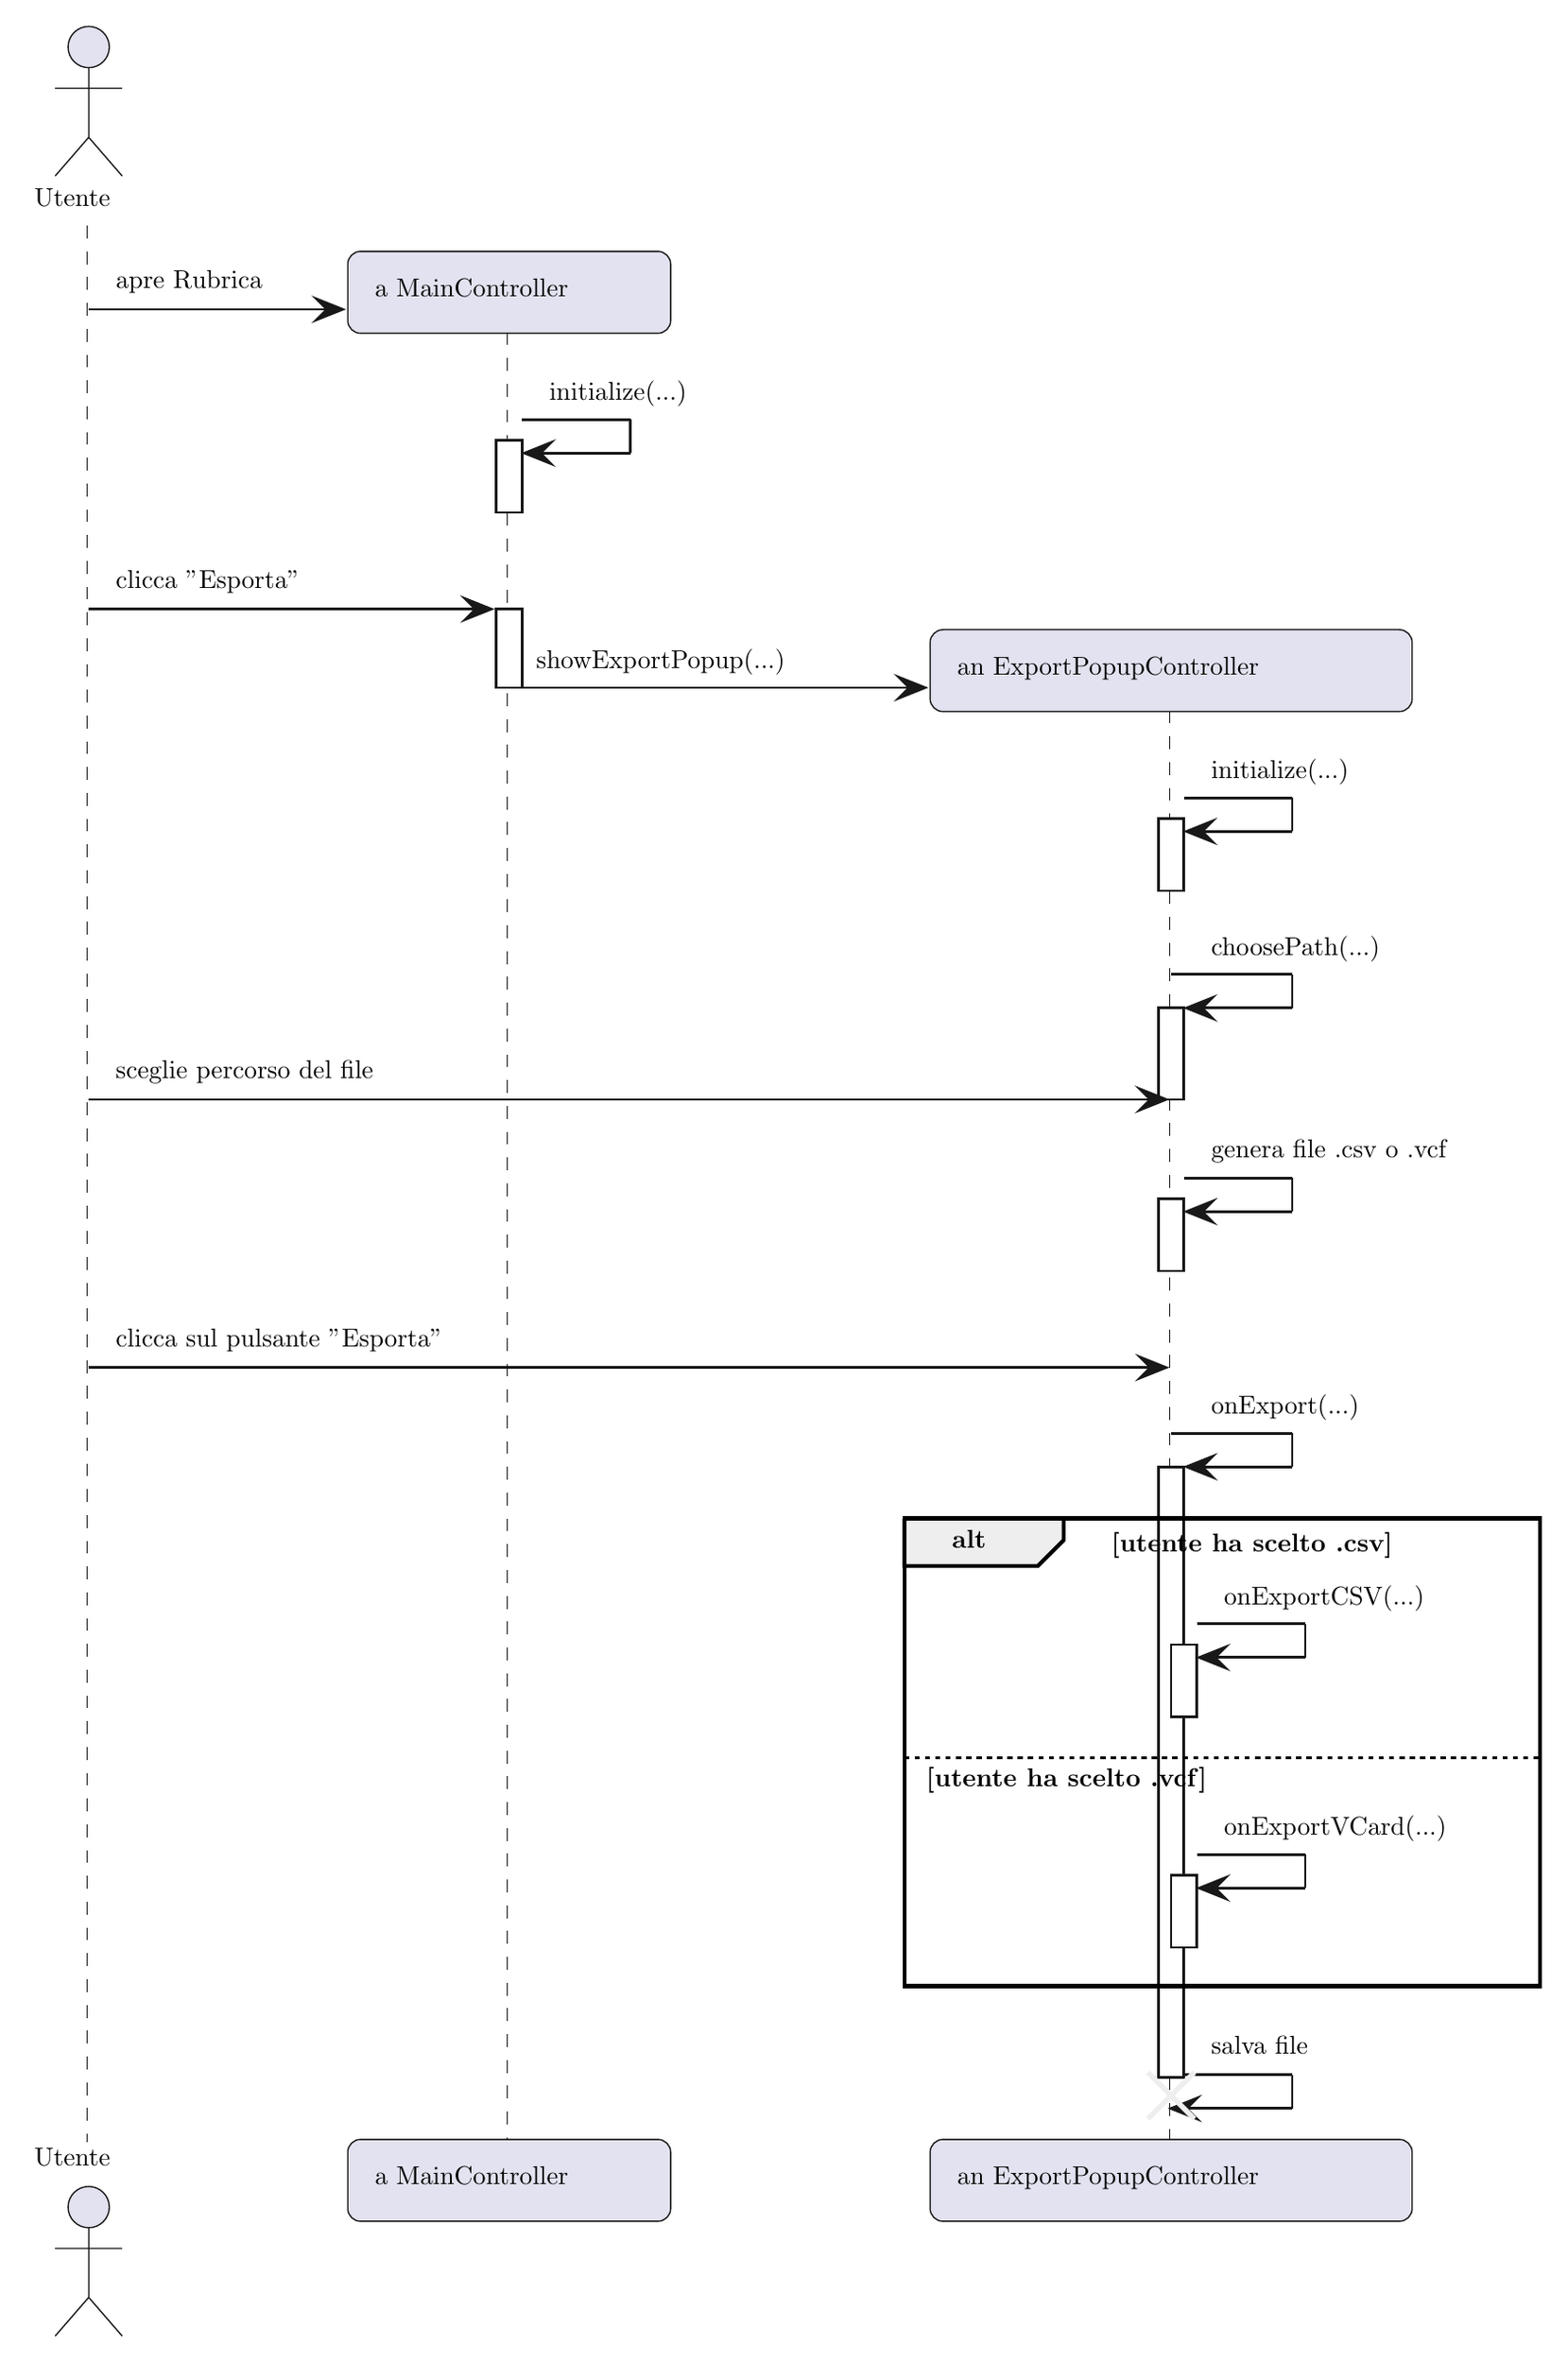
\begin{tikzpicture}[yscale=-1
,pstyle0/.style={color=plantucolor0001,fill=white,line width=1.0pt}
,pstyle1/.style={color=black,line width=1.5pt}
,pstyle2/.style={color=plantucolor0001,line width=0.5pt,dash pattern=on 5.0pt off 5.0pt}
,pstyle3/.style={color=plantucolor0001,fill=plantucolor0003,line width=0.5pt}
,pstyle4/.style={color=plantucolor0001,line width=0.5pt}
,pstyle5/.style={color=plantucolor0001,fill=plantucolor0001,line width=1.0pt}
,pstyle6/.style={color=plantucolor0001,line width=1.0pt}
,pstyle9/.style={color=plantucolor0005,line width=2.0pt}
]
\draw[pstyle0] (187.6937pt,165.9707pt) rectangle (197.6937pt,193.9707pt);
\draw[pstyle0] (187.6937pt,231.4492pt) rectangle (197.6937pt,261.9277pt);
\draw[pstyle0] (444.4229pt,312.6738pt) rectangle (454.4229pt,340.6738pt);
\draw[pstyle0] (444.4229pt,386.1523pt) rectangle (454.4229pt,421.6309pt);
\draw[pstyle0] (444.4229pt,460.1094pt) rectangle (454.4229pt,488.1094pt);
\draw[pstyle0] (444.4229pt,564.0664pt) rectangle (454.4229pt,800.9238pt);
\draw[pstyle0] (449.4229pt,633.0234pt) rectangle (459.4229pt,661.0234pt);
\draw[pstyle0] (449.4229pt,722.4453pt) rectangle (459.4229pt,750.4453pt);
\draw[pstyle1] (345.9372pt,584.0664pt) rectangle (592.5535pt,765.4453pt);
\draw[pstyle2] (29pt,82.7461pt) -- (29pt,825.9238pt);
\draw[pstyle2] (192.0597pt,124.1191pt) -- (192.0597pt,825.9238pt);
\draw[pstyle2] (448.9372pt,270.8223pt) -- (448.9372pt,825.9238pt);
\node at (5pt,65pt)[below right,color=black]{Utente};
\draw[pstyle3] (29.6pt,13.5pt) ellipse (8pt and 8pt);
\draw[pstyle4] (29.6pt,21.5pt) -- (29.6pt,48.5pt)(16.6pt,29.5pt) -- (42.6pt,29.5pt)(29.6pt,48.5pt) -- (16.6pt,63.5pt)(29.6pt,48.5pt) -- (42.6pt,63.5pt);
\node at (5pt,824.9238pt)[below right,color=black]{Utente};
\draw[pstyle3] (29.6pt,851.1699pt) ellipse (8pt and 8pt);
\draw[pstyle4] (29.6pt,859.1699pt) -- (29.6pt,886.1699pt)(16.6pt,867.1699pt) -- (42.6pt,867.1699pt)(29.6pt,886.1699pt) -- (16.6pt,901.1699pt)(29.6pt,886.1699pt) -- (42.6pt,901.1699pt);
\draw[pstyle3] (130.0597pt,829.9238pt) arc (180:270:5pt) -- (135.0597pt,824.9238pt) -- (250.3278pt,824.9238pt) arc (270:360:5pt) -- (255.3278pt,829.9238pt) -- (255.3278pt,851.6699pt) arc (0:90:5pt) -- (250.3278pt,856.6699pt) -- (135.0597pt,856.6699pt) arc (90:180:5pt) -- (130.0597pt,851.6699pt) -- cycle;
\node at (137.0597pt,831.9238pt)[below right,color=black]{a MainController};
\draw[pstyle3] (355.9372pt,829.9238pt) arc (180:270:5pt) -- (360.9372pt,824.9238pt) -- (537.9087pt,824.9238pt) arc (270:360:5pt) -- (542.9087pt,829.9238pt) -- (542.9087pt,851.6699pt) arc (0:90:5pt) -- (537.9087pt,856.6699pt) -- (360.9372pt,856.6699pt) arc (90:180:5pt) -- (355.9372pt,851.6699pt) -- cycle;
\node at (362.9372pt,831.9238pt)[below right,color=black]{an ExportPopupController};
\draw[pstyle0] (187.6937pt,165.9707pt) rectangle (197.6937pt,193.9707pt);
\draw[pstyle0] (187.6937pt,231.4492pt) rectangle (197.6937pt,261.9277pt);
\draw[pstyle0] (444.4229pt,312.6738pt) rectangle (454.4229pt,340.6738pt);
\draw[pstyle0] (444.4229pt,386.1523pt) rectangle (454.4229pt,421.6309pt);
\draw[pstyle0] (444.4229pt,460.1094pt) rectangle (454.4229pt,488.1094pt);
\draw[pstyle0] (444.4229pt,564.0664pt) rectangle (454.4229pt,800.9238pt);
\draw[pstyle0] (449.4229pt,633.0234pt) rectangle (459.4229pt,661.0234pt);
\draw[pstyle0] (449.4229pt,722.4453pt) rectangle (459.4229pt,750.4453pt);
\draw[pstyle5] (118.0597pt,111.2246pt) -- (128.0597pt,115.2246pt) -- (118.0597pt,119.2246pt) -- (122.0597pt,115.2246pt) -- cycle;
\draw[pstyle6] (29.6pt,115.2246pt) -- (124.0597pt,115.2246pt);
\node at (36.6pt,96.7461pt)[below right,color=black]{apre Rubrica};
\draw[pstyle3] (130.0597pt,97.7461pt) arc (180:270:5pt) -- (135.0597pt,92.7461pt) -- (250.3278pt,92.7461pt) arc (270:360:5pt) -- (255.3278pt,97.7461pt) -- (255.3278pt,119.4922pt) arc (0:90:5pt) -- (250.3278pt,124.4922pt) -- (135.0597pt,124.4922pt) arc (90:180:5pt) -- (130.0597pt,119.4922pt) -- cycle;
\node at (137.0597pt,99.7461pt)[below right,color=black]{a MainController};
\draw[pstyle6] (197.6937pt,157.9707pt) -- (239.6937pt,157.9707pt);
\draw[pstyle6] (239.6937pt,157.9707pt) -- (239.6937pt,170.9707pt);
\draw[pstyle6] (198.6937pt,170.9707pt) -- (239.6937pt,170.9707pt);
\draw[pstyle5] (208.6937pt,166.9707pt) -- (198.6937pt,170.9707pt) -- (208.6937pt,174.9707pt) -- (204.6937pt,170.9707pt) -- cycle;
\node at (204.6937pt,139.4922pt)[below right,color=black]{initialize(...)};
\draw[pstyle5] (175.6937pt,227.4492pt) -- (185.6937pt,231.4492pt) -- (175.6937pt,235.4492pt) -- (179.6937pt,231.4492pt) -- cycle;
\draw[pstyle6] (29.6pt,231.4492pt) -- (181.6937pt,231.4492pt);
\node at (36.6pt,212.9707pt)[below right,color=black]{clicca "Esporta"};
\draw[pstyle5] (343.9372pt,257.9277pt) -- (353.9372pt,261.9277pt) -- (343.9372pt,265.9277pt) -- (347.9372pt,261.9277pt) -- cycle;
\draw[pstyle6] (192.6937pt,261.9277pt) -- (349.9372pt,261.9277pt);
\node at (199.6937pt,243.4492pt)[below right,color=black]{showExportPopup(...)};
\draw[pstyle3] (355.9372pt,244.4492pt) arc (180:270:5pt) -- (360.9372pt,239.4492pt) -- (537.9087pt,239.4492pt) arc (270:360:5pt) -- (542.9087pt,244.4492pt) -- (542.9087pt,266.1953pt) arc (0:90:5pt) -- (537.9087pt,271.1953pt) -- (360.9372pt,271.1953pt) arc (90:180:5pt) -- (355.9372pt,266.1953pt) -- cycle;
\node at (362.9372pt,246.4492pt)[below right,color=black]{an ExportPopupController};
\draw[pstyle6] (454.4229pt,304.6738pt) -- (496.4229pt,304.6738pt);
\draw[pstyle6] (496.4229pt,304.6738pt) -- (496.4229pt,317.6738pt);
\draw[pstyle6] (455.4229pt,317.6738pt) -- (496.4229pt,317.6738pt);
\draw[pstyle5] (465.4229pt,313.6738pt) -- (455.4229pt,317.6738pt) -- (465.4229pt,321.6738pt) -- (461.4229pt,317.6738pt) -- cycle;
\node at (461.4229pt,286.1953pt)[below right,color=black]{initialize(...)};
\draw[pstyle6] (449.4229pt,373.1523pt) -- (496.4229pt,373.1523pt);
\draw[pstyle6] (496.4229pt,373.1523pt) -- (496.4229pt,386.1523pt);
\draw[pstyle6] (455.4229pt,386.1523pt) -- (496.4229pt,386.1523pt);
\draw[pstyle5] (465.4229pt,382.1523pt) -- (455.4229pt,386.1523pt) -- (465.4229pt,390.1523pt) -- (461.4229pt,386.1523pt) -- cycle;
\node at (461.4229pt,354.6738pt)[below right,color=black]{choosePath(...)};
\draw[pstyle5] (437.4229pt,417.6309pt) -- (447.4229pt,421.6309pt) -- (437.4229pt,425.6309pt) -- (441.4229pt,421.6309pt) -- cycle;
\draw[pstyle6] (29.6pt,421.6309pt) -- (443.4229pt,421.6309pt);
\node at (36.6pt,403.1523pt)[below right,color=black]{sceglie percorso del file};
\draw[pstyle6] (454.4229pt,452.1094pt) -- (496.4229pt,452.1094pt);
\draw[pstyle6] (496.4229pt,452.1094pt) -- (496.4229pt,465.1094pt);
\draw[pstyle6] (455.4229pt,465.1094pt) -- (496.4229pt,465.1094pt);
\draw[pstyle5] (465.4229pt,461.1094pt) -- (455.4229pt,465.1094pt) -- (465.4229pt,469.1094pt) -- (461.4229pt,465.1094pt) -- cycle;
\node at (461.4229pt,433.6309pt)[below right,color=black]{genera file .csv o .vcf};
\draw[pstyle5] (437.4229pt,521.5879pt) -- (447.4229pt,525.5879pt) -- (437.4229pt,529.5879pt) -- (441.4229pt,525.5879pt) -- cycle;
\draw[pstyle6] (29.6pt,525.5879pt) -- (443.4229pt,525.5879pt);
\node at (36.6pt,507.1094pt)[below right,color=black]{clicca sul pulsante "Esporta"};
\draw[pstyle6] (449.4229pt,551.0664pt) -- (496.4229pt,551.0664pt);
\draw[pstyle6] (496.4229pt,551.0664pt) -- (496.4229pt,564.0664pt);
\draw[pstyle6] (455.4229pt,564.0664pt) -- (496.4229pt,564.0664pt);
\draw[pstyle5] (465.4229pt,560.0664pt) -- (455.4229pt,564.0664pt) -- (465.4229pt,568.0664pt) -- (461.4229pt,564.0664pt) -- cycle;
\node at (461.4229pt,532.5879pt)[below right,color=black]{onExport(...)};
\draw[color=black,fill=plantucolor0004,line width=1.5pt] (345.9372pt,584.0664pt) -- (407.7372pt,584.0664pt) -- (407.7372pt,592.5449pt) -- (397.7372pt,602.5449pt) -- (345.9372pt,602.5449pt) -- (345.9372pt,584.0664pt);
\draw[pstyle1] (345.9372pt,584.0664pt) rectangle (592.5535pt,765.4453pt);
\node at (360.9372pt,585.0664pt)[below right,color=black]{\textbf{alt}};
\node at (422.7372pt,586.0664pt)[below right,color=black]{\textbf{[utente ha scelto .csv]}};
\draw[pstyle6] (459.4229pt,625.0234pt) -- (501.4229pt,625.0234pt);
\draw[pstyle6] (501.4229pt,625.0234pt) -- (501.4229pt,638.0234pt);
\draw[pstyle6] (460.4229pt,638.0234pt) -- (501.4229pt,638.0234pt);
\draw[pstyle5] (470.4229pt,634.0234pt) -- (460.4229pt,638.0234pt) -- (470.4229pt,642.0234pt) -- (466.4229pt,638.0234pt) -- cycle;
\node at (466.4229pt,606.5449pt)[below right,color=black]{onExportCSV(...)};
\draw[color=black,line width=1.0pt,dash pattern=on 2.0pt off 2.0pt] (345.9372pt,677.0234pt) -- (592.5535pt,677.0234pt);
\node at (350.9372pt,677.0234pt)[below right,color=black]{\textbf{[utente ha scelto .vcf]}};
\draw[pstyle6] (459.4229pt,714.4453pt) -- (501.4229pt,714.4453pt);
\draw[pstyle6] (501.4229pt,714.4453pt) -- (501.4229pt,727.4453pt);
\draw[pstyle6] (460.4229pt,727.4453pt) -- (501.4229pt,727.4453pt);
\draw[pstyle5] (470.4229pt,723.4453pt) -- (460.4229pt,727.4453pt) -- (470.4229pt,731.4453pt) -- (466.4229pt,727.4453pt) -- cycle;
\node at (466.4229pt,695.9668pt)[below right,color=black]{onExportVCard(...)};
\draw[pstyle6] (454.4229pt,799.9238pt) -- (496.4229pt,799.9238pt);
\draw[pstyle6] (496.4229pt,799.9238pt) -- (496.4229pt,812.9238pt);
\draw[pstyle6] (449.4229pt,812.9238pt) -- (496.4229pt,812.9238pt);
\draw[pstyle5] (459.4229pt,808.9238pt) -- (449.4229pt,812.9238pt) -- (459.4229pt,816.9238pt) -- (455.4229pt,812.9238pt) -- cycle;
\node at (461.4229pt,781.4453pt)[below right,color=black]{salva file};
\draw[pstyle9] (440.4229pt,798.9238pt) -- (458.4229pt,816.9238pt);
\draw[pstyle9] (440.4229pt,816.9238pt) -- (458.4229pt,798.9238pt);
\end{tikzpicture}
}
\end{adjustbox}

\begin{figure}[h]
	\caption{Diagramma sequenza C6 - Esportare rubrica}
	\label{fig:Diagramma sequenza C6 - Esportare rubrica}
\end{figure}

\newpage
\subsubsection{C8 - Salvare rubrica}
Il seguente diagramma di sequenza illustra l'esecuzione del caso d'uso C8:
% generated by Plantuml 1.2024.3       
\definecolor{plantucolor0000}{RGB}{255,255,255}
\definecolor{plantucolor0001}{RGB}{24,24,24}
\definecolor{plantucolor0002}{RGB}{0,0,0}
\definecolor{plantucolor0003}{RGB}{226,226,240}
\definecolor{plantucolor0004}{RGB}{254,255,221}
\definecolor{plantucolor0005}{RGB}{238,238,238}

\begin{adjustbox}{width=.9\paperwidth, center}
	\resizebox{\textwidth}{!}{
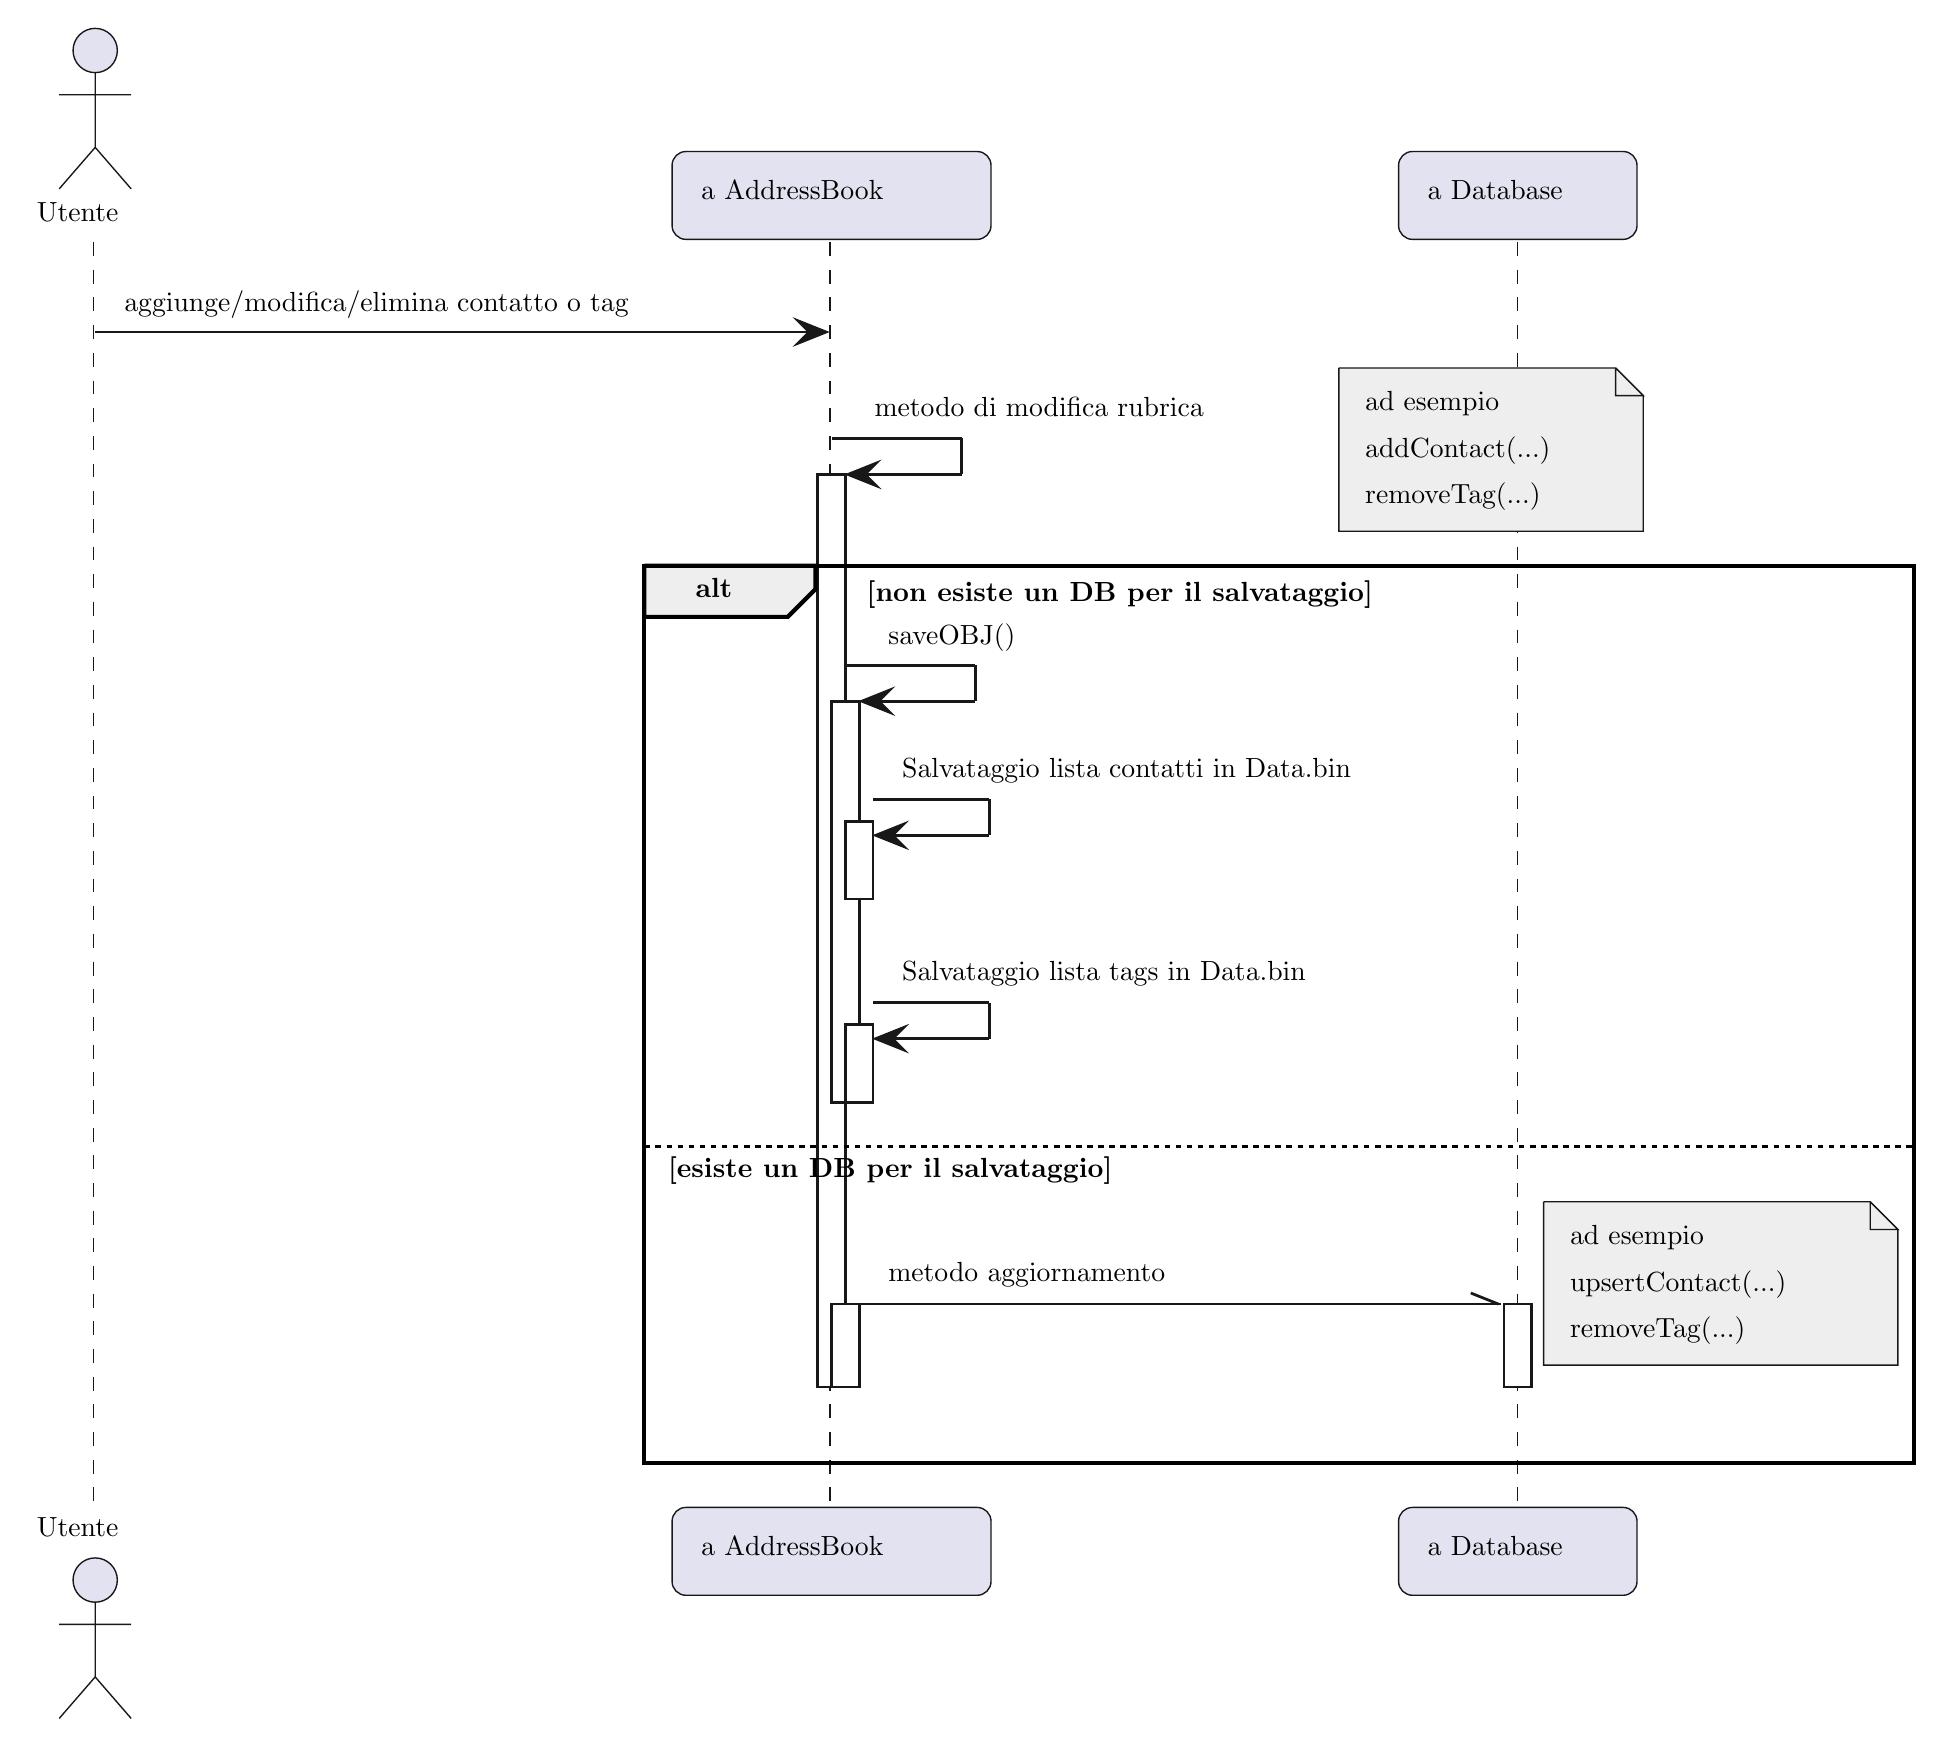
\begin{tikzpicture}[yscale=-1
,pstyle0/.style={color=plantucolor0001,fill=white,line width=1.0pt}
,pstyle1/.style={color=black,line width=1.5pt}
,pstyle2/.style={color=plantucolor0001,line width=0.5pt,dash pattern=on 5.0pt off 5.0pt}
,pstyle3/.style={color=plantucolor0001,fill=plantucolor0003,line width=0.5pt}
,pstyle4/.style={color=plantucolor0001,line width=0.5pt}
,pstyle5/.style={color=plantucolor0001,fill=plantucolor0001,line width=1.0pt}
,pstyle6/.style={color=plantucolor0001,line width=1.0pt}
,pstyle7/.style={color=plantucolor0001,fill=plantucolor0004,line width=0.5pt}
]
\draw[pstyle0] (290.6771pt,166.6816pt) rectangle (300.6771pt,496.4746pt);
\draw[pstyle0] (295.6771pt,248.6172pt) rectangle (305.6771pt,393.5742pt);
\draw[pstyle0] (300.6771pt,292.0957pt) rectangle (310.6771pt,320.0957pt);
\draw[pstyle0] (300.6771pt,365.5742pt) rectangle (310.6771pt,393.5742pt);
\draw[pstyle0] (295.6771pt,466.4746pt) rectangle (305.6771pt,496.4746pt);
\draw[pstyle0] (538.6553pt,466.4746pt) rectangle (548.6553pt,496.4746pt);
\draw[pstyle1] (228.0535pt,199.6602pt) rectangle (686.7392pt,523.9531pt);
\draw[pstyle2] (29pt,82.7461pt) -- (29pt,540.9531pt);
\draw[pstyle2] (295.0535pt,82.7461pt) -- (295.0535pt,540.9531pt);
\draw[pstyle2] (543.5799pt,82.7461pt) -- (543.5799pt,540.9531pt);
\node at (5pt,65pt)[below right,color=black]{Utente};
\draw[pstyle3] (29.6pt,13.5pt) ellipse (8pt and 8pt);
\draw[pstyle4] (29.6pt,21.5pt) -- (29.6pt,48.5pt)(16.6pt,29.5pt) -- (42.6pt,29.5pt)(29.6pt,48.5pt) -- (16.6pt,63.5pt)(29.6pt,48.5pt) -- (42.6pt,63.5pt);
\node at (5pt,539.9531pt)[below right,color=black]{Utente};
\draw[pstyle3] (29.6pt,566.1992pt) ellipse (8pt and 8pt);
\draw[pstyle4] (29.6pt,574.1992pt) -- (29.6pt,601.1992pt)(16.6pt,582.1992pt) -- (42.6pt,582.1992pt)(29.6pt,601.1992pt) -- (16.6pt,616.1992pt)(29.6pt,601.1992pt) -- (42.6pt,616.1992pt);
\draw[pstyle3] (238.0535pt,55pt) arc (180:270:5pt) -- (243.0535pt,50pt) -- (348.3006pt,50pt) arc (270:360:5pt) -- (353.3006pt,55pt) -- (353.3006pt,76.7461pt) arc (0:90:5pt) -- (348.3006pt,81.7461pt) -- (243.0535pt,81.7461pt) arc (90:180:5pt) -- (238.0535pt,76.7461pt) -- cycle;
\node at (245.0535pt,57pt)[below right,color=black]{a AddressBook};
\draw[pstyle3] (238.0535pt,544.9531pt) arc (180:270:5pt) -- (243.0535pt,539.9531pt) -- (348.3006pt,539.9531pt) arc (270:360:5pt) -- (353.3006pt,544.9531pt) -- (353.3006pt,566.6992pt) arc (0:90:5pt) -- (348.3006pt,571.6992pt) -- (243.0535pt,571.6992pt) arc (90:180:5pt) -- (238.0535pt,566.6992pt) -- cycle;
\node at (245.0535pt,546.9531pt)[below right,color=black]{a AddressBook};
\draw[pstyle3] (500.5799pt,55pt) arc (180:270:5pt) -- (505.5799pt,50pt) -- (581.7307pt,50pt) arc (270:360:5pt) -- (586.7307pt,55pt) -- (586.7307pt,76.7461pt) arc (0:90:5pt) -- (581.7307pt,81.7461pt) -- (505.5799pt,81.7461pt) arc (90:180:5pt) -- (500.5799pt,76.7461pt) -- cycle;
\node at (507.5799pt,57pt)[below right,color=black]{a Database};
\draw[pstyle3] (500.5799pt,544.9531pt) arc (180:270:5pt) -- (505.5799pt,539.9531pt) -- (581.7307pt,539.9531pt) arc (270:360:5pt) -- (586.7307pt,544.9531pt) -- (586.7307pt,566.6992pt) arc (0:90:5pt) -- (581.7307pt,571.6992pt) -- (505.5799pt,571.6992pt) arc (90:180:5pt) -- (500.5799pt,566.6992pt) -- cycle;
\node at (507.5799pt,546.9531pt)[below right,color=black]{a Database};
\draw[pstyle0] (290.6771pt,166.6816pt) rectangle (300.6771pt,496.4746pt);
\draw[pstyle0] (295.6771pt,248.6172pt) rectangle (305.6771pt,393.5742pt);
\draw[pstyle0] (300.6771pt,292.0957pt) rectangle (310.6771pt,320.0957pt);
\draw[pstyle0] (300.6771pt,365.5742pt) rectangle (310.6771pt,393.5742pt);
\draw[pstyle0] (295.6771pt,466.4746pt) rectangle (305.6771pt,496.4746pt);
\draw[pstyle0] (538.6553pt,466.4746pt) rectangle (548.6553pt,496.4746pt);
\draw[pstyle5] (283.6771pt,111.2246pt) -- (293.6771pt,115.2246pt) -- (283.6771pt,119.2246pt) -- (287.6771pt,115.2246pt) -- cycle;
\draw[pstyle6] (29.6pt,115.2246pt) -- (289.6771pt,115.2246pt);
\node at (36.6pt,96.7461pt)[below right,color=black]{aggiunge/modifica/elimina contatto o tag};
\draw[pstyle6] (295.6771pt,153.6816pt) -- (342.6771pt,153.6816pt);
\draw[pstyle6] (342.6771pt,153.6816pt) -- (342.6771pt,166.6816pt);
\draw[pstyle6] (301.6771pt,166.6816pt) -- (342.6771pt,166.6816pt);
\draw[pstyle5] (311.6771pt,162.6816pt) -- (301.6771pt,166.6816pt) -- (311.6771pt,170.6816pt) -- (307.6771pt,166.6816pt) -- cycle;
\node at (307.6771pt,135.2031pt)[below right,color=black]{metodo di modifica rubrica};
\draw[pstyle7] (478.9801pt,128.2246pt) -- (478.9801pt,187.2246pt) -- (588.9801pt,187.2246pt) -- (588.9801pt,138.2246pt) -- (578.9801pt,128.2246pt) -- (478.9801pt,128.2246pt);
\draw[pstyle7] (578.9801pt,128.2246pt) -- (578.9801pt,138.2246pt) -- (588.9801pt,138.2246pt) -- (578.9801pt,128.2246pt);
\node at (484.9801pt,133.2246pt)[below right,color=black]{ad esempio};
\node at (484.9801pt,149.7031pt)[below right,color=black]{addContact(...)};
\node at (484.9801pt,166.1816pt)[below right,color=black]{removeTag(...)};
\draw[color=black,fill=plantucolor0005,line width=1.5pt] (228.0535pt,199.6602pt) -- (289.8535pt,199.6602pt) -- (289.8535pt,208.1387pt) -- (279.8535pt,218.1387pt) -- (228.0535pt,218.1387pt) -- (228.0535pt,199.6602pt);
\draw[pstyle1] (228.0535pt,199.6602pt) rectangle (686.7392pt,523.9531pt);
\node at (243.0535pt,200.6602pt)[below right,color=black]{\textbf{alt}};
\node at (304.8535pt,201.6602pt)[below right,color=black]{\textbf{[non esiste un DB per il salvataggio]}};
\draw[pstyle6] (300.6771pt,235.6172pt) -- (347.6771pt,235.6172pt);
\draw[pstyle6] (347.6771pt,235.6172pt) -- (347.6771pt,248.6172pt);
\draw[pstyle6] (306.6771pt,248.6172pt) -- (347.6771pt,248.6172pt);
\draw[pstyle5] (316.6771pt,244.6172pt) -- (306.6771pt,248.6172pt) -- (316.6771pt,252.6172pt) -- (312.6771pt,248.6172pt) -- cycle;
\node at (312.6771pt,217.1387pt)[below right,color=black]{saveOBJ()};
\draw[pstyle6] (310.6771pt,284.0957pt) -- (352.6771pt,284.0957pt);
\draw[pstyle6] (352.6771pt,284.0957pt) -- (352.6771pt,297.0957pt);
\draw[pstyle6] (311.6771pt,297.0957pt) -- (352.6771pt,297.0957pt);
\draw[pstyle5] (321.6771pt,293.0957pt) -- (311.6771pt,297.0957pt) -- (321.6771pt,301.0957pt) -- (317.6771pt,297.0957pt) -- cycle;
\node at (317.6771pt,265.6172pt)[below right,color=black]{Salvataggio lista contatti in Data.bin};
\draw[pstyle6] (310.6771pt,357.5742pt) -- (352.6771pt,357.5742pt);
\draw[pstyle6] (352.6771pt,357.5742pt) -- (352.6771pt,370.5742pt);
\draw[pstyle6] (311.6771pt,370.5742pt) -- (352.6771pt,370.5742pt);
\draw[pstyle5] (321.6771pt,366.5742pt) -- (311.6771pt,370.5742pt) -- (321.6771pt,374.5742pt) -- (317.6771pt,370.5742pt) -- cycle;
\node at (317.6771pt,339.0957pt)[below right,color=black]{Salvataggio lista tags in Data.bin};
\draw[color=black,line width=1.0pt,dash pattern=on 2.0pt off 2.0pt] (228.0535pt,409.5742pt) -- (686.7392pt,409.5742pt);
\node at (233.0535pt,409.5742pt)[below right,color=black]{\textbf{[esiste un DB per il salvataggio]}};
\draw[pstyle6] (536.6553pt,466.4746pt) -- (526.6553pt,462.4746pt);
\draw[pstyle6] (305.6771pt,466.4746pt) -- (537.6553pt,466.4746pt);
\node at (312.6771pt,447.9961pt)[below right,color=black]{metodo aggiornamento};
\draw[pstyle7] (553pt,429.5176pt) -- (553pt,488.5176pt) -- (681pt,488.5176pt) -- (681pt,439.5176pt) -- (671pt,429.5176pt) -- (553pt,429.5176pt);
\draw[pstyle7] (671pt,429.5176pt) -- (671pt,439.5176pt) -- (681pt,439.5176pt) -- (671pt,429.5176pt);
\node at (559pt,434.5176pt)[below right,color=black]{ad esempio};
\node at (559pt,450.9961pt)[below right,color=black]{upsertContact(...)};
\node at (559pt,467.4746pt)[below right,color=black]{removeTag(...)};
\end{tikzpicture}
}
\end{adjustbox}

\begin{figure}[h]
	\caption{Diagramma sequenza C8 - Salvare rubrica}
	\label{fig:Diagramma sequenza C8 - Salvare rubrica}
\end{figure}

\newpage
\subsubsection{Aggiunta DB}
Il seguente diagramma di sequenza illustra il flusso di operazioni attraverso cui l'utente aggiunge un link a un Database, consentendo il salvataggio dei dati nel DB anziché in locale.:
% generated by Plantuml 1.2024.3       
\definecolor{plantucolor0000}{RGB}{255,255,255}
\definecolor{plantucolor0001}{RGB}{24,24,24}
\definecolor{plantucolor0002}{RGB}{0,0,0}
\definecolor{plantucolor0003}{RGB}{226,226,240}
\definecolor{plantucolor0004}{RGB}{254,255,221}
\definecolor{plantucolor0005}{RGB}{238,238,238}
\definecolor{plantucolor0006}{RGB}{168,0,54}

\begin{adjustbox}{width=.9\paperwidth, center}
	\resizebox{\textwidth}{!}{
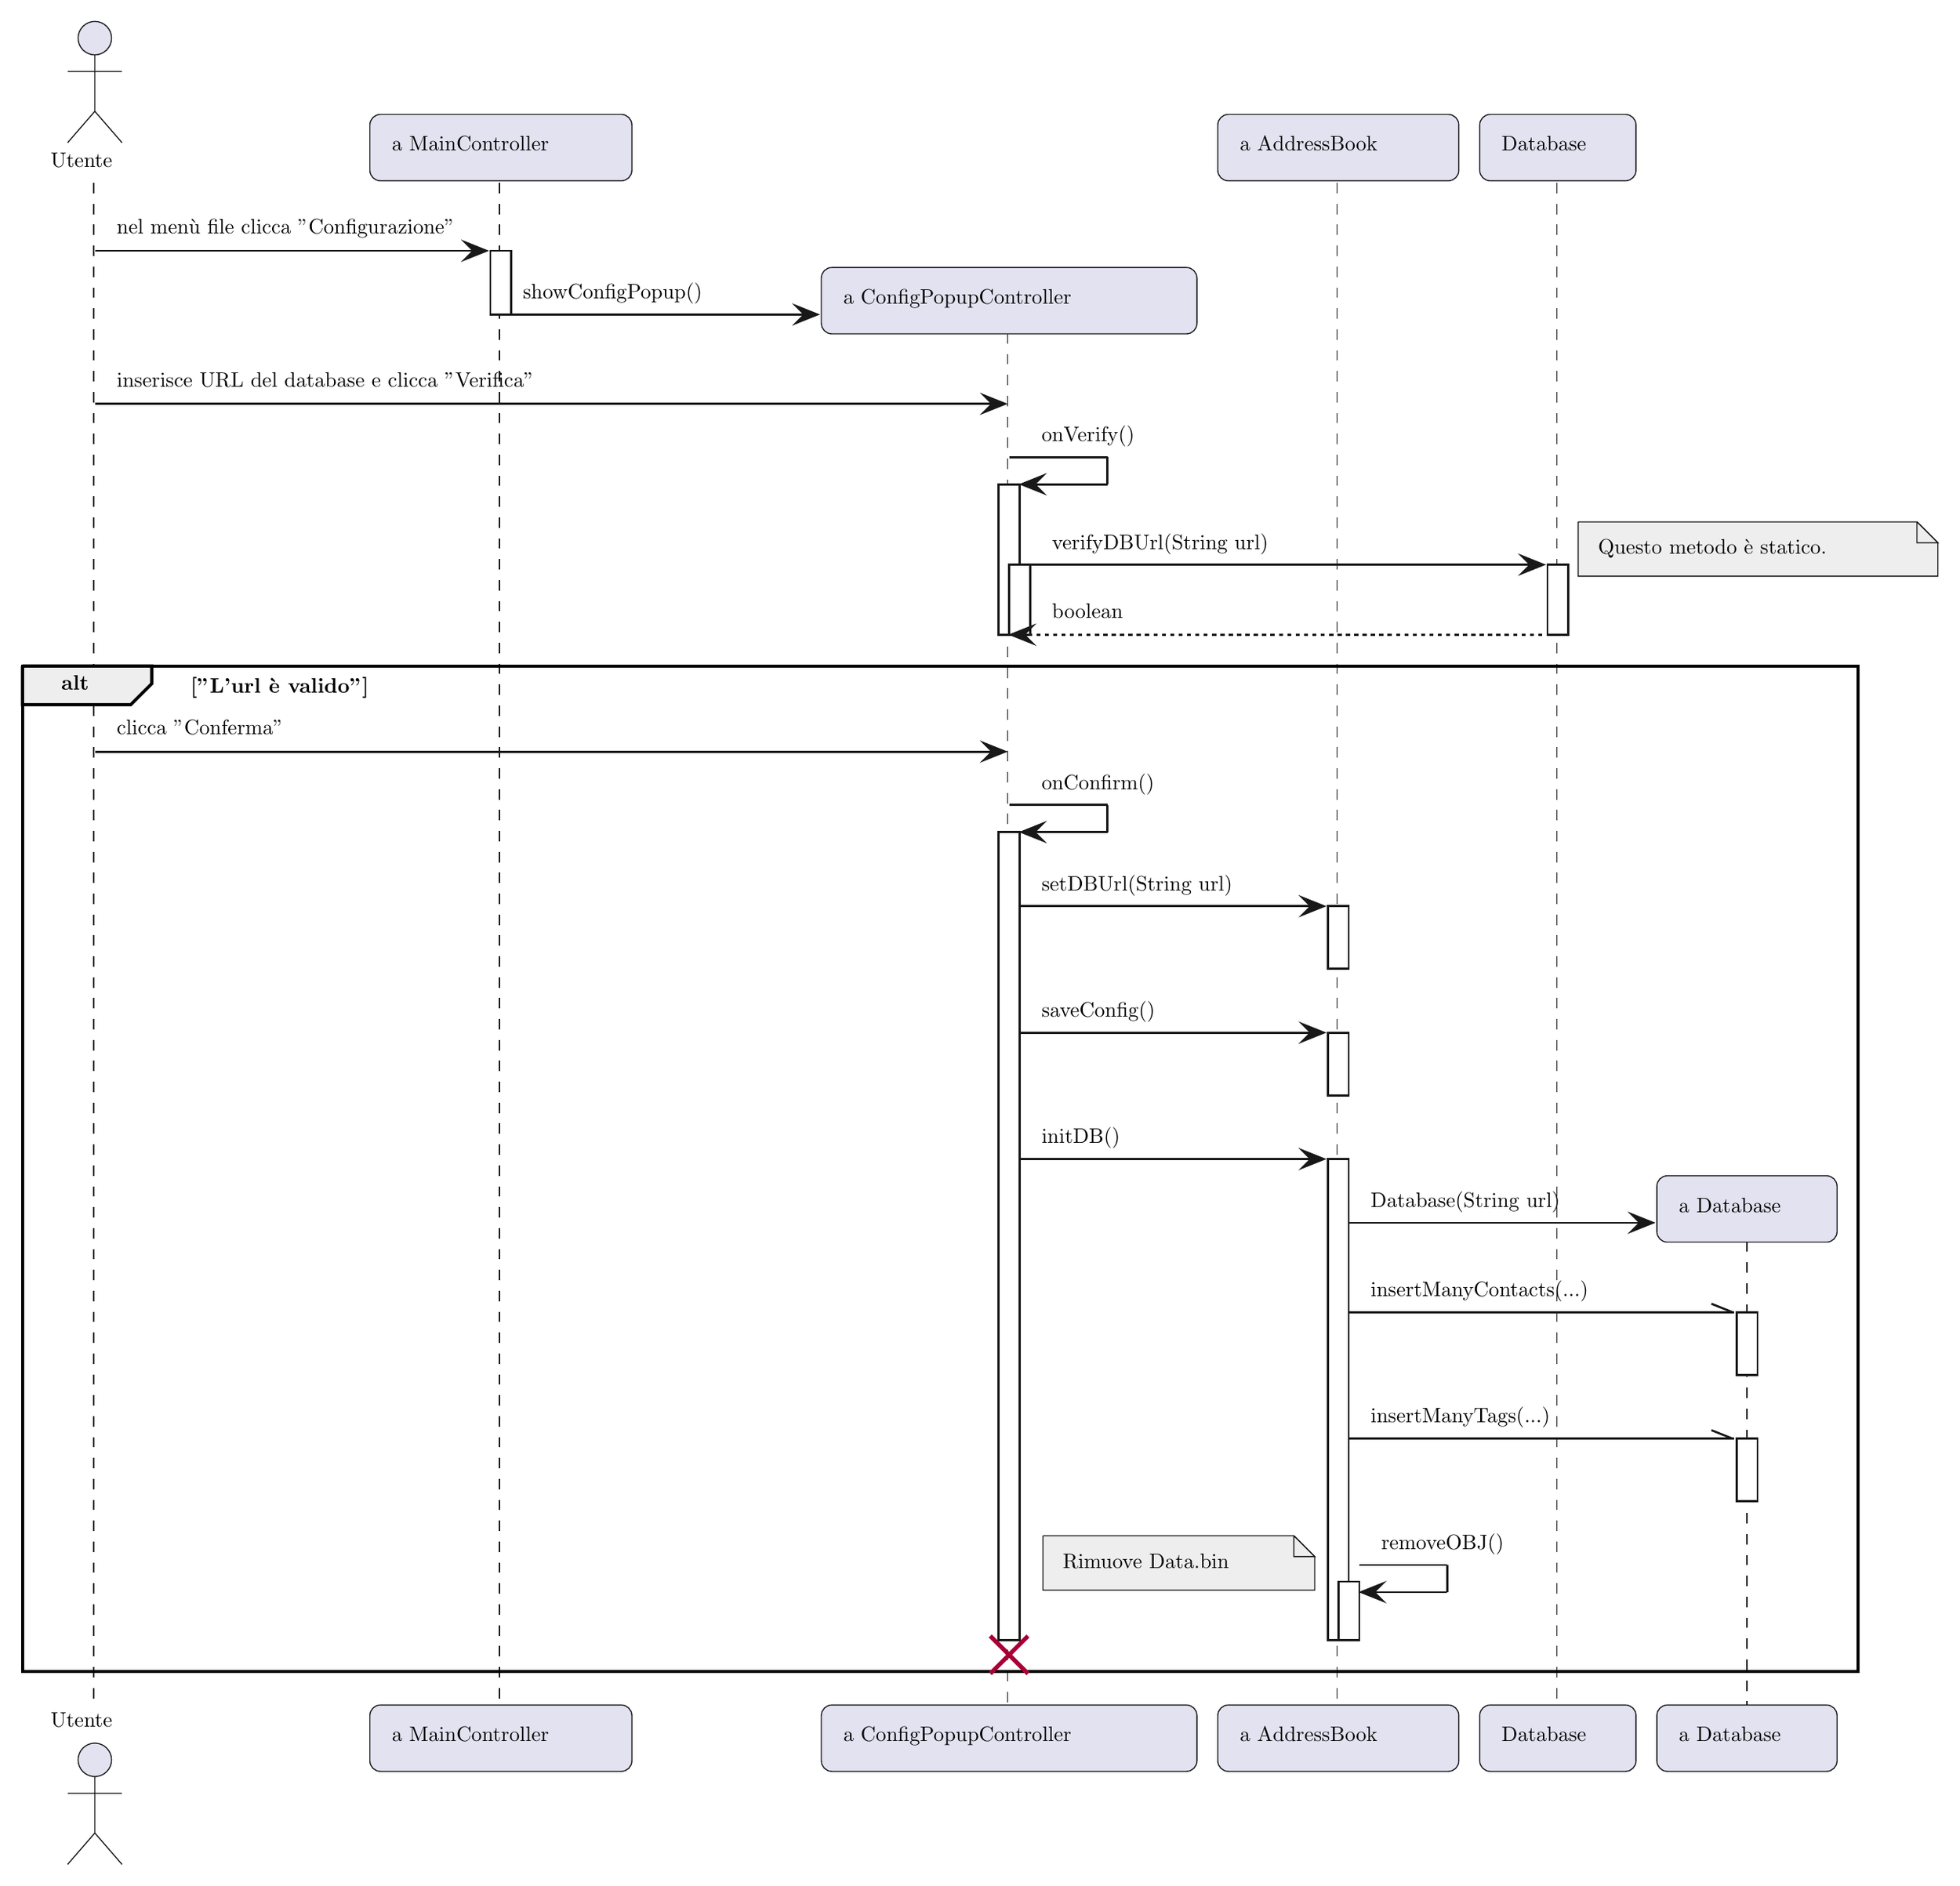
\begin{tikzpicture}[yscale=-1
,pstyle0/.style={color=plantucolor0001,fill=white,line width=1.0pt}
,pstyle1/.style={color=black,line width=1.5pt}
,pstyle2/.style={color=plantucolor0001,line width=0.5pt,dash pattern=on 5.0pt off 5.0pt}
,pstyle3/.style={color=plantucolor0001,fill=plantucolor0003,line width=0.5pt}
,pstyle4/.style={color=plantucolor0001,line width=0.5pt}
,pstyle5/.style={color=plantucolor0001,fill=plantucolor0001,line width=1.0pt}
,pstyle6/.style={color=plantucolor0001,line width=1.0pt}
,pstyle7/.style={color=plantucolor0001,fill=plantucolor0004,line width=0.5pt}
,pstyle10/.style={color=plantucolor0006,line width=2.0pt}
]
\draw[pstyle0] (233.7801pt,115.2246pt) rectangle (243.7801pt,145.7031pt);
\draw[pstyle0] (476.8468pt,226.9277pt) rectangle (486.8468pt,298.8848pt);
\draw[pstyle0] (481.8468pt,265.4063pt) rectangle (491.8468pt,298.8848pt);
\draw[pstyle0] (476.8468pt,393.3203pt) rectangle (486.8468pt,779.9375pt);
\draw[pstyle0] (634.2703pt,428.7988pt) rectangle (644.2703pt,458.7988pt);
\draw[pstyle0] (634.2703pt,489.2773pt) rectangle (644.2703pt,519.2773pt);
\draw[pstyle0] (634.2703pt,549.7559pt) rectangle (644.2703pt,779.9375pt);
\draw[pstyle0] (639.2703pt,751.9375pt) rectangle (649.2703pt,779.9375pt);
\draw[pstyle0] (739.2586pt,265.4063pt) rectangle (749.2586pt,298.8848pt);
\draw[pstyle0] (829.6987pt,622.9805pt) rectangle (839.6987pt,652.9805pt);
\draw[pstyle0] (829.6987pt,683.459pt) rectangle (839.6987pt,713.459pt);
\draw[pstyle1] (10pt,313.8848pt) rectangle (887.7741pt,794.9375pt);
\draw[pstyle2] (44pt,82.7461pt) -- (44pt,811.9375pt);
\draw[pstyle2] (238.1461pt,82.7461pt) -- (238.1461pt,811.9375pt);
\draw[pstyle2] (481.0468pt,154.5977pt) -- (481.0468pt,811.9375pt);
\draw[pstyle2] (638.6468pt,82.7461pt) -- (638.6468pt,811.9375pt);
\draw[pstyle2] (743.8939pt,82.7461pt) -- (743.8939pt,811.9375pt);
\draw[pstyle2] (834.6233pt,589.1289pt) -- (834.6233pt,811.9375pt);
\node at (20pt,65pt)[below right,color=black]{Utente};
\draw[pstyle3] (44.6pt,13.5pt) ellipse (8pt and 8pt);
\draw[pstyle4] (44.6pt,21.5pt) -- (44.6pt,48.5pt)(31.6pt,29.5pt) -- (57.6pt,29.5pt)(44.6pt,48.5pt) -- (31.6pt,63.5pt)(44.6pt,48.5pt) -- (57.6pt,63.5pt);
\node at (20pt,810.9375pt)[below right,color=black]{Utente};
\draw[pstyle3] (44.6pt,837.1836pt) ellipse (8pt and 8pt);
\draw[pstyle4] (44.6pt,845.1836pt) -- (44.6pt,872.1836pt)(31.6pt,853.1836pt) -- (57.6pt,853.1836pt)(44.6pt,872.1836pt) -- (31.6pt,887.1836pt)(44.6pt,872.1836pt) -- (57.6pt,887.1836pt);
\draw[pstyle3] (176.1461pt,55pt) arc (180:270:5pt) -- (181.1461pt,50pt) -- (296.4142pt,50pt) arc (270:360:5pt) -- (301.4142pt,55pt) -- (301.4142pt,76.7461pt) arc (0:90:5pt) -- (296.4142pt,81.7461pt) -- (181.1461pt,81.7461pt) arc (90:180:5pt) -- (176.1461pt,76.7461pt) -- cycle;
\node at (183.1461pt,57pt)[below right,color=black]{a MainController};
\draw[pstyle3] (176.1461pt,815.9375pt) arc (180:270:5pt) -- (181.1461pt,810.9375pt) -- (296.4142pt,810.9375pt) arc (270:360:5pt) -- (301.4142pt,815.9375pt) -- (301.4142pt,837.6836pt) arc (0:90:5pt) -- (296.4142pt,842.6836pt) -- (181.1461pt,842.6836pt) arc (90:180:5pt) -- (176.1461pt,837.6836pt) -- cycle;
\node at (183.1461pt,817.9375pt)[below right,color=black]{a MainController};
\draw[pstyle3] (392.0468pt,815.9375pt) arc (180:270:5pt) -- (397.0468pt,810.9375pt) -- (566.6468pt,810.9375pt) arc (270:360:5pt) -- (571.6468pt,815.9375pt) -- (571.6468pt,837.6836pt) arc (0:90:5pt) -- (566.6468pt,842.6836pt) -- (397.0468pt,842.6836pt) arc (90:180:5pt) -- (392.0468pt,837.6836pt) -- cycle;
\node at (399.0468pt,817.9375pt)[below right,color=black]{a ConfigPopupController};
\draw[pstyle3] (581.6468pt,55pt) arc (180:270:5pt) -- (586.6468pt,50pt) -- (691.8939pt,50pt) arc (270:360:5pt) -- (696.8939pt,55pt) -- (696.8939pt,76.7461pt) arc (0:90:5pt) -- (691.8939pt,81.7461pt) -- (586.6468pt,81.7461pt) arc (90:180:5pt) -- (581.6468pt,76.7461pt) -- cycle;
\node at (588.6468pt,57pt)[below right,color=black]{a AddressBook};
\draw[pstyle3] (581.6468pt,815.9375pt) arc (180:270:5pt) -- (586.6468pt,810.9375pt) -- (691.8939pt,810.9375pt) arc (270:360:5pt) -- (696.8939pt,815.9375pt) -- (696.8939pt,837.6836pt) arc (0:90:5pt) -- (691.8939pt,842.6836pt) -- (586.6468pt,842.6836pt) arc (90:180:5pt) -- (581.6468pt,837.6836pt) -- cycle;
\node at (588.6468pt,817.9375pt)[below right,color=black]{a AddressBook};
\draw[pstyle3] (706.8939pt,55pt) arc (180:270:5pt) -- (711.8939pt,50pt) -- (776.6233pt,50pt) arc (270:360:5pt) -- (781.6233pt,55pt) -- (781.6233pt,76.7461pt) arc (0:90:5pt) -- (776.6233pt,81.7461pt) -- (711.8939pt,81.7461pt) arc (90:180:5pt) -- (706.8939pt,76.7461pt) -- cycle;
\node at (713.8939pt,57pt)[below right,color=black]{Database};
\draw[pstyle3] (706.8939pt,815.9375pt) arc (180:270:5pt) -- (711.8939pt,810.9375pt) -- (776.6233pt,810.9375pt) arc (270:360:5pt) -- (781.6233pt,815.9375pt) -- (781.6233pt,837.6836pt) arc (0:90:5pt) -- (776.6233pt,842.6836pt) -- (711.8939pt,842.6836pt) arc (90:180:5pt) -- (706.8939pt,837.6836pt) -- cycle;
\node at (713.8939pt,817.9375pt)[below right,color=black]{Database};
\draw[pstyle3] (791.6233pt,815.9375pt) arc (180:270:5pt) -- (796.6233pt,810.9375pt) -- (872.7741pt,810.9375pt) arc (270:360:5pt) -- (877.7741pt,815.9375pt) -- (877.7741pt,837.6836pt) arc (0:90:5pt) -- (872.7741pt,842.6836pt) -- (796.6233pt,842.6836pt) arc (90:180:5pt) -- (791.6233pt,837.6836pt) -- cycle;
\node at (798.6233pt,817.9375pt)[below right,color=black]{a Database};
\draw[pstyle0] (233.7801pt,115.2246pt) rectangle (243.7801pt,145.7031pt);
\draw[pstyle0] (476.8468pt,226.9277pt) rectangle (486.8468pt,298.8848pt);
\draw[pstyle0] (481.8468pt,265.4063pt) rectangle (491.8468pt,298.8848pt);
\draw[pstyle0] (476.8468pt,393.3203pt) rectangle (486.8468pt,779.9375pt);
\draw[pstyle0] (634.2703pt,428.7988pt) rectangle (644.2703pt,458.7988pt);
\draw[pstyle0] (634.2703pt,489.2773pt) rectangle (644.2703pt,519.2773pt);
\draw[pstyle0] (634.2703pt,549.7559pt) rectangle (644.2703pt,779.9375pt);
\draw[pstyle0] (639.2703pt,751.9375pt) rectangle (649.2703pt,779.9375pt);
\draw[pstyle0] (739.2586pt,265.4063pt) rectangle (749.2586pt,298.8848pt);
\draw[pstyle0] (829.6987pt,622.9805pt) rectangle (839.6987pt,652.9805pt);
\draw[pstyle0] (829.6987pt,683.459pt) rectangle (839.6987pt,713.459pt);
\draw[pstyle5] (221.7801pt,111.2246pt) -- (231.7801pt,115.2246pt) -- (221.7801pt,119.2246pt) -- (225.7801pt,115.2246pt) -- cycle;
\draw[pstyle6] (44.6pt,115.2246pt) -- (227.7801pt,115.2246pt);
\node at (51.6pt,96.7461pt)[below right,color=black]{nel menù file clicca "Configurazione"};
\draw[pstyle5] (380.0468pt,141.7031pt) -- (390.0468pt,145.7031pt) -- (380.0468pt,149.7031pt) -- (384.0468pt,145.7031pt) -- cycle;
\draw[pstyle6] (238.7801pt,145.7031pt) -- (386.0468pt,145.7031pt);
\node at (245.7801pt,127.2246pt)[below right,color=black]{showConfigPopup()};
\draw[pstyle3] (392.0468pt,128.2246pt) arc (180:270:5pt) -- (397.0468pt,123.2246pt) -- (566.6468pt,123.2246pt) arc (270:360:5pt) -- (571.6468pt,128.2246pt) -- (571.6468pt,149.9707pt) arc (0:90:5pt) -- (566.6468pt,154.9707pt) -- (397.0468pt,154.9707pt) arc (90:180:5pt) -- (392.0468pt,149.9707pt) -- cycle;
\node at (399.0468pt,130.2246pt)[below right,color=black]{a ConfigPopupController};
\draw[pstyle5] (469.8468pt,184.4492pt) -- (479.8468pt,188.4492pt) -- (469.8468pt,192.4492pt) -- (473.8468pt,188.4492pt) -- cycle;
\draw[pstyle6] (44.6pt,188.4492pt) -- (475.8468pt,188.4492pt);
\node at (51.6pt,169.9707pt)[below right,color=black]{inserisce URL del database e clicca "Verifica"};
\draw[pstyle6] (481.8468pt,213.9277pt) -- (528.8468pt,213.9277pt);
\draw[pstyle6] (528.8468pt,213.9277pt) -- (528.8468pt,226.9277pt);
\draw[pstyle6] (487.8468pt,226.9277pt) -- (528.8468pt,226.9277pt);
\draw[pstyle5] (497.8468pt,222.9277pt) -- (487.8468pt,226.9277pt) -- (497.8468pt,230.9277pt) -- (493.8468pt,226.9277pt) -- cycle;
\node at (493.8468pt,195.4492pt)[below right,color=black]{onVerify()};
\draw[pstyle5] (727.2586pt,261.4063pt) -- (737.2586pt,265.4063pt) -- (727.2586pt,269.4063pt) -- (731.2586pt,265.4063pt) -- cycle;
\draw[pstyle6] (491.8468pt,265.4063pt) -- (733.2586pt,265.4063pt);
\node at (498.8468pt,246.9277pt)[below right,color=black]{verifyDBUrl(String url)};
\draw[pstyle7] (754pt,244.9277pt) -- (754pt,270.9277pt) -- (926pt,270.9277pt) -- (926pt,254.9277pt) -- (916pt,244.9277pt) -- (754pt,244.9277pt);
\draw[pstyle7] (916pt,244.9277pt) -- (916pt,254.9277pt) -- (926pt,254.9277pt) -- (916pt,244.9277pt);
\node at (760pt,249.9277pt)[below right,color=black]{Questo metodo è statico.};
\draw[pstyle5] (492.8468pt,294.8848pt) -- (482.8468pt,298.8848pt) -- (492.8468pt,302.8848pt) -- (488.8468pt,298.8848pt) -- cycle;
\draw[color=plantucolor0001,line width=1.0pt,dash pattern=on 2.0pt off 2.0pt] (486.8468pt,298.8848pt) -- (743.2586pt,298.8848pt);
\node at (498.8468pt,280.4063pt)[below right,color=black]{boolean};
\draw[color=black,fill=plantucolor0005,line width=1.5pt] (10pt,313.8848pt) -- (71.8pt,313.8848pt) -- (71.8pt,322.3633pt) -- (61.8pt,332.3633pt) -- (10pt,332.3633pt) -- (10pt,313.8848pt);
\draw[pstyle1] (10pt,313.8848pt) rectangle (887.7741pt,794.9375pt);
\node at (25pt,314.8848pt)[below right,color=black]{\textbf{alt}};
\node at (86.8pt,315.8848pt)[below right,color=black]{\textbf{["L'url è valido"]}};
\draw[pstyle5] (469.8468pt,350.8418pt) -- (479.8468pt,354.8418pt) -- (469.8468pt,358.8418pt) -- (473.8468pt,354.8418pt) -- cycle;
\draw[pstyle6] (44.6pt,354.8418pt) -- (475.8468pt,354.8418pt);
\node at (51.6pt,336.3633pt)[below right,color=black]{clicca "Conferma"};
\draw[pstyle6] (481.8468pt,380.3203pt) -- (528.8468pt,380.3203pt);
\draw[pstyle6] (528.8468pt,380.3203pt) -- (528.8468pt,393.3203pt);
\draw[pstyle6] (487.8468pt,393.3203pt) -- (528.8468pt,393.3203pt);
\draw[pstyle5] (497.8468pt,389.3203pt) -- (487.8468pt,393.3203pt) -- (497.8468pt,397.3203pt) -- (493.8468pt,393.3203pt) -- cycle;
\node at (493.8468pt,361.8418pt)[below right,color=black]{onConfirm()};
\draw[pstyle5] (622.2703pt,424.7988pt) -- (632.2703pt,428.7988pt) -- (622.2703pt,432.7988pt) -- (626.2703pt,428.7988pt) -- cycle;
\draw[pstyle6] (486.8468pt,428.7988pt) -- (628.2703pt,428.7988pt);
\node at (493.8468pt,410.3203pt)[below right,color=black]{setDBUrl(String url)};
\draw[pstyle5] (622.2703pt,485.2773pt) -- (632.2703pt,489.2773pt) -- (622.2703pt,493.2773pt) -- (626.2703pt,489.2773pt) -- cycle;
\draw[pstyle6] (486.8468pt,489.2773pt) -- (628.2703pt,489.2773pt);
\node at (493.8468pt,470.7988pt)[below right,color=black]{saveConfig()};
\draw[pstyle5] (622.2703pt,545.7559pt) -- (632.2703pt,549.7559pt) -- (622.2703pt,553.7559pt) -- (626.2703pt,549.7559pt) -- cycle;
\draw[pstyle6] (486.8468pt,549.7559pt) -- (628.2703pt,549.7559pt);
\node at (493.8468pt,531.2773pt)[below right,color=black]{initDB()};
\draw[pstyle5] (779.6233pt,576.2344pt) -- (789.6233pt,580.2344pt) -- (779.6233pt,584.2344pt) -- (783.6233pt,580.2344pt) -- cycle;
\draw[pstyle6] (644.2703pt,580.2344pt) -- (785.6233pt,580.2344pt);
\node at (651.2703pt,561.7559pt)[below right,color=black]{Database(String url)};
\draw[pstyle3] (791.6233pt,562.7559pt) arc (180:270:5pt) -- (796.6233pt,557.7559pt) -- (872.7741pt,557.7559pt) arc (270:360:5pt) -- (877.7741pt,562.7559pt) -- (877.7741pt,584.502pt) arc (0:90:5pt) -- (872.7741pt,589.502pt) -- (796.6233pt,589.502pt) arc (90:180:5pt) -- (791.6233pt,584.502pt) -- cycle;
\node at (798.6233pt,564.7559pt)[below right,color=black]{a Database};
\draw[pstyle6] (827.6987pt,622.9805pt) -- (817.6987pt,618.9805pt);
\draw[pstyle6] (644.2703pt,622.9805pt) -- (828.6987pt,622.9805pt);
\node at (651.2703pt,604.502pt)[below right,color=black]{insertManyContacts(...)};
\draw[pstyle6] (827.6987pt,683.459pt) -- (817.6987pt,679.459pt);
\draw[pstyle6] (644.2703pt,683.459pt) -- (828.6987pt,683.459pt);
\node at (651.2703pt,664.9805pt)[below right,color=black]{insertManyTags(...)};
\draw[pstyle6] (649.2703pt,743.9375pt) -- (691.2703pt,743.9375pt);
\draw[pstyle6] (691.2703pt,743.9375pt) -- (691.2703pt,756.9375pt);
\draw[pstyle6] (650.2703pt,756.9375pt) -- (691.2703pt,756.9375pt);
\draw[pstyle5] (660.2703pt,752.9375pt) -- (650.2703pt,756.9375pt) -- (660.2703pt,760.9375pt) -- (656.2703pt,756.9375pt) -- cycle;
\node at (656.2703pt,725.459pt)[below right,color=black]{removeOBJ()};
\draw[pstyle7] (498pt,729.959pt) -- (498pt,755.959pt) -- (628pt,755.959pt) -- (628pt,739.959pt) -- (618pt,729.959pt) -- (498pt,729.959pt);
\draw[pstyle7] (618pt,729.959pt) -- (618pt,739.959pt) -- (628pt,739.959pt) -- (618pt,729.959pt);
\node at (504pt,734.959pt)[below right,color=black]{Rimuove Data.bin};
\draw[pstyle10] (472.8468pt,777.9375pt) -- (490.8468pt,795.9375pt);
\draw[pstyle10] (472.8468pt,795.9375pt) -- (490.8468pt,777.9375pt);
\end{tikzpicture}
}
\end{adjustbox}

\begin{figure}[h]
	\caption{Diagramma sequenza Aggiunta DB}
	\label{fig:Diagramma sequenza Aggiunta DB}
\end{figure}

\newpage
\subsubsection{Inizializzazione rubrica}
Il seguente diagramma di sequenza illustra il flusso di operazioni eseguito quando l'utente apre l'applicazione, durante la fase di inizializzazione, permettendogli di recuperare tutti i contatti della sessione precedente, attraverso il DB o il file \texttt{Data.bin}:
% generated by Plantuml 1.2024.3       
\definecolor{plantucolor0000}{RGB}{255,255,255}
\definecolor{plantucolor0001}{RGB}{24,24,24}
\definecolor{plantucolor0002}{RGB}{0,0,0}
\definecolor{plantucolor0003}{RGB}{226,226,240}
\definecolor{plantucolor0004}{RGB}{238,238,238}

\begin{adjustbox}{width=.82\paperwidth, center}
	\resizebox{\textwidth}{!}{
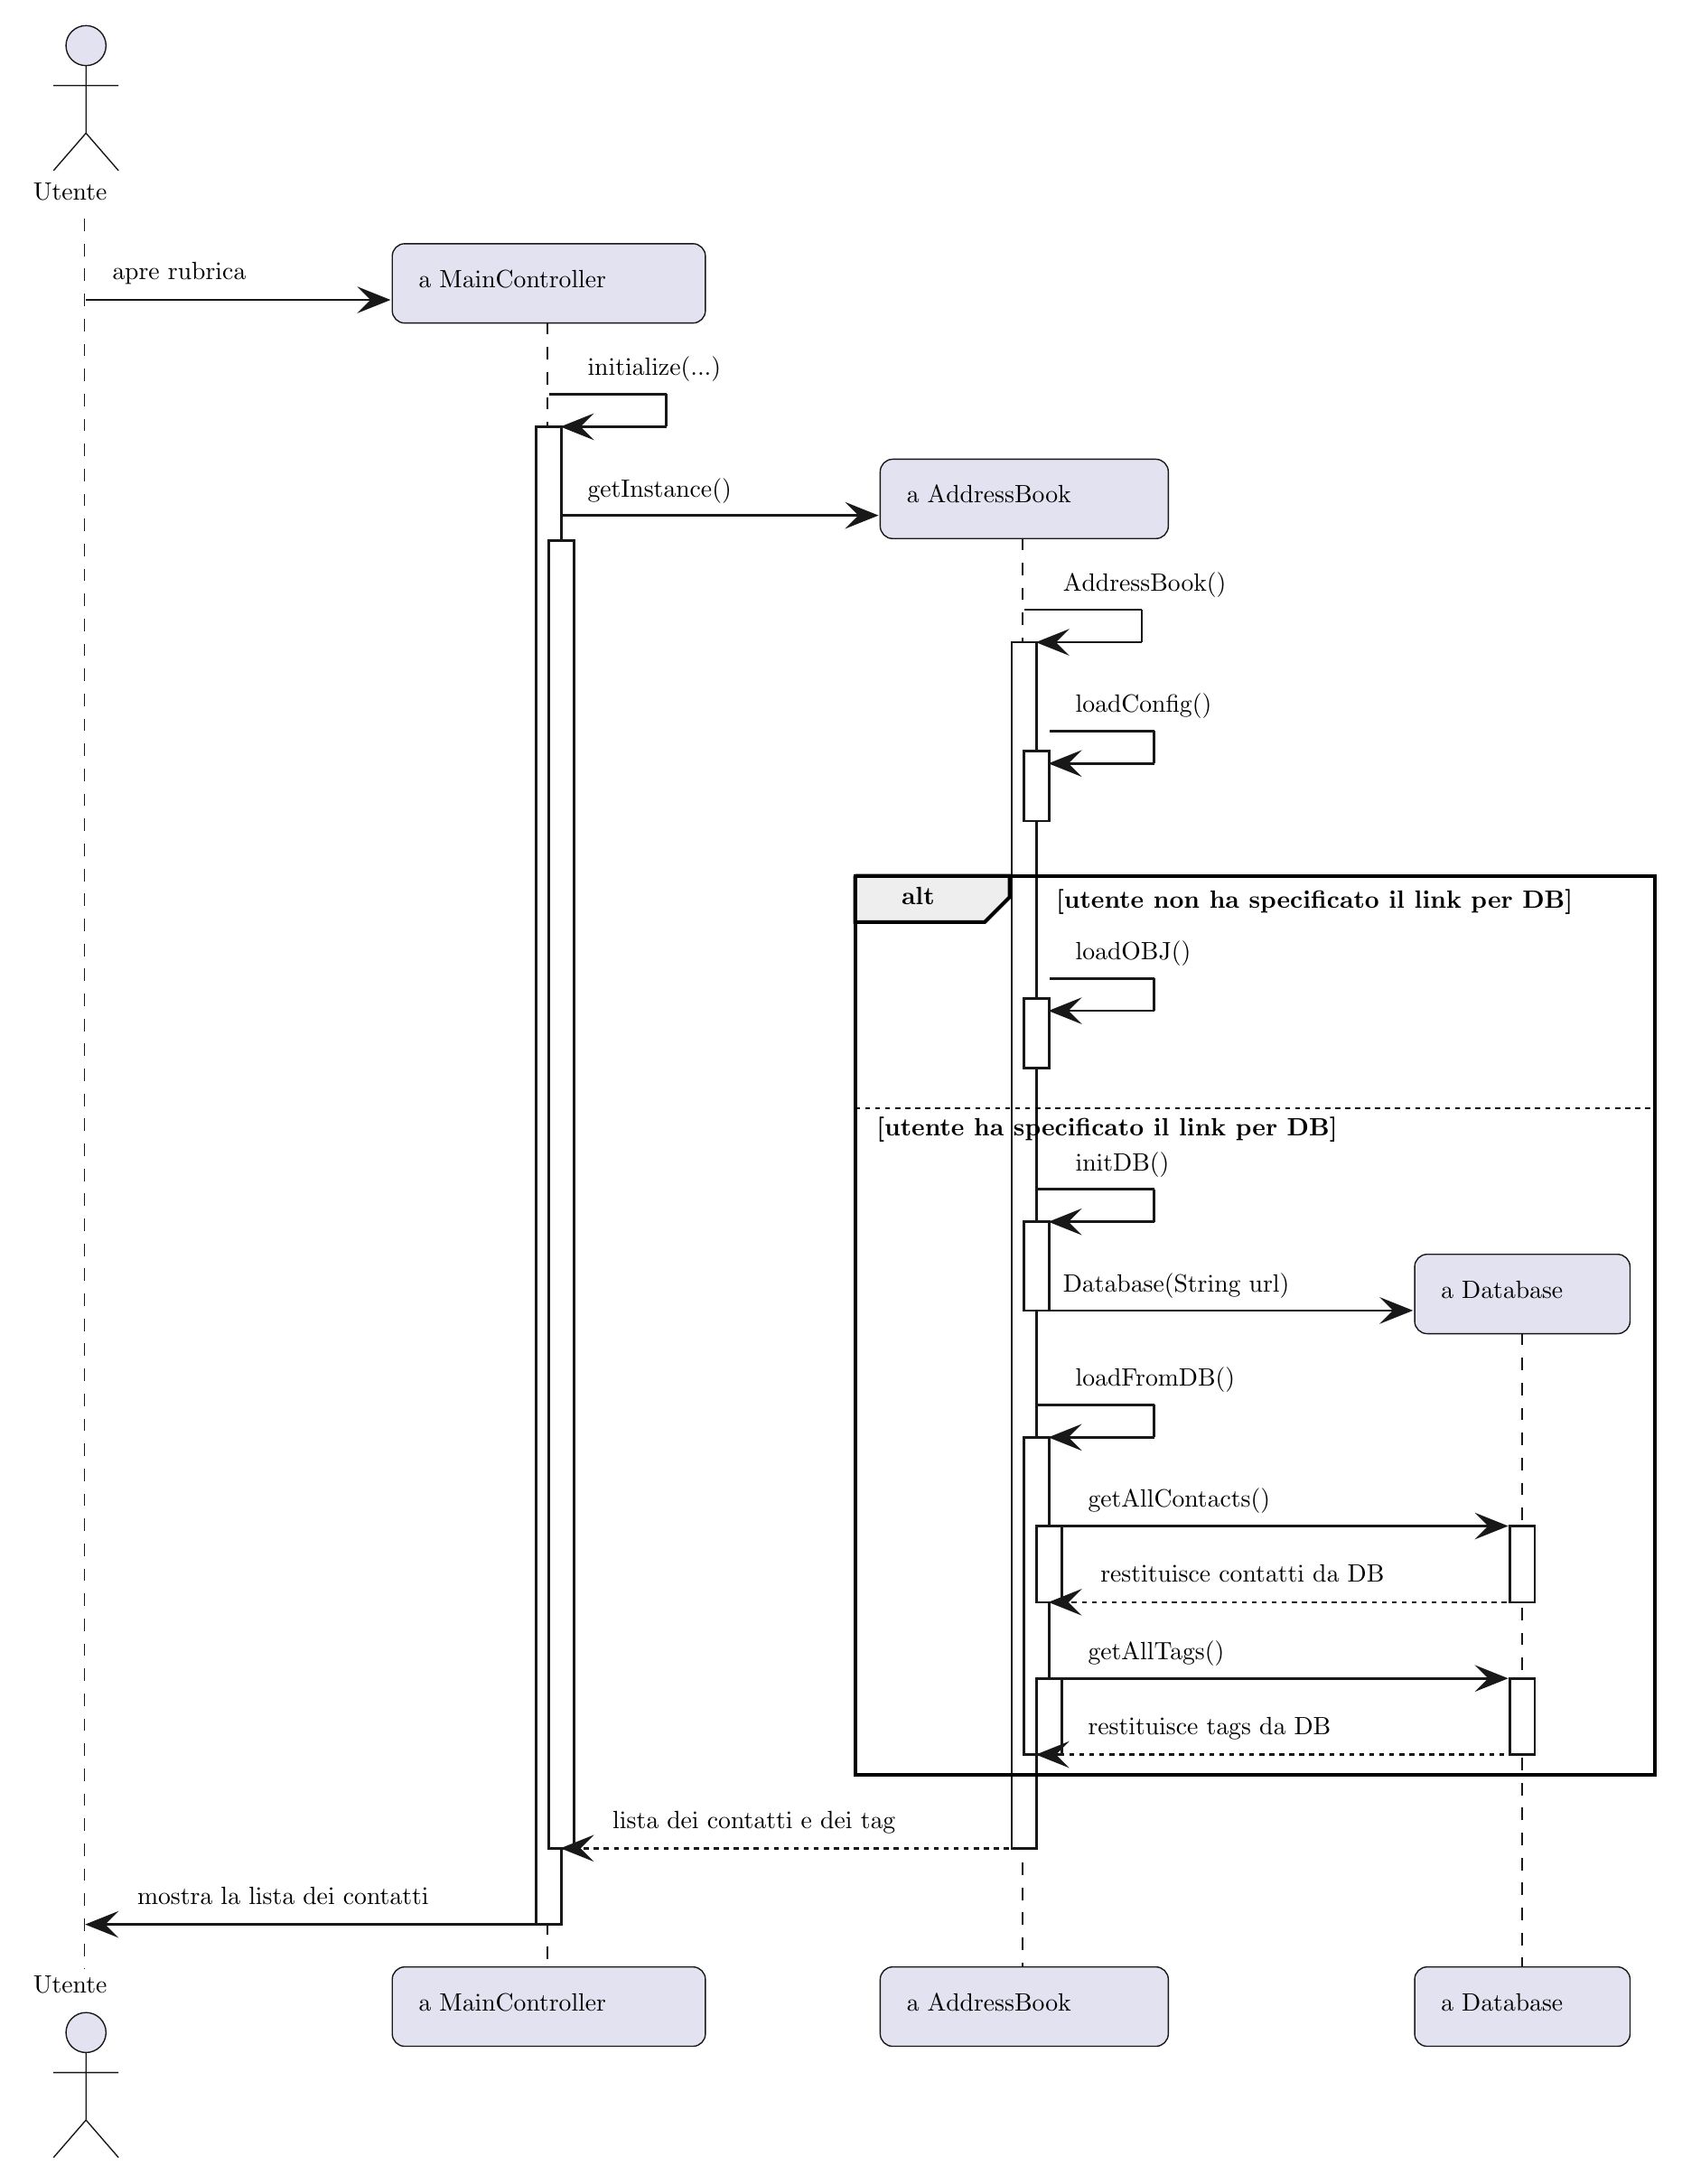
\begin{tikzpicture}[yscale=-1
,pstyle0/.style={color=plantucolor0001,fill=white,line width=1.0pt}
,pstyle1/.style={color=black,line width=1.5pt}
,pstyle2/.style={color=plantucolor0001,line width=0.5pt,dash pattern=on 5.0pt off 5.0pt}
,pstyle3/.style={color=plantucolor0001,fill=plantucolor0003,line width=0.5pt}
,pstyle4/.style={color=plantucolor0001,line width=0.5pt}
,pstyle5/.style={color=plantucolor0001,fill=plantucolor0001,line width=1.0pt}
,pstyle6/.style={color=plantucolor0001,line width=1.0pt}
,pstyle9/.style={color=plantucolor0001,line width=1.0pt,dash pattern=on 2.0pt off 2.0pt}
]
\draw[pstyle0] (209.7412pt,165.9707pt) rectangle (219.7412pt,765.1484pt);
\draw[pstyle0] (214.7412pt,211.4492pt) rectangle (224.7412pt,734.6699pt);
\draw[pstyle0] (399.9201pt,252.1953pt) rectangle (409.9201pt,734.6699pt);
\draw[pstyle0] (404.9201pt,295.6738pt) rectangle (414.9201pt,323.6738pt);
\draw[pstyle0] (404.9201pt,394.6309pt) rectangle (414.9201pt,422.6309pt);
\draw[pstyle0] (404.9201pt,484.0527pt) rectangle (414.9201pt,519.5313pt);
\draw[pstyle0] (404.9201pt,570.2773pt) rectangle (414.9201pt,697.1914pt);
\draw[pstyle0] (409.9201pt,605.7559pt) rectangle (419.9201pt,636.2344pt);
\draw[pstyle0] (409.9201pt,666.7129pt) rectangle (419.9201pt,697.1914pt);
\draw[pstyle0] (599.1646pt,605.7559pt) rectangle (609.1646pt,636.2344pt);
\draw[pstyle0] (599.1646pt,666.7129pt) rectangle (609.1646pt,697.1914pt);
\draw[pstyle1] (337.2966pt,345.6738pt) rectangle (657.24pt,705.1914pt);
\draw[pstyle2] (29pt,82.7461pt) -- (29pt,783.1484pt);
\draw[pstyle2] (214.1071pt,124.1191pt) -- (214.1071pt,783.1484pt);
\draw[pstyle2] (404.2966pt,210.3438pt) -- (404.2966pt,783.1484pt);
\draw[pstyle2] (604.0892pt,528.4258pt) -- (604.0892pt,783.1484pt);
\node at (5pt,65pt)[below right,color=black]{Utente};
\draw[pstyle3] (29.6pt,13.5pt) ellipse (8pt and 8pt);
\draw[pstyle4] (29.6pt,21.5pt) -- (29.6pt,48.5pt)(16.6pt,29.5pt) -- (42.6pt,29.5pt)(29.6pt,48.5pt) -- (16.6pt,63.5pt)(29.6pt,48.5pt) -- (42.6pt,63.5pt);
\node at (5pt,782.1484pt)[below right,color=black]{Utente};
\draw[pstyle3] (29.6pt,808.3945pt) ellipse (8pt and 8pt);
\draw[pstyle4] (29.6pt,816.3945pt) -- (29.6pt,843.3945pt)(16.6pt,824.3945pt) -- (42.6pt,824.3945pt)(29.6pt,843.3945pt) -- (16.6pt,858.3945pt)(29.6pt,843.3945pt) -- (42.6pt,858.3945pt);
\draw[pstyle3] (152.1071pt,787.1484pt) arc (180:270:5pt) -- (157.1071pt,782.1484pt) -- (272.3752pt,782.1484pt) arc (270:360:5pt) -- (277.3752pt,787.1484pt) -- (277.3752pt,808.8945pt) arc (0:90:5pt) -- (272.3752pt,813.8945pt) -- (157.1071pt,813.8945pt) arc (90:180:5pt) -- (152.1071pt,808.8945pt) -- cycle;
\node at (159.1071pt,789.1484pt)[below right,color=black]{a MainController};
\draw[pstyle3] (347.2966pt,787.1484pt) arc (180:270:5pt) -- (352.2966pt,782.1484pt) -- (457.5437pt,782.1484pt) arc (270:360:5pt) -- (462.5437pt,787.1484pt) -- (462.5437pt,808.8945pt) arc (0:90:5pt) -- (457.5437pt,813.8945pt) -- (352.2966pt,813.8945pt) arc (90:180:5pt) -- (347.2966pt,808.8945pt) -- cycle;
\node at (354.2966pt,789.1484pt)[below right,color=black]{a AddressBook};
\draw[pstyle3] (561.0892pt,787.1484pt) arc (180:270:5pt) -- (566.0892pt,782.1484pt) -- (642.24pt,782.1484pt) arc (270:360:5pt) -- (647.24pt,787.1484pt) -- (647.24pt,808.8945pt) arc (0:90:5pt) -- (642.24pt,813.8945pt) -- (566.0892pt,813.8945pt) arc (90:180:5pt) -- (561.0892pt,808.8945pt) -- cycle;
\node at (568.0892pt,789.1484pt)[below right,color=black]{a Database};
\draw[pstyle0] (209.7412pt,165.9707pt) rectangle (219.7412pt,765.1484pt);
\draw[pstyle0] (214.7412pt,211.4492pt) rectangle (224.7412pt,734.6699pt);
\draw[pstyle0] (399.9201pt,252.1953pt) rectangle (409.9201pt,734.6699pt);
\draw[pstyle0] (404.9201pt,295.6738pt) rectangle (414.9201pt,323.6738pt);
\draw[pstyle0] (404.9201pt,394.6309pt) rectangle (414.9201pt,422.6309pt);
\draw[pstyle0] (404.9201pt,484.0527pt) rectangle (414.9201pt,519.5313pt);
\draw[pstyle0] (404.9201pt,570.2773pt) rectangle (414.9201pt,697.1914pt);
\draw[pstyle0] (409.9201pt,605.7559pt) rectangle (419.9201pt,636.2344pt);
\draw[pstyle0] (409.9201pt,666.7129pt) rectangle (419.9201pt,697.1914pt);
\draw[pstyle0] (599.1646pt,605.7559pt) rectangle (609.1646pt,636.2344pt);
\draw[pstyle0] (599.1646pt,666.7129pt) rectangle (609.1646pt,697.1914pt);
\draw[pstyle5] (140.1071pt,111.2246pt) -- (150.1071pt,115.2246pt) -- (140.1071pt,119.2246pt) -- (144.1071pt,115.2246pt) -- cycle;
\draw[pstyle6] (29.6pt,115.2246pt) -- (146.1071pt,115.2246pt);
\node at (36.6pt,96.7461pt)[below right,color=black]{apre rubrica};
\draw[pstyle3] (152.1071pt,97.7461pt) arc (180:270:5pt) -- (157.1071pt,92.7461pt) -- (272.3752pt,92.7461pt) arc (270:360:5pt) -- (277.3752pt,97.7461pt) -- (277.3752pt,119.4922pt) arc (0:90:5pt) -- (272.3752pt,124.4922pt) -- (157.1071pt,124.4922pt) arc (90:180:5pt) -- (152.1071pt,119.4922pt) -- cycle;
\node at (159.1071pt,99.7461pt)[below right,color=black]{a MainController};
\draw[pstyle6] (214.7412pt,152.9707pt) -- (261.7412pt,152.9707pt);
\draw[pstyle6] (261.7412pt,152.9707pt) -- (261.7412pt,165.9707pt);
\draw[pstyle6] (220.7412pt,165.9707pt) -- (261.7412pt,165.9707pt);
\draw[pstyle5] (230.7412pt,161.9707pt) -- (220.7412pt,165.9707pt) -- (230.7412pt,169.9707pt) -- (226.7412pt,165.9707pt) -- cycle;
\node at (226.7412pt,134.4922pt)[below right,color=black]{initialize(...)};
\draw[pstyle5] (335.2966pt,197.4492pt) -- (345.2966pt,201.4492pt) -- (335.2966pt,205.4492pt) -- (339.2966pt,201.4492pt) -- cycle;
\draw[pstyle6] (219.7412pt,201.4492pt) -- (341.2966pt,201.4492pt);
\node at (226.7412pt,182.9707pt)[below right,color=black]{getInstance()};
\draw[pstyle3] (347.2966pt,183.9707pt) arc (180:270:5pt) -- (352.2966pt,178.9707pt) -- (457.5437pt,178.9707pt) arc (270:360:5pt) -- (462.5437pt,183.9707pt) -- (462.5437pt,205.7168pt) arc (0:90:5pt) -- (457.5437pt,210.7168pt) -- (352.2966pt,210.7168pt) arc (90:180:5pt) -- (347.2966pt,205.7168pt) -- cycle;
\node at (354.2966pt,185.9707pt)[below right,color=black]{a AddressBook};
\draw[pstyle6] (404.9201pt,239.1953pt) -- (451.9201pt,239.1953pt);
\draw[pstyle6] (451.9201pt,239.1953pt) -- (451.9201pt,252.1953pt);
\draw[pstyle6] (410.9201pt,252.1953pt) -- (451.9201pt,252.1953pt);
\draw[pstyle5] (420.9201pt,248.1953pt) -- (410.9201pt,252.1953pt) -- (420.9201pt,256.1953pt) -- (416.9201pt,252.1953pt) -- cycle;
\node at (416.9201pt,220.7168pt)[below right,color=black]{AddressBook()};
\draw[pstyle6] (414.9201pt,287.6738pt) -- (456.9201pt,287.6738pt);
\draw[pstyle6] (456.9201pt,287.6738pt) -- (456.9201pt,300.6738pt);
\draw[pstyle6] (415.9201pt,300.6738pt) -- (456.9201pt,300.6738pt);
\draw[pstyle5] (425.9201pt,296.6738pt) -- (415.9201pt,300.6738pt) -- (425.9201pt,304.6738pt) -- (421.9201pt,300.6738pt) -- cycle;
\node at (421.9201pt,269.1953pt)[below right,color=black]{loadConfig()};
\draw[color=black,fill=plantucolor0004,line width=1.5pt] (337.2966pt,345.6738pt) -- (399.0966pt,345.6738pt) -- (399.0966pt,354.1523pt) -- (389.0966pt,364.1523pt) -- (337.2966pt,364.1523pt) -- (337.2966pt,345.6738pt);
\draw[pstyle1] (337.2966pt,345.6738pt) rectangle (657.24pt,705.1914pt);
\node at (352.2966pt,346.6738pt)[below right,color=black]{\textbf{alt}};
\node at (414.0966pt,347.6738pt)[below right,color=black]{\textbf{[utente non ha specificato il link per DB]}};
\draw[pstyle6] (414.9201pt,386.6309pt) -- (456.9201pt,386.6309pt);
\draw[pstyle6] (456.9201pt,386.6309pt) -- (456.9201pt,399.6309pt);
\draw[pstyle6] (415.9201pt,399.6309pt) -- (456.9201pt,399.6309pt);
\draw[pstyle5] (425.9201pt,395.6309pt) -- (415.9201pt,399.6309pt) -- (425.9201pt,403.6309pt) -- (421.9201pt,399.6309pt) -- cycle;
\node at (421.9201pt,368.1523pt)[below right,color=black]{loadOBJ()};
\draw[color=black,line width=1.0pt,dash pattern=on 2.0pt off 2.0pt] (337.2966pt,438.6309pt) -- (657.24pt,438.6309pt);
\node at (342.2966pt,438.6309pt)[below right,color=black]{\textbf{[utente ha specificato il link per DB]}};
\draw[pstyle6] (409.9201pt,471.0527pt) -- (456.9201pt,471.0527pt);
\draw[pstyle6] (456.9201pt,471.0527pt) -- (456.9201pt,484.0527pt);
\draw[pstyle6] (415.9201pt,484.0527pt) -- (456.9201pt,484.0527pt);
\draw[pstyle5] (425.9201pt,480.0527pt) -- (415.9201pt,484.0527pt) -- (425.9201pt,488.0527pt) -- (421.9201pt,484.0527pt) -- cycle;
\node at (421.9201pt,452.5742pt)[below right,color=black]{initDB()};
\draw[pstyle5] (549.0892pt,515.5313pt) -- (559.0892pt,519.5313pt) -- (549.0892pt,523.5313pt) -- (553.0892pt,519.5313pt) -- cycle;
\draw[pstyle6] (409.9201pt,519.5313pt) -- (555.0892pt,519.5313pt);
\node at (416.9201pt,501.0527pt)[below right,color=black]{Database(String url)};
\draw[pstyle3] (561.0892pt,502.0527pt) arc (180:270:5pt) -- (566.0892pt,497.0527pt) -- (642.24pt,497.0527pt) arc (270:360:5pt) -- (647.24pt,502.0527pt) -- (647.24pt,523.7988pt) arc (0:90:5pt) -- (642.24pt,528.7988pt) -- (566.0892pt,528.7988pt) arc (90:180:5pt) -- (561.0892pt,523.7988pt) -- cycle;
\node at (568.0892pt,504.0527pt)[below right,color=black]{a Database};
\draw[pstyle6] (409.9201pt,557.2773pt) -- (456.9201pt,557.2773pt);
\draw[pstyle6] (456.9201pt,557.2773pt) -- (456.9201pt,570.2773pt);
\draw[pstyle6] (415.9201pt,570.2773pt) -- (456.9201pt,570.2773pt);
\draw[pstyle5] (425.9201pt,566.2773pt) -- (415.9201pt,570.2773pt) -- (425.9201pt,574.2773pt) -- (421.9201pt,570.2773pt) -- cycle;
\node at (421.9201pt,538.7988pt)[below right,color=black]{loadFromDB()};
\draw[pstyle5] (587.1646pt,601.7559pt) -- (597.1646pt,605.7559pt) -- (587.1646pt,609.7559pt) -- (591.1646pt,605.7559pt) -- cycle;
\draw[pstyle6] (419.9201pt,605.7559pt) -- (593.1646pt,605.7559pt);
\node at (426.9201pt,587.2773pt)[below right,color=black]{getAllContacts()};
\draw[pstyle5] (425.9201pt,632.2344pt) -- (415.9201pt,636.2344pt) -- (425.9201pt,640.2344pt) -- (421.9201pt,636.2344pt) -- cycle;
\draw[pstyle9] (419.9201pt,636.2344pt) -- (603.1646pt,636.2344pt);
\node at (431.9201pt,617.7559pt)[below right,color=black]{restituisce contatti da DB};
\draw[pstyle5] (587.1646pt,662.7129pt) -- (597.1646pt,666.7129pt) -- (587.1646pt,670.7129pt) -- (591.1646pt,666.7129pt) -- cycle;
\draw[pstyle6] (419.9201pt,666.7129pt) -- (593.1646pt,666.7129pt);
\node at (426.9201pt,648.2344pt)[below right,color=black]{getAllTags()};
\draw[pstyle5] (420.9201pt,693.1914pt) -- (410.9201pt,697.1914pt) -- (420.9201pt,701.1914pt) -- (416.9201pt,697.1914pt) -- cycle;
\draw[pstyle9] (414.9201pt,697.1914pt) -- (603.1646pt,697.1914pt);
\node at (426.9201pt,678.7129pt)[below right,color=black]{restituisce tags da DB};
\draw[pstyle5] (230.7412pt,730.6699pt) -- (220.7412pt,734.6699pt) -- (230.7412pt,738.6699pt) -- (226.7412pt,734.6699pt) -- cycle;
\draw[pstyle9] (224.7412pt,734.6699pt) -- (403.9201pt,734.6699pt);
\node at (236.7412pt,716.1914pt)[below right,color=black]{lista dei contatti e dei tag};
\draw[pstyle5] (40.6pt,761.1484pt) -- (30.6pt,765.1484pt) -- (40.6pt,769.1484pt) -- (36.6pt,765.1484pt) -- cycle;
\draw[pstyle6] (34.6pt,765.1484pt) -- (213.7412pt,765.1484pt);
\node at (46.6pt,746.6699pt)[below right,color=black]{mostra la lista dei contatti};
\end{tikzpicture}
}
\end{adjustbox}

\begin{figure}[h]
	\caption{Diagramma sequenza Inizializzazione rubrica}
	\label{fig:Diagramma sequenza Inizializzazione rubrica}
\end{figure}


\newpage
\subsection{Principi di buona progettazione}
Si garantisce l'aderenza ai principi di buona progettazione del software, migliorando modularità, manutenibilità e chiarezza del sistema.
\subsubsection{Livelli di coesione}
\begin{figure}[h]
	\centering
	\includegraphics[width=.9\linewidth]{images/Coesione classi.jpg}
	\caption{Livelli di coesione classi}
	\label{fig:livelli di coesione classi}
\end{figure}
\newpage
\subsubsection{Livelli di accoppiamento}
\begin{figure}[h]
	\centering
	\includegraphics[width=.9\linewidth]{images/Accoppiamento_classi.jpg}
	\caption{Livelli di accoppiamento classi}
	\label{fig:livelli di accoppiamento classi}
\end{figure}

\subsubsection{Relazioni tra le Classi}
Nel progetto si è prediletta l’associazione rispetto alla specializzazione (ereditarietà). \\
In particolare:
\begin{itemize}[noitemsep, topsep=5pt]
	\item Esiste una relazione di aggregazione 1 a molti tra \textit{AddressBook} e \textit{Contact}, tra \textit{AddressBook} e \textit{Tag}.
	\item È presente una relazione di composizione 1 a 0..1 tra \textit{AddressBook} e \textit{Database}, poiché la rubrica può prevedere il salvataggio su database o in locale.
\end{itemize}

\subsubsection{Riduzione dell’Accoppiamento}
Per seguire il principio di riduzione dell’accoppiamento tra classi, sono state create le interfacce \textit{TagManager} e \textit{ContactManager}. \\
Questo consente alle classi \textit{Export}, \textit{Import} e \textit{ManageTagsPopupController} di accedere solo ai metodi strettamente necessari, favorendo anche il principio di segregazione delle interfacce.\\
Tuttavia:
\begin{itemize}[noitemsep, topsep=5pt]
	\item \textit{MainController} ha un riferimento diretto a \textit{AddressBook}, poiché dipende da esso per la maggior parte dei metodi, esclusi quelli relativi ai tag.
	\item \textit{ConfigPopupController} ha anch’esso un riferimento diretto a \textit{AddressBook}, ma con un accoppiamento per timbro, dato che utilizza solo alcuni metodi.
\end{itemize}
\subsubsection{Relazione con l’Interfaccia Initializable}
Tutti i controller implementano l’interfaccia \textit{Initializable}, ma nei diagrammi di classe tale relazione viene omessa per ridurre il livello di dettaglio e garantire una maggiore visibilità.

\subsubsection{Livelli di dettaglio}
Sono forniti due diagrammi di classi con livelli di dettaglio differenti:
\begin{itemize}[noitemsep, topsep=5pt]
	\item Diagramma con relazioni evidenziate: Mostra solo i metodi e attributi più rilevanti, evidenziando meglio le relazioni.
	\item Diagramma completo: Descrive in dettaglio tutti gli attributi e metodi delle classi, evidenziandone più concretamente il ruolo nella realizzazione del sistema.
\end{itemize}

\subsubsection{Diagrammi di Sequenza}
Sono forniti diagrammi di sequenza per descrivere i flussi di eventi relativi all’interazione tra l’utente e la rubrica, tra cui:
\begin{itemize}[noitemsep, topsep=5pt]
	\item Alcuni casi d’uso specifici (C1, C2, C3, C5, C6, C8).
	\item L’operazione di aggiunta del database tramite link inserito dall’utente.
	\item Lo scenario di apertura e inizializzazione della rubrica, che può avvenire attraverso il database o il file locale \texttt{Data.bin} in assenza del database.
\end{itemize}